%% 
%% Copyright 2019-2020 Elsevier Ltd
%% 
%% This file is part of the 'CAS Bundle'.
%% --------------------------------------
%% 
%% It may be distributed under the conditions of the LaTeX Project Public
%% License, either version 1.2 of this license or (at your option) any
%% later version.  The latest version of this license is in
%%    http://www.latex-project.org/lppl.txt
%% and version 1.2 or later is part of all distributions of LaTeX
%% version 1999/12/01 or later.
%% 
%% The list of all files belonging to the 'CAS Bundle' is
%% given in the file `manifest.txt'.
%% 
%% Template article for cas-sc documentclass for 
%% double column output.

%\documentclass[a4paper,fleqn,longmktitle]{cas-sc}
\documentclass[a4paper,fleqn]{cas-sc}
\usepackage[utf8]{inputenc}
\usepackage{newunicodechar}
\newunicodechar{₂}{$_2$}
\newunicodechar{₅}{$_5$}
\usepackage{placeins}
 \usepackage[numbers]{natbib}
%\usepackage[authoryear]{natbib}
%\usepackage[authoryear,longnamesfirst]{natbib}
\usepackage{rotating}%
\usepackage{multirow}%
\usepackage{booktabs}%
\usepackage{graphicx}%
\usepackage{tikz}
\usepackage{graphicx}
\usepackage{amsmath}
\usepackage{xcolor}

\usetikzlibrary{
    arrows.meta,
    positioning,
    calc,
    fit,
    backgrounds,
    shapes.geometric
}

% ============================================================
% Colours
% ============================================================
\definecolor{titleblue}{RGB}{8,58,112}
\definecolor{lightblue}{RGB}{240,247,255}
\definecolor{lightgreen}{RGB}{244,252,239}
\definecolor{lightorange}{RGB}{255,249,232}
\definecolor{lightgray}{RGB}{249,249,249}
\definecolor{lightpurple}{RGB}{249,242,255}


% Overleaf: put PNG/PDF figures in ./figs/ (matches Elsevier convention). Repo also searches figures/ and reports/.
\graphicspath{{figs/}{figures/}{./}{reports/figures/}}
\usepackage{subcaption}
\usepackage{float}%
\usepackage{xcolor}%
\newcommand{\rev}[1]{\textcolor{blue}{#1}}%
\newcommand{\orig}[1]{{\color{blue}#1}}% original wording retained
\newcommand{\prop}[1]{{\color{red}#1}}% proposed replacement

%%%Author definitions
\def\tsc#1{\csdef{#1}{\textsc{\lowercase{#1}}\xspace}}
\tsc{WGM}
\tsc{QE}
\tsc{EP}
\tsc{PMS}
\tsc{BEC}
\tsc{DE}
%%%

% Uncomment and use as if needed
%\newtheorem{theorem}{Theorem}
%\newtheorem{lemma}[theorem]{Lemma}
%\newdefinition{rmk}{Remark}
%\newproof{pf}{Proof}
%\newproof{pot}{Proof of Theorem \ref{thm}}

\begin{document}
\let\WriteBookmarks\relax
\renewcommand{\floatpagefraction}{0.8}
\renewcommand{\textfraction}{0.1}
\renewcommand{\topfraction}{0.9}
\renewcommand{\bottomfraction}{0.8}

% Short title
\shorttitle{\orig{Multi-Horizon Environmental Forecasting}\prop{Short-Record PM$_{2.5}$ Forecasting in Coastal Ghana}}

% Short author
% \shortauthors{Diekuu et~al.}

% Main title of the paper
\title [mode = title]{ \orig{Multi-horizon environmental forecasting under seasonal regime shifts: Model performance, exposure variability and PM$_{2.5}$ predictability in coastal Ghana} \prop{Short-record multi-horizon PM$_{2.5}$ forecasting in coastal Ghana: Model comparison, exposure variability and robustness} }

% Constructing a PM$_{2.5}$ concentration prediction by combining time-series data and LSTM with attention mechanism: A case of coastal Ghana

                   
% Title footnote mark
% eg: \tnotemark[1]
% \tnotemark[1,2]

% Title footnote 1.
% eg: \tnotetext[1]{Title footnote text}
% \tnotetext[<tnote number>]{<tnote text>} 
%\tnotetext[1]{This document is the results of the research project funded by the National Science Foundation.}

% \tnotetext[2]{The second title footnote which is a longer text matter
%    to fill through the whole text width and overflow into
%    another line in the footnotes area of the first page.}


% First author
%
% Options: Use if required
% eg: \author[1,3]{Author Name}[type=editor,
%       style=chinese,
%       auid=000,
%       bioid=1,
%       prefix=Sir,
%       orcid=0000-0000-0000-0000,
%       facebook=<facebook id>,
%       twitter=<twitter id>,
%       linkedin=<linkedin id>,
%       gplus=<gplus id>]
\author[1]{John-Bosco Diekuu}
% \fnmark[1]

% Corresponding author indication
 % \cormark[1]

% Email id of the first author
% \ead{j.diekuu@rgu.ac.uk}

% URL of the first author
%\ead[url]{www.cvr.cc, cvr@sayahna.org}

%  Credit authorship
% \credit{Conceptualization, Methodology, Resources,Formal analysis, Data curation, Investigation, Writing - original draft, Writing - review \& editing, Visualization}

% Address/affiliation
\affiliation[1]{organization= {School of Computing}, {Robert Gordon University},
    addressline={Garthdee}, 
    city={Aberdeen},
    % citysep={}, % Uncomment if no comma needed between city and postcode
    postcode={AB10 7GJ}, 
    % state={},
    country={UK}}

\author%
[2]
{Prosper K. Yeng}
%\cormark[2]
%\fnmark[1]
% \ead{j.p.isaacs@rgu.ac.uk}
%\ead[URL]{www.stmdocs.in}

\affiliation[2]{organization={Abu Dhabi University},
  %  addressline={Mepukada}, 
    city={AI Ain},
    % citysep={}, % Uncomment if no comma needed between city and postcode
   % postcode={695571}, 
   % state={Trivandrum},
    country={United Arab Emirates}}
   % \credit{ Writing - review \& editing}

% Joint first author

   % \credit{ Writing - review \& editing}
% Address/affiliation
%\affiliation[2]{organization={Sayahna Foundation},
    % addressline={}, 
   % city={Jagathy},
    % citysep={}, % Uncomment if no comma needed between city and postcode
    %postcode={695014}, 
   % state={Trivandrum},
  %  country={India}}
% Second author
\author%
[3] {Mattias Tsegaye Gebire}
\affiliation[3]{organization={Oslo Metropolitan University},
   addressline={Department of Computer Science}, 
    city={Oslo},
    % citysep={}, % Uncomment if no comma needed between city and postcode
    postcode={NO-0130}, 
   % state={Trivandrum},
    country={Norway}}
% \fnmark[1]
% \ead{mageb9209@oslomet.no}
% \affiliation[3]{organization={name},
  %  addressline={Mepukada}, 
    % city={AI Ain},
    % citysep={}, % Uncomment if no comma needed between city and postcode
   % postcode={695571}, 
   % state={Trivandrum},
    % country={United Arabs Emirates}}
\author[4]{Eric Afful-Dadzie}
\affiliation[4]{organization={University of Ghana Business School},
   addressline={Department of Operations and Management Information Systems}, 
    city={Accra},
    % citysep={}, % Uncomment if no comma needed between city and postcode
    % postcode={NE7 7XA}, 
   % state={Trivandrum},
    country={Ghana}}
% Fourth author
\author[5]{Ulric Sena Abonie}
%\cormark[2]
%\fnmark[1]
% \ead{ms.mekala@rgu.ac.uk}
%\ead[URL]{www.stmdocs.in}
 
\affiliation[5]{organization={Northumbria University},
   addressline={Faculty of Health and Life Sciences, Coach Lane campus}, 
    city={Newcastle},
    % citysep={}, % Uncomment if no comma needed between city and postcode
    postcode={NE7 7XA}, 
   % state={Trivandrum},
    country={UK}}

   \author[1]{Eyad Elyan}

% Third author
%\author[2,3]{CV Rajagopal}[%
  % role=Co-ordinator,
   %suffix=Jr,
  % ]
% \cormark[2]
%\fnmark[1]
% \ead{e.elyan@rgu.ac.uk}
%\ead[URL]{www.sayahna.org}

\author%
[6]
{Eric Kemeh}
%\cormark[2]
%\fnmark[1]
% \ead{kemeh@epa.gov.gh}
%\ead[URL]{www.stmdocs.in}

\affiliation[6]{organization={Environmental Protection Authority},
    addressline={IT Department}, 
    city={Accra},
    % citysep={}, % Uncomment if no comma needed between city and postcode
   % postcode={695571}, 
   % state={Trivandrum},
    country={Ghana}}
   % \credit{ Writing - review \& editing}

% \credit{Conceptualization, Methodology, Formal analysis, Investigation, Writing - original draft, Writing - review \& editing, Data curation}


% Joint first-authorship footnote
% \fntext[fn1]{These authors contributed equally to this work and should be considered joint first authors.}

% Corresponding author text
% \cortext[cor1]{Corresponding author}
% \cortext[cor2]{Principal corresponding author}


% Footnote text
% \fntext[fn1]{This is the first author footnote. but is common to third
%   author as well.}
% \fntext[fn2]{Another author footnote, this is a very long footnote and
%   it should be a really long footnote. But this footnote is not yet
%   sufficiently long enough to make two lines of footnote text.}

% % For a title note without a number/mark
% \nonumnote{This note has no numbers. In this work we demonstrate $a_b$
%   the formation Y\_1 of a new type of polariton on the interface
%   between a cuprous oxide slab and a polystyrene micro-sphere placed
%   on the slab.
%   }

% Here goes the abstract
\begin{abstract}
Environmental forecasting models are commonly evaluated using aggregate predictive accuracy, although their performance may vary substantially with forecast horizon, atmospheric regime and pollution intensity. \orig{This study evaluates multi-horizon fine particulate matter (PM$_{2.5}$) forecasting and exposure variability across seven industrial, residential and school monitoring locations in coastal Greater Accra, Ghana. Approximately 23,816 hourly site-hours collected between September 2025 and February 2026 captured one calendar-defined Harmattan transition and included corrected PM$_{2.5}$ concentrations, particulate indicators, gaseous pollutants, meteorological variables and temporal information.} \prop{This study is a short-record empirical comparison of multi-horizon fine particulate matter (PM$_{2.5}$) forecasts and exposure variability across seven industrial, residential and school monitoring locations in coastal Greater Accra, Ghana. Approximately 23,816 hourly site-hours collected between September 2025 and February 2026 captured one calendar-defined Harmattan transition and included corrected PM$_{2.5}$ concentrations, particulate indicators, gaseous pollutants, meteorological variables and temporal information. The record contains one pre-Harmattan period, one Harmattan period and one seasonal transition, so the results are model comparisons on this sample rather than evidence that 28-day PM$_{2.5}$ is generally forecastable in coastal Ghana.} Statistical, machine-learning and deep sequence approaches were compared at 24-h, 7-day, 14-day and 28-day forecast horizons using chronological partitioning, moving-block bootstrap confidence intervals and paired model comparisons.

Mean PM$_{2.5}$ concentrations ranged from 19.12 to 35.15 $\mu$g m$^{-3}$ across monitoring sites, with approximately 69\% of observations exceeding the World Health Organization daily guideline. School environments recorded the highest category-average concentration, indicating substantial spatial heterogeneity in exposure. Harmattan conditions increased mean PM$_{2.5}$ from 25.77 to 31.19 $\mu$g m$^{-3}$ while forecast errors increased with the magnitude of degradation varying across models. These results indicate that seasonal atmospheric conditions were associated with changes in both pollution burden and forecasting performance. \orig{Ridge autoregression with Fourier terms achieved the lowest 24-h MAE (11.96 $\mu$g m$^{-3}$), whereas joint LSTM with attention achieved the lowest MAE at 7 days (11.32), 14 days (9.78) and 28 days (13.56 $\mu$g m$^{-3}$). However, the benefit of increased model complexity was horizon-dependent, and errors increased markedly during upper-tail pollution events.} \prop{Ridge autoregression with Fourier terms achieved the lowest 24-h MAE (11.96 $\mu$g m$^{-3}$). Joint LSTM with attention achieved the lowest MAE at 7 days (11.32) and 14 days (9.78 $\mu$g m$^{-3}$), and paired bootstrap tests supported those increments over the joint LSTM without attention. The 14-day MAE is an architecture-specific empirical result, not evidence that 14-day forecasting is inherently more predictable. At 28 days the attention model recorded the lowest point-estimate MAE (13.56 $\mu$g m$^{-3}$), but that increment over the joint LSTM without attention was not statistically supported and the interval overlapped those of simpler models. Model ranking was therefore horizon-dependent, not a universal advantage for attention. The Harmattan robustness check uses a 14-day lookback and is not a direct validation of the headline 56-day joint model. Errors increased during the calendar-defined Harmattan period and during upper-tail pollution events; with only one observed Harmattan transition those regime results are associations in this sample, not repeated seasonal validation. The 28-day scores should be read as within-sample comparisons on this six-month record, not as general long-horizon forecastability. The findings support the feasibility of future forecasting-based decision-support systems rather than an operational early-warning system.}

% Fine particulate matter (PM$_{2.5}$) poses a growing environmental and public health threat in rapidly urbanizing African cities. However, air quality management in many low- and middle-income countries remains constrained by sparse monitoring infrastructure and the absence of operational forecasting systems. In Ghana, seasonal Harmattan dust, traffic emissions, industrial activity, and biomass combustion contribute to elevated PM$_{2.5}$ concentrations, increasing risks of respiratory and cardiovascular disease. Despite this burden, most existing studies remain descriptive and retrospective, limiting their utility for pollution early warning and exposure mitigation. This study develops a multi-horizon forecasting framework for urban PM$_{2.5}$ using corrected ground-based observations collected across industrial, residential, and school communities in the Greater Accra region of Ghana, covering a six-month period. Exploratory analysis revealed substantial spatial heterogeneity, pronounced diurnal variability, and seasonal intensification during Harmattan, with PM$_{2.5}$ concentrations consistently exceeding World Health Organization guideline thresholds. To capture nonlinear pollution dynamics, an attention-enhanced Long Short-Term Memory (LSTM + attention) model was implemented using both direct per-horizon and joint multi-horizon learning strategies across 24-hour, 7-day, 14-day, and 28-day forecasting horizons. Model performance was benchmarked against seasonal naïve, Ridge autoregressive with Fourier terms, Random Forest, XGBoost, and Support Vector Regression approaches. Results indicate that autoregressive methods performed competitively at short horizons (24 hours), whereas the joint attention-enhanced LSTM achieved the strongest sequence-model performance at medium-term horizons, attaining MAE values of 11.32, 9.78, and 13.56~$\mu$g/m$^3$ at 7-, 14-, and 28-day horizons, respectively. Forecast accuracy declined during Harmattan and upper-decile pollution events, highlighting the influence of seasonal atmospheric shifts and episodic emissions on urban particulate dynamics. Feature importance analysis further identified particulate persistence, meteorological covariates, and seasonal timing as dominant drivers of PM$_{2.5}$ variability. These findings demonstrate the potential of attention-enhanced deep learning for operational PM$_{2.5}$ forecasting in data-constrained settings and provide an evidence base for pollution early warning, risk-informed public health planning, and sustainable urban air quality management in Ghana.
\end{abstract}



% Use if graphical abstract is present
% \begin{graphicalabstract}
% \includegraphics{figs/grabs.pdf}
% \end{graphicalabstract}

% Research highlights
\begin{highlights}
\item \orig{Model performance varied strongly across PM$_{2.5}$ forecast horizons and atmospheric regimes.} \prop{Attention versus the joint LSTM is statistically supported at 7 and 14 days, not universally across horizons.}

\item \orig{Attention-based LSTM achieved the lowest MAE at 7-, 14-, and 28-day horizons (11.32, 9.78, and 13.56 $\mu$g/m$^3$).} \prop{At 28 days attention has the lowest point-estimate MAE, but that increment over the joint LSTM is not statistically supported.}

\item \orig{Harmattan and high-pollution conditions exposed forecast degradation not captured by average error metrics.} \prop{The Harmattan robustness check uses a 14-day lookback and is not a direct validation of the headline 56-day model.}

\item \orig{Multi-horizon PM$_{2.5}$ forecasting shows potential for air-quality decision support in data-constrained settings.} \prop{This is a short-record empirical study, not evidence of general 28-day PM$_{2.5}$ forecastability or an operational warning system.}

\end{highlights}

% Keywords
% Each keyword is seperated by \sep
\begin{keywords}
Environmental forecasting\sep PM$_{2.5}$\sep Multi-horizon forecasting\sep Calendar-defined Harmattan period\sep  Harmattan\sep Air-quality modelling
\end{keywords}


\maketitle
\newpage
\section{Introduction} \label{sec1}

Air pollution remains a major environmental and public-health challenge, with growing evidence linking exposure to adverse respiratory, cardiovascular, and other health outcomes \citep{kim2018long,zhang2023air,jia2023effect}. The World Health Organization (WHO) estimates that the combined effects of ambient and household air pollution contribute to approximately seven million premature deaths globally each year \citep{world2024compendium}. Among the major air pollutants, particulate matter (PM) is of particular public-health concern because of the strength and consistency of the evidence linking exposure to morbidity and mortality \citep{gupta2024pm}. Fine particulate matter (PM$_{2.5}$) is especially harmful because its small aerodynamic diameter enables particles to penetrate deep into the respiratory system and enter the bloodstream, contributing to respiratory and cardiovascular disease, lung cancer, and other adverse health outcomes \cite{lelieveld2019effects,world2021global}. Evidence further indicates that adverse effects can occur at concentrations lower than previously recognised, leading WHO to substantially tighten its air-quality guideline values in 2021 \citep{world2021global}. The burden is particularly important in low- and middle-income settings, where high pollution exposure can coincide with socioeconomic and health vulnerabilities.

Reducing this burden requires not only reliable monitoring but also the ability to anticipate changes in air quality. Conventional monitoring provides information on observed pollution conditions, whereas forecasting can provide advance information on future concentrations and thereby support environmental planning and exposure mitigation. This is particularly relevant for PM$_{2.5}$ because its concentrations are influenced by interacting processes operating across multiple temporal and spatial scales, including emission variability, meteorological conditions, atmospheric dispersion, pollutant transport, chemical transformation, and deposition \citep{chen2020influence}. These interactions make PM$_{2.5}$ forecasting a challenging environmental modelling problem, particularly in rapidly urbanising regions where monitoring records may be limited and atmospheric conditions vary substantially between seasons \citep{amegah2022particulate,hodoli2024urban}. Short-term forecasts may support pollution advisories and exposure-reduction measures, while longer forecast horizons may provide information for environmental planning and preparedness \citep{mendez2023machine}.

The predictability of PM$_{2.5}$ is unlikely to remain constant across forecast horizons. At shorter horizons, recent pollutant concentrations may provide substantial predictive information because of temporal persistence. As the forecast horizon increases, however, the influence of recent observations can weaken while meteorological conditions, recurrent temporal patterns, and seasonal processes become increasingly important. Multi-step forecasting is therefore more challenging than one-step prediction because forecast uncertainty and the relevance of different temporal dependencies can change with lead time \citep{taieb2010multiple}. Direct forecasting approaches estimate separate models for individual horizons, whereas multiple-output approaches predict several future targets jointly and can exploit dependencies among forecast horizons \citep{bontempi2011conditionally,taieb2010multiple}.

A range of statistical, machine-learning, and deep-learning methods has been applied to air-quality forecasting. Autoregressive models provide useful benchmarks where pollutant concentrations exhibit strong temporal persistence, while Random Forest (RF), Support Vector Regression (SVR), and gradient-boosting methods can represent nonlinear relationships among pollutant, meteorological, and temporal predictors \citep{zhou2024deep,mendez2023machine}. Deep sequence models offer an alternative for learning dependencies across longer temporal sequences. Long Short-Term Memory (LSTM) networks were developed to retain information over extended sequences and address limitations of conventional recurrent neural networks \citep{zhou2024deep,hochreiter1997long}. Attention mechanisms can further allow sequence models to assign different importance to historical states and have increasingly been incorporated into multi-horizon forecasting architectures \citep{vaswani2017attention,lim2021time}.
Increased model complexity, however, does not necessarily translate into greater predictive accuracy \citep{lim2021time}. A relatively simple autoregressive model may perform competitively when recent PM$_{2.5}$ concentrations contain most of the useful predictive information, whereas sequence-learning approaches may provide greater benefit when longer temporal dependencies become important. Joint multi-horizon models may similarly benefit from sharing information across forecast targets, but previous research indicates that the relative performance of direct and multiple-output strategies depends on the characteristics of the forecasting problem \citep{taieb2010multiple, taieb2012review}. An important modelling question is therefore not simply whether a more complex architecture performs better, but whether its predictive value changes with forecast horizon.

This question becomes more important when the underlying environmental process is non-stationary. Forecasting models learn relationships from historical observations and implicitly depend on these relationships remaining sufficiently stable during prediction. Seasonal atmospheric transitions can alter pollutant distributions, meteorological conditions, and the processes governing pollutant transport and accumulation. This is particularly relevant in West Africa, where the Harmattan season introduces substantial Saharan dust into the regional atmosphere alongside continuing local contributions from traffic, industry, fuel combustion, and other urban sources \citep{afeti2000physical, amegah2022particulate}. In coastal Greater Accra, Ghana, PM$_{2.5}$ concentrations exhibit
substantial temporal variability associated with the combined influence
of regional Saharan dust transport, local emission sources, and changing
meteorological conditions
\citep{dionisio2010air, alli2023high,raheja2023low}.
From a forecasting perspective, such seasonal transitions can be represented as \orig{an environmental regime shift in which the relationship between available predictors and future PM$_{2.5}$ concentrations changes between atmospheric conditions:} \prop{a calendar-defined change in atmospheric regime in which the relationship between available predictors and future PM$_{2.5}$ concentrations changes between periods:}
\begin{equation}
P(Y_{t+h} \mid \mathbf{X}_{t}, R_{\mathrm{pre}})
\neq
P(Y_{t+h} \mid \mathbf{X}_{t}, R_{\mathrm{Harmattan}}),
\end{equation}
where $Y_{t+h}$ denotes PM$_{2.5}$ concentration at forecast horizon $h$, $\mathbf{X}_{t}$ represents the information available at forecast origin $t$, and $R$ denotes the atmospheric regime. A model calibrated primarily under one regime may therefore experience reduced predictive performance when the environmental conditions represented in the evaluation period change. Such non-stationarity is particularly relevant to multi-step forecasting because forecast errors may evolve differently across lead times and modelling strategies \citep{chevillon2007direct}.

Forecast reliability during elevated pollution conditions presents an
additional challenge. Conventional regression models are typically
optimised for performance across the overall target distribution, where
frequently occurring observations can dominate model learning and
aggregate evaluation. Consequently, satisfactory overall performance
does not necessarily imply comparable accuracy for rare or extreme
observations \citep{ribeiro2020imbalanced, branco2017smogn}. This is
particularly important for air-quality forecasting because elevated
PM$_{2.5}$ concentrations are among the conditions for which reliable
advance information is most relevant for exposure mitigation and
environmental decision support. Model evaluation should therefore extend
beyond aggregate accuracy to examine performance under changing
atmospheric regimes and within the upper tail of the PM$_{2.5}$
distribution.

These challenges are particularly relevant in sub-Saharan Africa, where
air-quality monitoring remains sparse and the application of advanced
predictive methods for air-quality forecasting is still comparatively
limited \citep{amegah2017urban, katoto2019ambient}. Studies in Ghana have improved understanding of PM$_{2.5}$ concentrations, population exposure, traffic-related pollution, and the potential of low-cost monitoring networks \citep{ababio2025comprehensive,amegah2022particulate, hodoli2024urban, gilbert2025machine}. However, comparatively limited evidence exists on multi-horizon PM$_{2.5}$ forecasting and, specifically, on how the relative performance of statistical, machine-learning, and deep sequence models changes across operational forecast horizons. It also remains unclear whether joint multi-horizon learning and temporal attention provide consistent and statistically supported improvements over simpler forecasting strategies. Furthermore, the robustness of forecasting models to Harmattan-related atmospheric changes and their reliability during high-concentration PM$_{2.5}$ conditions remain insufficiently characterised.

Against this background, this study develops and evaluates a multi-horizon PM$_{2.5}$ forecasting framework using ground-based observations from industrial, residential, and school communities in coastal Tema Metropolitan Area of Greater Accra, Ghana. \prop{It is positioned as a short-record empirical comparison on this six-month sample, not as evidence of general 28-day PM$_{2.5}$ forecastability in coastal Ghana.} Statistical, machine-learning, and deep sequence models are compared at 24-h, 7-day, 14-day, and 28-day forecast horizons, with additional evaluation of atmospheric-regime sensitivity and predictive performance under upper-tail pollution conditions.The 7-, 14- and 28-day horizons refer to point forecasts of PM$_{2.5}$ at lead times of 168, 336 and 672 h, respectively, rather than forecasts of all hourly concentrations within the corresponding interval. The study addresses three research questions: \textbf{RQ1:} How does predictive performance vary among statistical, machine-learning, and deep sequence models across 24-h, 7-day, 14-day, and 28-day PM$_{2.5}$ forecast horizons? \textbf{RQ2:} Do joint multi-horizon learning and temporal attention provide statistically supported improvements over simpler forecasting strategies? \textbf{RQ3:} How robust are PM$_{2.5}$ forecasting models to \orig{Harmattan-related atmospheric regime change} \prop{a calendar-defined Harmattan period} and upper-tail pollution conditions? \orig{The study makes three main contributions.
\begin{itemize}
\item It provides a common framework for comparing statistical, machine-learning, and deep sequence models across multiple PM$_{2.5}$ forecast horizons. 
\item It evaluates whether joint learning and temporal attention provide measurable improvements over simpler forecasting strategies. 
\item It examines forecast robustness under seasonal regime change and high-pollution conditions. 
\end{itemize}}
\prop{The study makes four main contributions.
\begin{itemize}
\item It provides a short-record empirical multi-horizon benchmark of statistical, machine-learning, and deep sequence models for hourly PM$_{2.5}$ in coastal Ghana, not a claim of general long-horizon forecastability.
\item It tests whether joint multi-horizon learning and temporal attention improve accuracy at selected horizons, using paired moving-block bootstrap comparisons rather than point-estimate ranking alone.
\item It evaluates forecast robustness under a calendar-defined Harmattan period and during upper-tail pollution hours.
\item It reports uncertainty-aware comparisons so that model ranking can be distinguished from sampling variability in a short record.
\end{itemize}}


% Fine particulate matter (PM$_{2.5}$) concentrations are shaped by processes operating across different temporal scales. These include emission variability, pollutant persistence, meteorological conditions, and seasonal atmospheric transport \cite{chen2020influence}. Their interactions make PM$_{2.5}$ forecasting a challenging environmental modelling problem. The challenge is greater in rapidly urbanising regions where monitoring records are often limited and atmospheric conditions can change substantially between seasons \citep{hodoli2024urban,amegah2022particulate}. Reliable forecasts could extend conventional air-quality monitoring from retrospective assessment towards anticipatory environmental management. Short-term forecasts can support pollution advisories and exposure mitigation, while longer forecasts may support environmental planning and preparedness \cite{mendez2023machine}.

% PM$_{2.5}$ predictability is unlikely to remain constant as forecast lead time increases. At short horizons, recent pollutant concentrations can provide strong predictive information because of atmospheric persistence. At longer horizons, the influence of the most recent observations weakens, while meteorology, recurrent temporal patterns, and seasonal processes become increasingly important. Multi-step forecasting is generally more difficult than one-step prediction because uncertainty increases with forecast horizon and different forecasting strategies handle temporal dependencies differently \citep{taieb2010multiple}. Direct approaches estimate separate models for individual horizons, whereas multiple-output approaches predict several future values jointly and can preserve dependencies among forecast targets \citep{taieb2010multiple, bontempi2011conditionally}.

% A range of statistical and machine-learning approaches has been applied to air-quality forecasting. Autoregressive models provide strong benchmarks where pollutant concentrations exhibit substantial temporal persistence. Random Forest (RF), Support Vector Regression (SVR), and gradient-boosting methods can capture nonlinear relationships among pollutant, meteorological, and temporal predictors. Deep sequence models provide another approach to learning temporal dependencies. Long Short-Term Memory (LSTM) networks, for example, were developed to retain information across extended sequences and address limitations associated with conventional recurrent neural networks \citep{hochreiter1997long}. Attention mechanisms can further allow models to assign different weights to historical states. Such mechanisms have increasingly been incorporated into multi-horizon forecasting architectures to represent temporal relationships at different scales \citep{lim2021time}.
% Increased model complexity, however, does not necessarily guarantee better forecasts \cite{lim2021time}. A relatively simple autoregressive model may perform strongly when recent PM$_{2.5}$ observations dominate the predictive signal. Sequence-learning approaches may become more useful when longer temporal dependencies are important. Joint multi-horizon models may also benefit from sharing information across forecast lead times. Previous forecasting research shows that multiple-output approaches can be competitive with conventional single-output strategies, although the best forecasting strategy remains dependent on the characteristics of the application \citep{taieb2010multiple, taieb2012review}. This raises an important question for environmental forecasting: when does increased model complexity provide a meaningful predictive advantage?

% Environmental non-stationarity adds another challenge. Forecasting models learn relationships from historical observations and rely on those relationships remaining sufficiently stable during prediction. Seasonal atmospheric transitions can weaken this assumption. They can change pollutant distributions and the processes controlling their temporal evolution \cite{hyndman2014forecasting}. This is particularly relevant in West Africa, where Harmattan conditions introduce Saharan dust alongside continuing local emissions from traffic, industry, fuel combustion, and other urban sources \citep{afeti2000physical, amegah2022particulate}. In coastal Greater Accra, these regional and local influences interact with meteorological conditions and contribute to substantial temporal variation in PM$_{2.5}$.
% From a forecasting perspective, Harmattan can therefore be considered an environmental regime shift. The relationship between historical observations and future concentrations may differ between atmospheric regimes:
% \begin{equation}
% P(Y_{t+h} \mid \mathbf{X}_{t}, R_{\mathrm{pre}})
% \neq
% P(Y_{t+h} \mid \mathbf{X}_{t}, R_{\mathrm{Harmattan}}),
% \end{equation}
% where $Y_{t+h}$ is the future PM$_{2.5}$ concentration, $\mathbf{X}_{t}$ contains information available at forecast origin $t$, and $R$ represents the atmospheric regime. A model that performs well under one regime may therefore lose accuracy when environmental conditions change. This type of non-stationarity is particularly relevant to multi-step forecasting, where direct prediction strategies can offer advantages when the underlying data-generating process is non-stationary \citep{chevillon2007direct}.

% Another concern is that aggregate error metrics can conceal poor performance during high-pollution episodes. Regression models evaluated primarily using aggregate error measures may reproduce dominant temporal patterns while inadequately capturing short-lived pollution extremes. Consequently, low overall MAE or RMSE does not necessarily imply comparable predictive reliability during high PM$_{2.5}$ episodes \citep{wood2024trend}. This distinction matters for environmental decision support because elevated pollution episodes are among the conditions for which advance warning is most valuable \citep{world2021global}. Model evaluation should therefore consider average accuracy alongside uncertainty, regime-specific performance, and errors during high-pollution conditions.

% These issues are especially relevant in sub-Saharan Africa. Existing studies in Ghana have improved understanding of PM$_{2.5}$ concentrations, exposure patterns, traffic-related pollution, and the potential of low-cost monitoring networks \citep{amegah2022particulate, hodoli2024urban,gilbert2025machine,ababio2025comprehensive}. However, multi-horizon PM$_{2.5}$ forecasting remains comparatively underexplored. In particular, limited evidence exists on how the relative performance of statistical, machine-learning, and deep sequence models changes across forecast horizons in this setting. It also remains unclear whether joint multi-horizon learning and temporal attention provide consistent and statistically supported improvements over simpler forecasting strategies. Furthermore, the robustness of these models under seasonal atmospheric changes, particularly Harmattan conditions, and during high-concentration PM$_{2.5}$ episodes remains insufficiently understood.
% This study investigates the following research questions: \textbf{RQ1:} How does predictive performance vary among statistical, machine-learning, and deep sequence models across 24-h, 7-day, 14-day, and 28-day PM$_{2.5}$ forecast horizons? \textbf{RQ2:} Do joint multi-horizon learning and temporal attention provide statistically supported improvements over simpler forecasting strategies? \textbf{RQ3:} How robust are PM$_{2.5}$ forecasting models to Harmattan-related atmospheric regime change and upper-tail pollution conditions?



% This study addresses these gaps using ground-based observations from seven monitoring locations in the coastal Tema Metropolitan Area of Greater Accra, Ghana. The observations span pre-Harmattan and Harmattan conditions. PM$_{2.5}$ predictability is evaluated at four lead times: 24~h, 7~days, 14~days, and 28~days. The 7-, 14- and 28-day horizons refer to point forecasts of PM$_{2.5}$ at lead times of 168, 336 and 672 h, respectively, rather than forecasts of all hourly concentrations within the corresponding interval. The analysis compares persistence and seasonal-na\"ive benchmarks, Ridge autoregression with Fourier terms, RF, XGBoost, SVR, direct LSTM, joint multi-horizon LSTM, and joint LSTM with multi-head attention. Models are evaluated using chronological data partitioning, moving-block bootstrap confidence intervals, paired comparisons, regime-specific analysis, and upper-tail stress testing. 

% The study therefore shifts attention from identifying a single best-performing model towards understanding when, and under which environmental conditions, additional forecasting complexity is justified.
% Urban air quality is a fundamental determinant of environmental quality and population health in rapidly urbanizing cities \cite{volgyesi2008air}. Population growth, industrialization, transport expansion, and energy consumption continue to increase pollutant emissions, degrading urban air quality worldwide \cite{kang2018air}. Ambient air pollution affects the respiratory and cardiovascular systems, reduces life expectancy, and increases disease burden \cite{jia2023effect,zhang2023air}. Fine particulate matter, particularly PM$_{2.5}$, poses substantial health risks because these particles can penetrate deep into the lungs and bloodstream and often contain toxic chemical constituents. PM$_{2.5}$ is widely recognized as a critical indicator of urban air quality and forms the basis for national air quality standards in many countries \cite{hodoli2024urban}. Exposure to elevated PM$_{2.5}$ concentrations is associated with increased hospital admissions for asthma, bronchitis, chronic obstructive pulmonary disease (COPD), cardiovascular disease, and millions of premature deaths annually \cite{lelieveld2019effects,world2021global}. The World Health Organization (WHO) recommends an annual mean PM$_{2.5}$ concentration of 5~$\mu$g/m$^3$, yet most urban populations exceed this threshold \cite{pai2022updated}. Beyond its health effects, air pollution contributes to ecosystem degradation, reduced visibility, and climate-related impacts \cite{kang2018air}. Consequently, poor air quality directly undermines progress towards Sustainable Development Goals (SDGs) 3 (Good Health and Well-Being) and 11 (Sustainable Cities and Communities).

% Urban air pollution is particularly challenging in low- and middle-income countries, where rapid urbanization often outpaces environmental regulation and monitoring infrastructure \cite{zheng2016design}. Effective air quality management depends not only on pollution measurement but also on the ability to anticipate hazardous episodes before they occur. Forecasting systems provide opportunities for timely interventions, exposure reduction, and public health preparedness. Evidence from developed cities demonstrates the value of integrated monitoring and predictive systems. In London, emission-control policies such as ultra-low-emission zones and stricter vehicle standards have reduced traffic-related PM$_{2.5}$ and nitrogen dioxide exposure \cite{rodrigues2025london}. Likewise, dense monitoring systems in cities such as Tokyo and Los Angeles support near real-time air quality forecasting, enabling early warnings and informing mitigation strategies \cite{agarwal2025assessing,lu2021estimating}. These experiences highlight the importance of robust monitoring and predictive intelligence in urban environmental management.

% In sub-Saharan Africa, however, air quality monitoring and forecasting remain limited. Studies from cities such as Nairobi and Kampala report PM$_{2.5}$ concentrations several times higher than WHO guideline thresholds, with substantial diurnal and seasonal variation driven by traffic emissions, biomass combustion, and dust transport \cite{atuyambe2025air,singh2022urban}. Across Africa, asthma remains one of the most common health conditions linked to elevated particulate pollution, alongside chronic bronchitis, COPD, and allergic rhinitis \cite{glenn2022ambient,nkansah2025assessment}. In 2019, air pollution contributed to approximately 1.1 million deaths across the continent, making it the second leading cause of mortality in Africa \cite{nkansah2025assessment}. These findings underscore the growing environmental health burden of poor air quality in rapidly urbanizing regions.

% In Ghana, particulate matter and gaseous emissions are major contributors to ambient air pollution, largely driven by biomass burning, petroleum fuel consumption, traffic activity, and industrial emissions \cite{amegah2022particulate,nkansah2025assessment}. In 2018 alone, air pollution was associated with approximately 28,000 deaths nationwide \cite{sewor2021ghana}. National burden estimates further indicate that ambient air pollution contributes substantially to premature mortality, accounting for thousands of deaths and disability-adjusted life years annually \cite{owusu2020global}. Chronic respiratory conditions, including asthma and COPD, have increased over the past three decades, consistent with long-term exposure to environmental irritants such as PM$_{2.5}$ and dust \cite{mensah2025burden}. Urban monitoring studies in Ghana report recurrent PM$_{2.5}$ exceedances, particularly during Harmattan periods and traffic peaks \cite{lu2021estimating,owusu2025spatiotemporal}. Air quality also exhibits pronounced temporal variability, nonlinear pollutant–meteorological interactions, and episodic high-pollution events that intensify respiratory risk \cite{alli2021spatial}. Despite this burden, most studies remain focused on pollution measurement and retrospective assessment. Temporal forecasting remains limited, limiting public health systems' ability to anticipate hazardous episodes and issue timely advisories.

% The increasing availability of low-cost sensor networks presents new opportunities for operational air quality forecasting in data-constrained environments. However, forecasting PM$_{2.5}$ remains challenging because pollutant concentrations are shaped by nonlinear temporal dynamics, meteorological variability, and seasonal transitions such as Harmattan dust incursions. Traditional statistical approaches often struggle to capture these complex dependencies. Deep learning methods, particularly Long Short-Term Memory (LSTM) networks, offer strong potential for modeling sequential environmental data due to their ability to learn long-range temporal dependencies. Attention mechanisms further enhance predictive performance by identifying informative historical periods that disproportionately influence future pollution patterns.

% Therefore, this study develops a multi-horizon PM$_{2.5}$ forecasting framework for coastal communities in the Greater Accra region of Ghana. We implement Long Short-Term Memory (LSTM) networks using two complementary training strategies: (i) conventional direct forecasting for individual horizons and (ii) joint multi-horizon learning in which a single model predicts multiple lead times simultaneously. We further evaluate multi-head attention-enhanced variants to improve temporal representation learning. Forecasts are generated at 24-hour, 7-day, 14-day, and 28-day horizons and benchmarked against seasonal-na'{i}ve, Ridge + Fourier, and traditional machine learning approaches. Model robustness is assessed using block bootstrap confidence intervals, paired significance testing, and stress testing during upper-decile PM$_{2.5}$ episodes. By moving beyond pollution monitoring toward operational forecasting, this study provides evidence for early warning systems and risk-informed urban air quality management in Ghana.

% The contributions of this study are fourfold. First, to the best of our knowledge, this is the first study to develop a multi-horizon PM$_{2.5}$ forecasting framework under Harmattan conditions in coastal Ghana, moving beyond retrospective exposure assessment toward operational prediction. Second, we introduce a joint multi-horizon deep learning strategy, in which a single attention-enhanced LSTM model simultaneously predicts PM$_{2.5}$ concentrations at 24~h, 7~d, 14~d, and 28~d horizons, and benchmark its performance against statistical and traditional machine learning approaches. Third, we implement a leakage-safe evaluation framework incorporating chronological train–validation–test splitting, block-bootstrap confidence intervals, and pre-specified paired significance testing to improve methodological reliability in environmental forecasting. Finally, we provide a regime-aware, health-relevant evaluation by assessing model robustness during the Harmattan and pre-Harmattan periods and during upper-decile pollution events, which are most strongly associated with respiratory health risk. Collectively, these contributions provide an evidence base for pollution early warning systems and risk-informed air quality management in data-constrained urban settings.


% \section{Related work}


\section{Methodology}\label{sec2}
\subsection{Study area and monitoring locations}

The study was conducted in selected coastal communities within the Greater Accra Region of Ghana, with a primary focus on the Tema Metropolitan Area. Tema combines major industrial and port activities with dense residential settlements, schools, and heavily trafficked transport corridors. The area is influenced by both locally generated emissions and seasonal regional transport, including Harmattan dust.
Air-quality observations were obtained from seven monitoring locations representing different land-use and exposure environments: Tema Port, Kpone Methodist School, Tema Community 7 (Royal School), Tema Community 25 Estate, Tema Community 3 SSNIT Flats, Divine Healer's Church (Bethlehem), and Satet International School. Figure~\ref{study-areas} presents the spatial distribution of monitoring locations across the study area.
\prop{All seven sites are used in the descriptive analysis (Table~\ref{tab:exposure_spatial}). Kpone Methodist School is absent from the 28-day headline forecast exports: after the zero-as-missing rule in Section~2.3 and complete-row eligibility for lags and lookbacks, it has no supervised observations in the test window that begins on 18~January~2026. Its last eligible 24-h label on the 84-day split is 7~January~2026. Headline MAE, paired tests and MAE$^{90}$ are therefore pooled across the six sites that remain. Kpone is retained in the 84-day calendar-period split. Site availability by analysis is given in Table~\ref{tab:site-availability}.} \orig{Monitoring was conducted between September 2025 and February 2026, covering both pre-Harmattan and Harmattan conditions.} \prop{Monitoring was conducted between September 2025 and February 2026. Pre-Harmattan is defined as September--30~November~2025 and Harmattan as 1~December~2025--28~February~2026 (local time), matching the flag used in feature construction and regime metrics.} \orig{This temporal coverage enabled evaluation of model performance under changing atmospheric conditions rather than under a single stationary pollution regime.} \prop{This temporal coverage allowed model comparison across one pre-Harmattan period and one calendar-defined Harmattan period on a six-month record; it is not repeated seasonal validation.}
\begin{figure}
    \centering   \includegraphics[width=0.800\textwidth]{study_locations.jpg}
    \caption{Map of study locations}
    \label{study-areas}
\end{figure}
% This study was conducted in selected coastal communities within the Greater Accra region of Ghana, with a primary focus on the Tema metropolitan area. Tema is one of Ghana’s most industrialized and rapidly urbanizing cities, serving as a major commercial and industrial hub. The city hosts a large seaport, petroleum and manufacturing industries, dense residential settlements, schools, and heavily trafficked transport corridors. These activities contribute substantially to local emissions from vehicular traffic, industrial combustion, shipping operations, fossil fuel use, and waste burning. In addition to anthropogenic emissions, the area experiences seasonal Harmattan dust transport, which periodically elevates particulate matter concentrations across the region. Tema, therefore, represents an important setting for investigating urban air pollution dynamics and forecasting particulate exposure in rapidly growing coastal African cities.

% To capture spatial heterogeneity in PM$_{2.5}$ exposure, a monitoring network was established across seven locations representing distinct land-use and emission environments. Monitoring sites included Tema Port, Kpone Methodist School, Tema Community 7 (Royal School), Tema Community 25 Estate, Tema Community 3 SSNIT Flats, Divine Healer’s Church (Bethlehem), and Satet International School. These locations were selected to reflect differences in traffic intensity, industrial activity, population density, and proximity to potential pollution sources. School environments were included because children are particularly vulnerable to particulate pollution, whereas industrial and residential locations enabled characterization of contrasting emission patterns and localized pollution regimes.
% Monitoring was conducted between September 2025 and February 2026, covering both pre-Harmattan and Harmattan periods. This study period enabled assessment of seasonal intensification in particulate pollution and facilitated evaluation of how changing atmospheric conditions influence PM$_{2.5}$ variability and forecast performance. Figure~\ref{study-areas} presents the spatial distribution of monitoring locations across the study area.

\subsection{Air-quality data and prediction target}

Air-quality observations were obtained through the Ghana Air Quality Monitoring Network (https://aqi-gh.org/) using low-cost ground-based monitoring sensors. Measurements were originally recorded at 10-minute intervals. Following quality screening and preprocessing, \orig{approximately 23,800 observations} \prop{23,816 hourly site-hours} were retained for analysis. The primary prediction target was corrected PM$_{2.5}$ concentration.
Both reported and corrected particulate-matter measurements were available;
corrected PM$_{2.5}$ was used for modelling to reduce measurement bias
associated with the low-cost sensors. Following the calibration approach
reported by \citep{attey2025utility} for low-cost PM$_{2.5}$ monitoring
in Accra, Ghana, corrected PM$_{2.5}$ concentrations were obtained as
\begin{equation}
PM_{2.5}^{\mathrm{corr}}
=
54.6
+ 0.4PM_{2.5}^{\mathrm{reported}}
- 0.76T
- 0.35RH,
\end{equation}
where $PM_{2.5}^{\mathrm{corr}}$ is the corrected PM$_{2.5}$
concentration ($\mu\mathrm{g\,m^{-3}}$),
$PM_{2.5}^{\mathrm{reported}}$ is the sensor-reported PM$_{2.5}$
concentration ($\mu\mathrm{g\,m^{-3}}$), $T$ is ambient temperature
($^{\circ}\mathrm{C}$), and $RH$ is relative humidity (\%).
The correction accounts for the influence of temperature and relative
humidity on low-cost sensor measurements and provides a locally calibrated
PM$_{2.5}$ estimate for the Accra monitoring environment. The corrected
concentrations were subsequently used as the prediction target throughout
the forecasting experiments.

The original 10-min observations were aggregated to hourly resolution before forecasting. For each monitoring location, hourly PM$_{2.5}$ and continuous environmental variables were calculated using mean aggregation. An hourly observation was retained when at least four of the six expected 10-min measurements were available (66.7\% data completeness); otherwise, the hour was treated as missing. Missing hourly observations were subsequently handled using the procedure described in Section 2.3. Additional particulate indicators included PM$_{1.0}$, PM$_{10}$, and 0.3~$\mu$m particle count.
The candidate environmental predictors also included carbon dioxide (CO$_2$), nitrogen oxides (NOX), total volatile organic compounds (TVOC), temperature, relative humidity, and atmospheric pressure. Temporal information was derived from the local timestamp and included hour of day, day of week, month, day of year, and weekday--weekend indicators. Monitoring-site information was retained to represent spatial heterogeneity across the network.
The resulting predictor set, therefore, represented five broad sources of information: particulate conditions, gaseous pollutants, meteorological conditions, temporal structure, and monitoring location.

Preliminary descriptive analysis indicated substantial variability across monitoring locations and time periods, with pollutant distributions exhibiting marked positive skewness, suggesting episodic high-pollution events rather than stable background concentrations. PM$_{2.5}$ concentrations frequently exceeded WHO guideline thresholds, particularly during Harmattan and peak traffic periods (summary statistics in Table~\ref{tab:timeseries-data}).
\begin{figure}
    \centering \includegraphics[width=0.800\textwidth]{figs/pearson_correlation.pdf}
    \caption{Pearson correlation coefficient between the input features.}
    \label{fig:pearson-correlation-matrix}
\end{figure}

\subsection{Data preprocessing and leakage control}

Data preparation was designed to preserve temporal ordering and to prevent future information from entering model development. Sensor identifiers, redundant location metadata, and Coordinated Universal Time fields that were not required for prediction were removed. Local timestamps were retained to maintain alignment with local environmental and temporal conditions.
Variables containing a single unique value were excluded, together with variables containing more than 80\% missing observations. Missing values in retained environmental variables were handled using time-aware interpolation so that the sequential structure of the observations was preserved.
\prop{If a location had a corrected-PM$_{2.5}$ zero rate of at least 10\%, those zeros were treated as missing. Only Kpone Methodist School met that threshold (23.2\% zeros). That rule, together with complete-row eligibility, is why Kpone appears in the seven-site descriptive tables but not in the six-site headline test (Table~\ref{tab:site-availability}).} Heat-related variables exhibiting substantial collinearity with temperature were removed following correlation and Variance Inflation Factor (VIF) assessment, as presented in Figure \ref{fig:pearson-correlation-matrix}.

Temporal features were subsequently derived from the local timestamp. These included hour of day, day of week, weekend status, month, and day of year. Historical PM$_{2.5}$ information was represented through lagged observations and rolling summaries to capture pollutant persistence over different temporal scales.
For a forecast issued at time $t$, all model inputs were restricted to information available at or before $t$. Accordingly, an historical rolling mean over $k$ observations is defined as
\begin{equation}
\overline{y}_{t}^{(k)}
=
\frac{1}{k}
\sum_{j=0}^{k-1} y_{t-j},
\label{eq:rollingmean}
\end{equation}
where no observation occurring after the forecast origin contributes to the predictor. This causal construction was used to avoid look-ahead leakage.

All data-dependent preprocessing operations were fitted using the training partition only and subsequently applied unchanged to the validation and test partitions. Missing-value treatment was performed separately within each chronological partition to prevent information from later observations propagating into earlier periods. Data partitioning was performed chronologically. Training data preceded validation data, which in turn preceded the held-out test period. Future observations were therefore unavailable during model development and model selection.

% \subsection{Data preprocessing and feature engineering}

% Several preprocessing procedures were implemented to improve data quality, reduce redundancy, and ensure robust forecasting performance. Variables with limited analytical relevance to temporal prediction, including sensor identifiers, redundant location metadata, and Coordinated Universal Time (UTC) timestamps, were removed to minimize noise and prevent potential information leakage. Local timestamp information was retained to preserve temporal continuity and maintain alignment with local environmental conditions.

% Missing observations were addressed using time-aware imputation procedures to preserve the sequential structure of the environmental time series. Environmental variables with moderate missingness were imputed using temporally informed interpolation techniques, allowing local temporal patterns to be retained while minimizing abrupt distortions in pollutant trajectories. Variables containing a single unique value were excluded because they provided no predictive information. Also, all variables with over 80\% null values were eliminated.

% Categorical variables were encoded to facilitate model training. Monitoring locations were numerically encoded to capture site-specific spatial effects, while binary environmental indicators, such as place openness, were transformed into dichotomous variables. Raw and corrected particulate measurements were initially examined for consistency, after which corrected particulate variables were prioritized for modeling due to their improved reliability.


% To capture temporal regularities in urban pollution dynamics, additional time-based predictors were engineered from timestamp information. These included hour of day, weekday/weekend classification, day of week, month, and day-of-year indicators to represent recurrent diurnal, weekly, and seasonal pollution cycles. Lagged structures and moving averages were further explored to identify pollutant persistence and temporal memory effects in PM$_{2.5}$ concentrations, given that recent pollution conditions often exert strong influence on near-future air quality.

% Feature collinearity was assessed using Pearson correlation analysis and Variance Inflation Factors (VIF) to reduce redundancy and improve model stability, as presented in Figure \ref{fig:pearson-correlation-matrix}. Highly correlated predictors were carefully evaluated, and variables exhibiting strong multicollinearity were excluded where necessary. For example, heat index was removed from the final predictor set due to substantial collinearity with temperature. To improve interpretability, Random Forest feature importance analysis was conducted to identify dominant contributors to PM$_{2.5}$ variability prior to model development (see Table~\ref{tab:feature_importance}). Finally, all predictors were standardized before training the learning model to improve numerical stability and prevent variables with larger scales from disproportionately influencing model optimization. Chronological splitting was applied to preserve temporal ordering and to mimic operational forecasting conditions, in which future pollution states remain unavailable during model training. This approach reduces temporal leakage and provides a more realistic assessment of predictive performance under real-world deployment scenarios.
% \begin{table}[H]
% \centering
% \caption{Random Forest feature importance ranking for PM$_{2.5}$ prediction}
% \label{tab:feature_importance}
% \begin{tabular}{lcc}
% \hline
% \hline
%  \textbf{Variable} & \textbf{Importance (\%)} \\
% \hline
% % 1 & PM$_{2.5}$ (corrected) & 19.64 \\
% % 2 & PM$_{10}$ ($\mu$g/m$^3$) & 10.22 \\
% % 3 & PM$_1$ ($\mu$g/m$^3$) & 9.47 \\
%  0.3$\mu$m particle count & 9.33 \\
%  7days & 8.02 \\
% % 6 & Heat Index & 7.38 \\
%  CO$_2$ (corrected) & 6.63 \\
%  Temperature (corrected) & 5.67 \\
% % 9 & TVOC index & 4.99 \\
%  TVOC (ppb) & 4.97 \\
%  Humidity (corrected) & 4.35 \\
%  28days & 2.93 \\
%  24Hour & 1.99 \\
%  DayOfYear & 1.76 \\
%  \# of aggregated records & 1.42 \\
%  NOX index & 1.03 \\
%  Location (encoded) & 0.19 \\
%  Place\_Open & 0.00 \\
% \hline
% \end{tabular}
% \end{table}


% \subsection{Exploratory pollution analysis}
% An exploratory analysis was conducted to characterize temporal variability, spatial heterogeneity, and pollutant dynamics across monitoring locations prior to model development. Summary statistics, including mean, standard deviation, skewness, and percentile distributions, were computed to describe the concentration profiles of particulate and environmental variables (Table \ref{tab:timeseries-data}). This step enabled the identification of variability patterns, outliers, and episodic high-pollution events.

% Temporal trends in PM$_{2.5}$ concentrations were examined using daily averages and moving averages to assess short- and medium-term changes in pollution levels. Specifically, 24-hour, 7-day, 14-day, and 28-day moving averages were analyzed to identify seasonal intensification, pollutant persistence, and Harmattan-related regime shifts. The selected prediction horizons correspond to the operational timescales for public health and environmental decision-making. Diurnal pollution patterns were further explored by comparing hourly PM$_{2.5}$ concentrations across weekdays and weekends to assess behavioral and traffic-related influences on air quality.
% Spatial heterogeneity was investigated by comparing PM$_{2.5}$ distributions across monitoring sites using boxplots and descriptive summaries.  Figure~\ref{fig:pearson-correlation-matrix} was used to assess linear associations among environmental variables, while feature importance analysis based on Random Forest models (Table~\ref{tab:feature_importance}) provided a nonlinear assessment of influential predictors of PM$_{2.5}$ variability. These analyses informed feature selection and improved interpretation of pollution dynamics prior to predictive modeling.
\subsection{Multi-horizon forecasting formulation}

The forecasting task was formulated as supervised multi-step regression. Let
\begin{equation}
\mathbf{X}_{t-L+1:t}
=
\left[
\mathbf{x}_{t-L+1},
\ldots,
\mathbf{x}_{t}
\right]
\end{equation}
denote the multivariate sequence of observations available over an input window of length $L$ ending at forecast origin $t$. The objective is to predict corrected PM$_{2.5}$ concentration at a future lead time $h$:
\begin{equation}
\hat{y}_{t+h}
=
f_h\left(\mathbf{X}_{t-L+1:t}\right).
\label{eq:direct}
\end{equation}
Four forecast horizons were evaluated:
\begin{equation}
\mathcal{H}
=
\{24,168,336,672\}\ \mathrm{h},
\end{equation}
corresponding to 24~h, 7~days, 14~days, and 28~days.
\prop{At origin $t$, the 7-day model predicts PM$_{2.5}$ at $t+168$, not the hourly path $t+1,\ldots,t+168$. Likewise the 28-day forecast is the point at $t+672$.}
Two forecasting strategies were compared. In the \emph{direct per-horizon} strategy, an independent model $f_h$ was fitted for each $h\in\mathcal{H}$. Thus,
\begin{equation}
\hat{y}_{t+h}
=
f_h\left(\mathbf{X}_{t-L+1:t}\right),
\qquad h\in\mathcal{H}.
\end{equation}
This formulation permits horizon-specific optimisation and avoids recursive error propagation.

The second strategy used \emph{joint multi-horizon learning}. A single shared model simultaneously estimated all four future targets:
\begin{equation}
\hat{\mathbf{y}}_{t}
=
f_{\theta}
\left(
\mathbf{X}_{t-L+1:t}
\right),
\end{equation}
where
\begin{equation}
\hat{\mathbf{y}}_{t}
=
[
\hat{y}_{t+24},
\hat{y}_{t+168},
\hat{y}_{t+336},
\hat{y}_{t+672}
].
\end{equation}
Joint training allows the forecasting horizons to share a common temporal representation while retaining separate horizon-specific outputs. For the joint models, split boundaries were keyed to the label time of the maximum forecast horizon so that information associated with a future label could not cross the training--validation--test boundaries. \prop{Effective sample sizes therefore differ by architecture (Table~\ref{tab:eval-splits-prop}). Joint models used 1{,}374 training, 1{,}285 validation and 1{,}957 test sequences, all with lookback $L=1{,}344$~h. Direct LSTM training counts were 14{,}379, 11{,}250, 7{,}364 and 1{,}374 at 24~h, 7~d, 14~d and 28~d, respectively. Tabular models used 13{,}263--17{,}285 training rows and 4{,}037 test rows. MAE comparisons across families are therefore not sample-size matched, except that the 28-day direct LSTM and the joint models share the same 1{,}344~h lookback and the same training count (1{,}374). Paired tests were restricted to row-aligned exports for this reason (Table~\ref{tab:significance}).}

% \subsection{Multi-horizon forecasting design}

% A direct multi-horizon forecasting design was implemented to predict PM$_{2.5}$ concentrations across operationally relevant timescales. Four prediction horizons were considered: 24 hours, 7 days, 14 days, and 28 days. These horizons were selected to support different levels of environmental and public health decision-making. The 24-hour horizon enables near-term pollution advisories and daily mitigation planning, while the 7-day and 14-day horizons support medium-term preparedness for environmental agencies and healthcare systems. The 28-day horizon provides insight into longer-term pollution tendencies associated with seasonal transitions, including Harmattan intensification.

% Two forecasting strategies were evaluated. The first employed a direct per-horizon forecasting approach, in which separate models were trained independently for each prediction horizon. This approach allows models to optimize specifically for a given lead time and reduces error propagation associated with recursive forecasting. The second adopted a joint multi-horizon learning strategy, whereby a single model simultaneously predicted all forecast horizons. Joint learning enables parameter sharing across horizons and may improve predictive generalization in data-constrained settings by exploiting common temporal structures in urban air pollution dynamics.

% Chronological forecasting windows were constructed to preserve temporal ordering and emulate real-world deployment conditions. Training, validation, and test sets were defined sequentially to ensure that future observations remained unavailable during model development. This approach minimizes temporal leakage and provides a more realistic assessment of forecasting performance under operational environmental monitoring scenarios. Because PM$_{2.5}$ concentrations are shaped by both short-term anthropogenic emissions and longer seasonal processes, a multi-horizon design provides a robust framework for evaluating model adaptability across varying temporal scales.

\subsection{Statistical and machine-learning benchmark models}

Deep sequence models were evaluated against statistical and conventional machine-learning approaches to determine whether increased model complexity provided measurable forecasting gains.
\orig{A seasonal-na\"{i}ve model was included as a temporal reference. It predicts future PM$_{2.5}$ using previously observed concentrations from corresponding seasonal intervals and therefore provides a benchmark for recurring daily or weekly pollution patterns.}
\prop{A seasonal-na\"{i}ve model was included as a temporal reference. For a forecast issued at origin $t$ with horizon $h$, the predictor is the corrected PM$_{2.5}$ observation $s$ hours before the origin,
\begin{equation}
\hat{y}_{t+h}^{\mathrm{SN}}
=
y_{t-s},
\end{equation}
with the seasonal period $s$ matched to the operational horizon: $s=24$~h at the 24-h horizon, $s=168$~h at 7~days, $s=336$~h at 14~days, and $s=672$~h at 28~days. This is an origin-lag seasonal na\"ive (the value one cycle before $t$), not persistence $\hat{y}_{t+h}=y_t$, which is reported separately as the na\"ive-level benchmark, and not a target-aligned copy $y_{t+h-s}$. All four horizon-matched seasonal-na\"ive series were evaluated; the 14-day ($s=336$~h) benchmark is included in Table~\ref{tab:forecast-summary}.}

A Ridge autoregressive model augmented with Fourier terms (Ridge AR+Fourier) was used as an interpretable statistical benchmark. The model combines historical PM$_{2.5}$ information with calendar variables and Fourier terms representing recurrent temporal cycles.
Three conventional machine-learning methods were also evaluated: Random Forest (RF), Extreme Gradient Boosting (XGBoost), and Support Vector Regression (SVR). RF and XGBoost represent nonlinear tree-based approaches capable of modelling interactions among environmental predictors \cite{breiman2001random,smola2004tutorial,chen2016xgboost}, whereas Linear SVR was included as a regularised linear margin-based regression benchmark.
\orig{Model hyperparameters were specified a priori and held fixed (Table~\ref{tab:hyperparams}). No \texttt{GridSearchCV}, random search, or \texttt{TimeSeriesSplit} was used. LSTM architectures were selected manually; the validation block was used only for early stopping and learning-rate reduction. RF used 600 trees, a minimum leaf size of three, and the square root of the available predictors at each split. Linear SVR used $C=1.0$ and $\epsilon=0.2$. XGBoost used 2,000 trees, a learning rate of 0.03, maximum tree depth of six, and subsampling and column-sampling rates of 0.8. Ridge AR+Fourier used a regularisation parameter $\alpha=1.0$.}
\prop{The objective was not exhaustive hyperparameter optimization, but comparison under a predefined modelling protocol. Model hyperparameters were specified a priori and held fixed (Table~\ref{tab:hyperparams}). No \texttt{GridSearchCV}, random search, nested cross-validation, or \texttt{TimeSeriesSplit} was used. Headline settings remain the a priori values in Table~\ref{tab:hyperparams}. The 14-day validation block is too short for a further nested time-series search without shrinking the training window again; settings were therefore reused at every horizon. LSTM architectures were selected manually from standard sequence-model defaults (64 units, Adam at $10^{-3}$, batch size 128). Direct-LSTM lookbacks were set to $L=2H$ (168/336/672/1{,}344~h). Joint lookback was set to $L=1{,}344$~h (56~days) so that the shared encoder could see at least as much history as the longest head. The validation block was used only for early stopping and learning-rate reduction. RF used 600 trees, a minimum leaf size of three, and the square root of the available predictors at each split. Linear SVR used $C=1.0$ and $\epsilon=0.2$. XGBoost used 2,000 trees, a learning rate of 0.03, maximum tree depth of six, and subsampling and column-sampling rates of 0.8. Ridge AR+Fourier used a regularisation parameter $\alpha=1.0$. These choices follow common tabular and sequence practice rather than a data-driven search; model rankings could change under other widths, depths, lookbacks or regularisation, and that is a limitation of the present experiments.}
\begin{table}[H]
\centering
\caption{Hyperparameter selection protocol and fitted values. Values were specified a priori and reused at every horizon; no grid or random search was run.}
\label{tab:hyperparams}
\small
\renewcommand{\arraystretch}{1.15}
\begin{tabular}{ll}
\toprule
\multicolumn{2}{l}{\textbf{(a) Selection protocol}} \\
\midrule
Search space & None (each setting is a singleton; panel b) \\
Cross-validation & None; one blocked hold-out by label time \\
Number of folds & --- (not $k$-fold) \\
Scoring function & None for selection. LSTM monitors val.\ MSE for early stopping \\
\texttt{TimeSeriesSplit} & No \\
Same strategy for all models? & Yes: 14-day validation, 28-day test (label time) \\
LSTM tuned or manual? & Manual \\
\textcolor{red}{Sensitivity / ablation} & \textcolor{red}{24-h Random Forest and Ridge check (Table~\ref{tab:hp-sens}); 24-h direct LSTM lookback and width check (Table~\ref{tab:lstm-h24-sens}); residual 24-h LSTM and 28-day blend (Section~\ref{sec:diagnostics}, Tables~\ref{tab:lstm-h24-residual} and~\ref{tab:h28-clim-blend})} \\
\midrule
\multicolumn{2}{l}{\textbf{(b) Fitted values}} \\
\midrule
\textbf{Model} & \textbf{Settings} \\
\midrule
Random Forest & $n_{\mathrm{estimators}}=600$, $\mathrm{min\_samples\_leaf}=3$, $\mathrm{max\_features}=\sqrt{\cdot}$, seed $42$ \\
Linear SVR & $C=1.0$, $\epsilon=0.2$, $\mathrm{max\_iter}=20{,}000$, dual (liblinear) \\
XGBoost & $n_{\mathrm{estimators}}=2{,}000$, $\eta=0.03$, $\mathrm{max\_depth}=6$, subsample $=0.8$, $\mathrm{colsample\_bytree}=0.8$, $\lambda=1.0$ \\
Ridge AR+Fourier & $\alpha=1.0$; PM$_{2.5}$ lags + calendar/Fourier + site dummies \\
Direct LSTM / LSTM+MHA & Adam ($10^{-3}$); 64 units; $L=168/336/672/1{,}344$~h (24~h/7~d/14~d/28~d); batch $128$; $\le 80$ epochs; 4 heads; early stop (patience $12$) \\
Joint LSTM / LSTM+MHA & Same optimiser and width; $L=1{,}344$~h (keyed to $t{+}672$); batch $128$; $\le 100$ epochs; 4 heads; stride $4$; early stop (patience $14$) \\
\bottomrule
\end{tabular}
\end{table}
\prop{A limited 24-h validation sensitivity was run for Random Forest and an unrestricted Ridge fit on the same numeric matrix (Table~\ref{tab:hp-sens}). RF validation MAE was essentially unchanged between 200 and 600 trees (9.87 vs 9.84~$\mu$g\,m$^{-3}$) with $\mathrm{min\_samples\_leaf}=3$; leaf size 1 was worse (11.81) and leaf size 5 slightly better (9.63). The paper setting (600 trees, leaf 3) is therefore close to the local minimum on this block. A 24-h direct-LSTM check then varied lookback $L\in\{168,336,672\}$ and width $\{32,64,128\}$ at fixed learning rate $10^{-3}$ and seed 42 (Table~\ref{tab:lstm-h24-sens}). That check supported retention of the headline 24-h architecture ($L=168$~h, 64 units). Attention-head count, joint encoders, other horizons and the learning rate were held fixed.}
{\color{red}
\begin{table}[H]
\centering
\caption{24-h validation MAE ($\mu$g/m$^3$) for a small tabular hyperparameter check on the same blocked split as the main experiment. Ridge here uses all numeric columns, not the restricted AR+Fourier feature set in Table~\ref{tab:forecast-summary}.}
\label{tab:hp-sens}
\small
\begin{tabular}{llr}
\toprule
Model & Setting & Val.\ MAE \\
\midrule
Random Forest & $n_{\mathrm{estimators}}=200$, leaf $=3$ (paper leaf) & 9.87 \\
Random Forest & $n_{\mathrm{estimators}}=600$, leaf $=3$ (paper) & 9.84 \\
Random Forest & $n_{\mathrm{estimators}}=600$, leaf $=1$ & 11.81 \\
Random Forest & $n_{\mathrm{estimators}}=600$, leaf $=5$ & 9.63 \\
Ridge (all numeric) & $\alpha=0.1$ & 17.48 \\
Ridge (all numeric) & $\alpha=1.0$ & 16.36 \\
Ridge (all numeric) & $\alpha=10$ & 15.50 \\
Ridge (all numeric) & $\alpha=100$ & 14.22 \\
\bottomrule
\end{tabular}
\end{table}
}
{\color{red}
\begin{table}[H]
\centering
\caption{24-h direct LSTM robustness check (Keras/JAX): validation and test MAE ($\mu$g/m$^3$) for lookback $\times$ width at Adam $10^{-3}$, batch 128, seed 42. Headline Table~\ref{tab:forecast-summary} is not replaced.}
\label{tab:lstm-h24-sens}
\small
\begin{tabular}{lrrrr}
\toprule
Lookback & Units & Val.\ MAE & Test MAE & $n_{\mathrm{test}}$ \\
\midrule
168~h & 32 & 11.43 & 15.67 & 3{,}807 \\
168~h$^{\dagger}$ & 64$^{\dagger}$ & 9.97 & 14.70 & 3{,}807 \\
168~h & 128 & 9.39 & 22.71 & 3{,}807 \\
336~h & 32 & 11.01 & 16.27 & 3{,}214 \\
336~h & 64 & 9.38 & 15.33 & 3{,}214 \\
336~h & 128 & 10.06 & 12.58 & 3{,}214 \\
672~h & 32 & 10.73 & 16.75 & 1{,}870 \\
672~h & 64 & 10.46 & 22.58 & 1{,}870 \\
672~h & 128 & 11.05 & 22.47 & 1{,}870 \\
\bottomrule
\end{tabular}
\end{table}
{\footnotesize\textit{Note.} $^{\dagger}$Paper setting (retrain). $n_{\mathrm{train}}/n_{\mathrm{val}}=14{,}379/1{,}016$ ($L=168$); $12{,}195/937$ ($L=336$); $9{,}548/937$ ($L=672$). Lookbacks are not row-matched. The original 24-h direct-LSTM MAE in Table~\ref{tab:forecast-summary} remains 23.19~$\mu$g\,m$^{-3}$.}

The lowest validation MAE in the grid was $L=336$~h with 64 units (9.38~$\mu$g\,m$^{-3}$), close to the paper-setting retrain (9.97). Among $L=168$ sequences, 128 units had a slightly better validation MAE (9.39) but a worse test MAE (22.71 vs 14.70). Selecting by this 14-day validation block would therefore not have improved the paper architecture on the aligned $L=168$ test rows.

\prop{A residual 24-h LSTM and a 28-day attention--climatology blend were run as robustness checks (Section~\ref{sec:diagnostics}). They do not replace the headline models.}
}

\subsection{LSTM and attention-based sequence models}

Long Short-Term Memory (LSTM) networks were used to represent nonlinear dependencies within the historical environmental sequence. LSTM networks employ gated memory to retain information across temporal sequences and reduce the vanishing-gradient limitations of conventional recurrent neural networks \cite{hochreiter1997long}.
For an input sequence $X_{t-L+1:t}$, the LSTM encoder produces a sequence of latent hidden states
\begin{equation}
H
=
[{h}_{1},\ldots,h_{L}],
\end{equation}
which represents temporal information contained within the historical input window. A multi-head attention (MHA) component was additionally evaluated to determine whether selectively weighting the encoded temporal states improved forecasting performance. Given the latent sequence $H$, the query, key and value representations are \citep{vaswani2017attention}
\begin{equation}
Q = HW_Q,\qquad
K = HW_K,\qquad
V = HW_V.
\end{equation}
For an individual attention head,
\begin{equation}
\operatorname{Attention}(Q,K,V)
=
\operatorname{softmax}
\left(
\frac{QK^{T}}{\sqrt{d_k}}
\right)V,
\end{equation}
and the multi-head representation is obtained by
\begin{equation}
\operatorname{MHA}(Q,K,V)
=
\operatorname{Concat}
(\mathrm{head}_1,\ldots,\mathrm{head}_m)W_O.
\end{equation}
The attention representation was combined with the sequence representation before the final dense prediction layer. Figure~\ref{fig:architecture} illustrates both experimental configurations: independent per-horizon sequence models and the shared joint multi-horizon architecture.

The LSTM-attention configuration used 64 LSTM units and four attention heads. The historical lookback window was 1,344~h. Models were trained using the Adam optimiser with a learning rate of $10^{-3}$, a batch size of 128, and a maximum of 100 epochs. Early stopping and \texttt{ReduceLROnPlateau} were used during optimisation.
\begin{figure}
    \centering
 \includegraphics[width=0.92\textwidth]{arch.png}%
     \caption{Deep sequence model architectures. \textbf{(a)} Per-horizon direct forecasting: multivariate input window $\rightarrow$ LSTM encoder $\rightarrow$ optional multi-head attention pooling and fusion $\rightarrow$ dense head predicting PM$_{2.5}$ at one lead time $H$. \textbf{(b)} Joint multi-horizon training: shared representation predicts all horizons $\{24,168,336,672\}$~h simultaneously from one forward pass; splits are keyed to the maximum-horizon label time for leakage safety.}
    \label{fig:architecture}
\end{figure}

% \subsection{LSTM and attention-based forecasting model}
% PM$_{2.5}$ concentrations are governed by interacting environmental processes occurring across multiple temporal scales, including traffic emissions, atmospheric mixing, industrial activity, and seasonal Harmattan dust transport. These processes generate nonlinear temporal dependencies and episodic pollution events that are difficult to model with conventional statistical methods. Therefore, deep sequence models, Long Short-Term Memory (LSTM) networks enhanced with a temporal attention mechanism \cite{abbasimehr2022improving}, were adopted to capture both short-term emission variability and longer seasonal dependencies relevant to urban air quality forecasting.
% LSTM networks are specialized recurrent neural networks designed to capture long-range temporal dependencies while mitigating the vanishing gradient problem common in standard recurrent architectures \cite{hochreiter1997long}. Their gated memory structure makes them particularly suitable for environmental time-series forecasting, where pollutant concentrations are influenced by both short-term fluctuations and longer seasonal processes.
% The proposed architecture consists of two complementary components: an LSTM layer and a multi-head attention module. The LSTM component learns sequential dependencies within the PM$_{2.5}$ time series and auxiliary predictors, preserving historical information relevant to future pollution levels. The attention mechanism was incorporated because historical periods may contribute unequally to future PM$_{2.5}$ concentrations. For example, morning traffic peaks, pollution accumulation under shallow boundary layers, or Harmattan transitions may exert disproportionate influence on subsequent air quality. Attention weighting, therefore, enables the model to prioritize temporally informative periods rather than treating all historical observations equally.



% Figure~\ref{fig:architecture} illustrates the proposed forecasting architecture. The model first derives latent temporal representations using both the LSTM and the attention module. These learned representations are then concatenated with a transformed copy of the original input sequence to retain contextual information. The resulting feature vector is passed through a dense layer to generate the final PM$_{2.5}$ forecast.


% Model training employed two configurations: a vanilla LSTM model and an attention-enhanced LSTM variant (LSTM + attention). Hyperparameters (Table~\ref{tab:hyperparams}), including sequence length, hidden units, batch size, dropout rate, and learning rate, were tuned using the validation dataset to minimize prediction error and reduce overfitting.

% \begin{table}[H]
% \centering
% \caption{Hyperparameter settings.}
% \label{tab:hyperparams}
% \renewcommand{\arraystretch}{0.75}
% \setlength{\tabcolsep}{4pt}
% \begin{tabular}{|>{\bfseries\raggedright\arraybackslash}p{0.28\linewidth}|>{\raggedright\arraybackslash}p{0.66\linewidth}|}
% \hline
%  \rowcolor{gray!15}
% \textbf{Model} & \textbf{Hyper parameters} \\
% \hline
% Random Forest (RF) & $n_{\mathrm{estimators}} = 600$ \newline $\mathrm{min\_samples\_leaf} = 3$ \newline $\mathrm{max\_features} = \mathrm{sqrt}$ \newline $\mathrm{random\_state} = 42$ \\
% \hline
% Linear SVR & $C = 1.0$ \newline $\epsilon = 0.2$ \newline $\mathrm{max\_iter} = 20{,}000$ \newline $\mathrm{dual} = \mathrm{True}$ (liblinear) \\
% \hline
% XGBoost & $n_{\mathrm{estimators}} = 2{,}000$ \newline $\mathrm{learning\_rate} = 0.03$ \newline $\mathrm{max\_depth} = 6$ \newline $\mathrm{subsample} = 0.8$ \newline $\mathrm{colsample\_bytree} = 0.8$ \newline $\mathrm{reg\_lambda} = 1.0$ \\
% \hline
% Ridge (AR + Fourier) & $\alpha = 1.0$ \newline PM$_{2.5}$ lags + calendar/Fourier \newline site dummies; closed-form \\
% \hline
% LSTM + MHA & optimizer $= \mathrm{Adam}$ ($\mathrm{lr} = 10^{-3}$) \newline LSTM units $= 64$; lookback $= 1{,}344$~h \newline $\mathrm{batch\_size} = 128$; $\mathrm{max\_epochs} = 100$ \newline attention heads $= 4$; attn stride $= 4$ \newline early stopping; ReduceLROnPlateau \\
% \hline
% \end{tabular}
% \end{table}

% \FloatBarrier
%    \begin{figure}
%         \centering
%         \includegraphics[width=0.50\textwidth]{LSTM.png}
%         \caption{Architecture of the proposed LSTM + attention model \cite{abbasimehr2022improving}}
%         \label{fig:lstm-attention}
% \end{figure}
\subsection{Experimental design}

Three complementary evaluation experiments were used to distinguish average predictive performance from performance under environmental regime change and high-pollution conditions.

\orig{The primary experiment used chronologically ordered training, validation, and held-out test partitions. The validation and test sets contained 1,827 and 4,037 observations, respectively, for each direct-forecast horizon. Training size decreased with increasing lead time because longer forecast horizons require additional future target availability. Training sample sizes were 17,285, 16,277, 15,101, and 13,263 observations for the 24-h, 7-day, 14-day, and 28-day horizons, respectively, as shown in Table \ref{tab:eval-splits}. The common held-out test period began on 18 January 2026.}
\prop{The primary experiment used chronologically ordered training, validation, and held-out test partitions. For tabular models the validation and test sets contained 1,827 and 4,037 observations, respectively, for each horizon. Training size decreased with increasing lead time because longer forecast horizons require additional future target availability (17,285, 16,277, 15,101, and 13,263 rows at 24~h, 7~d, 14~d and 28~d). Sequence models used fewer effective samples because each row is a complete lookback window (Table~\ref{tab:eval-splits-prop}). Joint models, keyed to $t{+}672$ with $L=1{,}344$~h, had 1{,}374 / 1{,}285 / 1{,}957 train / validation / test sequences at every head. Direct LSTM test counts also differ from the tabular 4{,}037-row window (3{,}807, 2{,}782, 1{,}557 and 2{,}507 at the four horizons). The common held-out test period began on 18 January 2026. These differences matter for fairness: a lower joint MAE is not a sample-size-matched comparison with tabular models or with short-horizon direct LSTMs, and unpaired MAE intervals should not be read as if all models were scored on the same rows.}
{\color{blue}
\begin{table}[H]
\centering
\caption{Chronological data partitions used for direct multi-horizon forecasting.}
\label{tab:eval-splits}
\begin{tabular}{lrrrr}
\toprule
Horizon & $n_{\mathrm{train}}$ & $n_{\mathrm{val}}$ &
$n_{\mathrm{test}}$ & Test start \\
\midrule
24~h & 17\,285 & 1\,827 & 4\,037 & 2026-01-18 \\
7~d (168~h) & 16\,277 & 1\,827 & 4\,037 & 2026-01-18 \\
14~d (336~h) & 15\,101 & 1\,827 & 4\,037 & 2026-01-18 \\
28~d (672~h) & 13\,263 & 1\,827 & 4\,037 & 2026-01-18 \\
\bottomrule
\end{tabular}
\end{table}
}
{\color{red}
\begin{table}[H]
\centering
\caption{Effective sample sizes after leakage-safe label-time splits. Tabular counts are supervised rows. Sequence counts are complete input windows. Joint models share one split keyed to the 672~h label.}
\label{tab:eval-splits-prop}
\small
\begin{tabular}{llrrrr}
\toprule
Family & Horizon & $n_{\mathrm{train}}$ & $n_{\mathrm{val}}$ & $n_{\mathrm{test}}$ & Lookback $L$ \\
\midrule
Tabular & 24~h & 17\,285 & 1\,827 & 4\,037 & --- \\
Tabular & 7~d & 16\,277 & 1\,827 & 4\,037 & --- \\
Tabular & 14~d & 15\,101 & 1\,827 & 4\,037 & --- \\
Tabular & 28~d & 13\,263 & 1\,827 & 4\,037 & --- \\
\midrule
Direct LSTM & 24~h & 14\,379 & 1\,016 & 3\,807 & 168~h \\
Direct LSTM & 7~d & 11\,250 & 1\,367 & 2\,782 & 336~h \\
Direct LSTM & 14~d & 7\,364 & 1\,827 & 1\,557 & 672~h \\
Direct LSTM & 28~d & 1\,374 & 1\,285 & 2\,507 & 1\,344~h \\
\midrule
Joint LSTM / LSTM+MHA & all heads & 1\,374 & 1\,285 & 1\,957 & 1\,344~h \\
\bottomrule
\end{tabular}
\end{table}
}
\prop{
\begin{table}[H]
\centering
\caption{Site availability by analysis. Descriptive hours are preprocessed hourly site-hours in the full record. Headline test counts are complete supervised rows or sequences on the 28-day window starting 18~January~2026. The 84-day column is the 24-h direct LSTM export (test start 23~November~2025). A dash means no eligible rows.}
\label{tab:site-availability}
\small
\begin{tabular}{lrrrr}
\toprule
Site & Descriptive hours & 28-d tabular $n_{\mathrm{test}}$ & Joint $n_{\mathrm{test}}$ & 84-d 24-h LSTM $n_{\mathrm{test}}$ \\
\midrule
Tema Port & 3\,179 & 673 & 90 & 1\,772 \\
Kpone Methodist School & 3\,347 & --- & --- & 1\,061 \\
Tema Community 7 (Royal School) & 3\,577 & 673 & 673 & 2\,017 \\
Tema Community 25 Estate & 3\,429 & 673 & 231 & 1\,759 \\
Tema Community 3 SSNIT Flats & 3\,572 & 672 & 672 & 1\,801 \\
Divine Healer's Church & 3\,381 & 673 & 151 & 1\,719 \\
Satet International School & 3\,331 & 673 & 140 & 1\,750 \\
\midrule
Sites used & 7 & 6 & 6 & 7 \\
\bottomrule
\end{tabular}
\end{table}
{\footnotesize\textit{Note.} Kpone has a 23.2\% PM$_{2.5}$ zero rate; zeros at sites above the 10\% rule are treated as missing. After that rule and lookback eligibility, Kpone has no rows in the 28-day headline test. Joint counts are from the 24-h head of the joint export (1{,}957 sequences in total).}
}

\orig{A second experiment examined forecast robustness across pre-Harmattan and Harmattan conditions. Because the primary held-out period did not provide sufficient representation of both atmospheric regimes, a separate 84-day label-time evaluation window was used for regime-stratified analysis. Forecast errors were calculated separately for pre-Harmattan and Harmattan observations.}
\prop{A second experiment examined forecast robustness across pre-Harmattan and Harmattan conditions. Harmattan was defined as local timestamps from 1~December~2025 through 28~February~2026 inclusive; pre-Harmattan comprises all earlier observations in the record (September--November~2025). The calendar window follows the core southern-Ghana dry-season dust period rather than the earlier Sahelian onset sometimes placed in November \citep{afeti2000physical,amegah2022particulate,owusu2025spatiotemporal}. The definition is a date proxy, not a meteorological classification from wind or AOD. Mean PM$_{2.5}$ in this window rose from 25.77 to 31.19~$\mu$g\,m$^{-3}$, which supports treating the cut as a distinct regime in this record; alternative onsets (e.g.\ 15~November or 1~November) were not tested.

Because the primary 28-day held-out period (18~January--15~February~2026) lies entirely inside Harmattan, it cannot compare regimes. A separate 84-day label-time evaluation window (test start 23~November~2025) was therefore used for regime-stratified analysis. Forecast errors were calculated separately for pre-Harmattan and Harmattan label times.

\textbf{Joint models with the main lookback $L=1{,}344$~h could not be evaluated on this 84-day split, including at 28 days.} With $L=1{,}344$~h keyed to $t{+}672$, the first eligible joint label is 12~December~2025, after Harmattan onset, leaving $n_{\mathrm{train}}=0$ once an 84-day test and 14-day validation block are reserved (validation start 9~November~2025). The 28-day direct LSTM and LSTM+attention fail for the same lookback. Those $L=1{,}344$ cells remain ``---'' and are not back-filled from the 28-day Harmattan-only test.

A separate regime-only joint run with a 14-day lookback ($L=336$~h) was therefore trained on the same 84-day split ($n_{\mathrm{train}}=564$, $n_{\mathrm{val}}=978$, $n_{\mathrm{test}}=10{,}099$). This is a different encoder, not a direct validation of the headline 56-day ($L=1{,}344$~h) model: it exists only to test whether a shorter-lookback joint model can be scored in both regimes. LSTM-family scores on this split are in Table~\ref{tab:forecast-regime}; tabular models remain in Table~\ref{tab:tabular-regime-mae}. Alternative (ii) a longer record and (iii) a shorter test that still starts before 1~December were not run.}
The regime experiment is treated as a robustness analysis rather than as directly interchangeable with the primary test results because it uses a different evaluation window.

\prop{Grouped predictor importance was estimated on the 24-h tabular Random Forest using the validation block (1{,}827 rows). Feature columns were partitioned into families (lagged/rolling PM$_{2.5}$, other particulate lags, meteorology, CO$_2$, temporal/Fourier terms, site dummies, other). Each family was jointly permuted $R=8$ times; importance is the resulting increase in validation MAE (mean and 5th--95th percentiles across repeats). Mean-decrease-in-impurity (MDI) group sums are reported only as a collinearity diagnostic: MDI can assign mass to redundant particulate lags that permutation shows are not needed once PM$_{2.5}$ history is present. SHAP values were not computed.}


\orig{The third experiment assessed prediction reliability during high-pollution episodes. Upper-tail observations were defined using the 90th percentile of observed PM$_{2.5}$ concentrations in the corresponding held-out test data. For this subset, an upper-decile mean absolute error, denoted MAE$^{90}$, was calculated as}
\prop{The third experiment assessed prediction reliability during high-pollution episodes. Headline MAE$^{90}$ used a pooled 90th percentile of observed PM$_{2.5}$ in each held-out export (six sites combined; Table~\ref{tab:site-availability}). Because site means differ, a pooled cut assigns most tail hours to high-mean locations and almost none to cleaner sites. We therefore also report site-specific MAE$^{90}$ at 24~h, 7~d, 14~d and 28~d (Tables~\ref{tab:mae90-by-site}--\ref{tab:mae90-by-site-mha}). For this subset, an upper-decile mean absolute error, denoted MAE$^{90}$, was calculated as}
\begin{equation}
\mathrm{MAE}^{90}
=
\frac{1}{|\mathcal{I}_{90}|}
\sum_{i\in\mathcal{I}_{90}}
|y_i-\hat{y}_i|,
\end{equation}
where
\begin{equation}
\mathcal{I}_{90}
=
\left\{
i:y_i\geq Q_{0.90}(y)
\right\}.
\end{equation}
\orig{This analysis was used to determine whether models that performed well on average retained similar accuracy during elevated pollution conditions.}
\prop{Headline tables take $Q_{0.90}(y)$ over the pooled test export; Table~\ref{tab:mae90-by-site} takes it within each site. This analysis was used to determine whether models that performed well on average retained similar accuracy during elevated pollution conditions.}

% \subsection{Benchmark models}
% To provide a rigorous assessment of forecasting performance, the proposed deep sequence models were compared against a range of statistical and machine learning benchmarks commonly used in environmental time-series prediction. Benchmarking was designed to evaluate whether deep learning models provide measurable advantages over simpler and computationally efficient alternatives for urban PM$_{2.5}$ forecasting.

% A seasonal naïve baseline was first implemented, in which future PM$_{2.5}$ concentrations were estimated using previously observed values from equivalent temporal intervals. This model provides a strong reference benchmark for environmental forecasting because air pollution often exhibits recurring daily and weekly seasonal patterns.

% A Ridge autoregressive model with Fourier seasonal terms (Ridge AR+Fourier) was also employed to capture autoregressive pollutant persistence and cyclical temporal behavior. Fourier terms were included to represent repeating daily and weekly pollution cycles associated with commuting patterns, industrial operations, and recurring atmospheric conditions.

% Several traditional machine learning approaches were also evaluated to assess their nonlinear predictive capabilities. These included Random Forest, Extreme Gradient Boosting (XGBoost), and Support Vector Regression (SVR). Random Forest (RF) and XGBoost were selected for their ability to model nonlinear interactions and assess variable importance in complex environmental datasets, while SVR provides a robust nonlinear regression framework for high-dimensional time-series prediction. All benchmark models received identical predictor variables and chronological forecasting splits to ensure fair comparison across methods.
% Because PM$_{2.5}$ variability reflects interactions among environmental, temporal, and anthropogenic drivers, benchmarking across multiple methodological classes provides a comprehensive assessment of forecasting capability under varying levels of temporal complexity.

\subsection{Performance metrics and statistical uncertainty}

Primary forecasting performance was assessed using Mean Absolute Error (MAE), Root Mean Squared Error (RMSE), and the coefficient of determination ($R^2$). These metrics provide complementary information on average absolute error, sensitivity to larger errors, and explained target variance.
MAE was calculated as
\begin{equation}
\mathrm{MAE}
=
\frac{1}{n}
\sum_{i=1}^{n}
|y_i-\hat{y}_i|,
\end{equation}
while RMSE was calculated as
\begin{equation}
\mathrm{RMSE}
=
\sqrt{
\frac{1}{n}
\sum_{i=1}^{n}
(y_i-\hat{y}_i)^2
}.
\end{equation}
The coefficient of determination was computed as
\begin{equation}
R^2
=
1-
\frac{
\sum_{i=1}^{n}(y_i-\hat{y}_i)^2
}{
\sum_{i=1}^{n}(y_i-\bar{y})^2
}.
\end{equation}
Here, $y_i$ denotes the observed PM$_{2.5}$ concentration, $\hat{y}_i$ is the corresponding forecast, $\bar{y}$ is the mean observed concentration, and $n$ denotes the number of test observations. Because consecutive air-quality observations are temporally dependent, uncertainty was estimated using a moving-block bootstrap rather than independent resampling \citep{kunsch1989jackknife}. A total of $B=1000$ bootstrap replicates were generated using a block length of 168~h to preserve weekly dependence. Percentile-based 95\% confidence intervals were obtained for the reported test errors. Model differences were additionally assessed using paired prediction errors on common test observations. For two competing models $A$ and $B$, the difference in MAE was defined as
\begin{equation}
\Delta\mathrm{MAE}
=
\mathrm{MAE}_{A}
-
\mathrm{MAE}_{B},
\end{equation}
such that $\Delta\mathrm{MAE}<0$ favours model $A$. Moving-block bootstrap confidence intervals were calculated for $\Delta\mathrm{MAE}$. A difference was considered statistically supported when the corresponding 95\% confidence interval excluded zero. Comparisons requiring observations that could not be aligned between the direct and joint forecasting designs were not forced and were omitted from paired inference.


% \subsection{Evaluation framework and statistical analysis}

% Table \ref{tab:eval-splits} and Figure \ref{fig:horizon_variability} summarize the chronologically ordered data partitioning used for the forecasting experiments. Across all horizons, the validation and test sets consisted of 1,827 and 4,037 hourly observations, respectively. Training sample size decreased as forecasting horizon increased, ranging from 17,285 observations at the 24 h horizon to 13,263 observations at the 28 d horizon. The held-out test period began on 18 January 2026 for all experiments.
% % \begin{table}[H]
% % \centering
% % \caption{Data splits by direct-forecast horizon}
% % \label{tab:eval-splits}
% % \resizebox{0.60\textwidth}{!}{%
% % \begin{tabular}{lrrrr}
% % \toprule
% % Horizon & $n_{\mathrm{train}}$ & $n_{\mathrm{val}}$ & $n_{\mathrm{test}}$ & Test window starts (local) \\
% % \midrule
% % 24~h & 17\,285 & 1\,827 & 4\,037 & 2026-01-18 \\
% % 7~d (168~h) & 16\,277 & 1\,827 & 4\,037 & 2026-01-18 \\
% % 14~d (336~h) & 15\,101 & 1\,827 & 4\,037 & 2026-01-18 \\
% % 28~d (672~h) & 13\,263 & 1\,827 & 4\,037 & 2026-01-18 \\
% % \bottomrule
% % \end{tabular}}
% % \end{table}


% \begin{figure}[H]
%     \centering
%     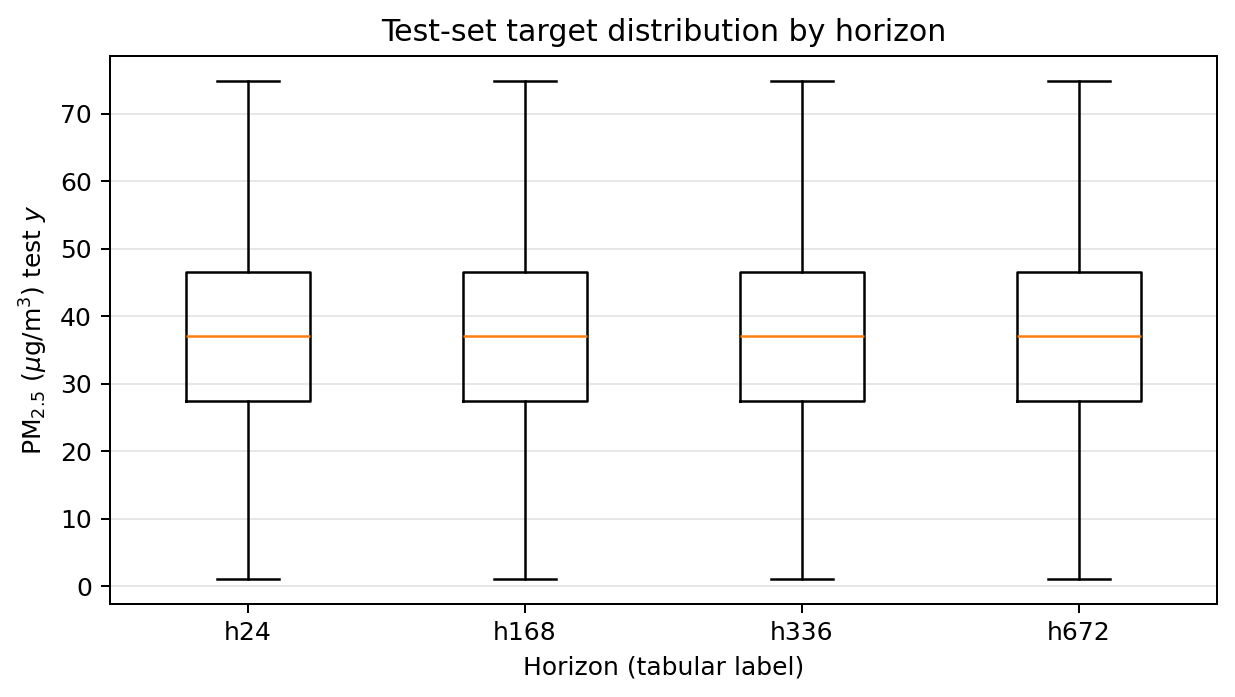
\includegraphics[width=0.60\textwidth]{figs/results_horizon_target_variability_box.png}%
%     \caption{Distribution of test-set forecast targets $y(t+H)$ by horizon (pooled 28-day test window). Identical boxplots reflect the same underlying test rows in this export, not necessarily equal difficulty at each $H$.}
%     \label{fig:horizon_variability}
% \end{figure}

% Forecasting performance was evaluated using three complementary metrics: Mean Absolute Error (MAE), Mean Squared Error (MSE), and the coefficient of determination ($R^2$). MAE measures the average magnitude of prediction errors and is expressed in the same unit as PM$_{2.5}$ concentration. MSE penalizes larger prediction errors more heavily through squared deviations, making it sensitive to extreme events. The $R^2$ metric quantifies the proportion of variability in observed PM$_{2.5}$ concentrations explained by the model.
% The evaluation metrics are defined as follows:

% \begin{equation}
% \text{MAE} =
% \frac{1}{n}
% \sum_{i=1}^{n}
% \left| y_i - \hat{y}_i \right|
% \label{eq:mae}
% \end{equation}

% \begin{equation}
% \text{MSE} =
% \frac{1}{n}
% \sum_{i=1}^{n}
% \left( y_i - \hat{y}_i \right)^2
% \label{eq:mse}
% \end{equation}

% \begin{equation}
% R^2 =
% 1 -
% \frac{
% \sum_{i=1}^{n}
% \left( y_i - \hat{y}_i \right)^2
% }{
% \sum_{i=1}^{n}
% \left( y_i - \bar{y} \right)^2
% }
% \label{eq:r2}
% \end{equation}

% where $y_i$ represents the observed PM$_{2.5}$ concentration, $\hat{y}_i$ denotes the predicted concentration, $\bar{y}$ is the mean observed concentration, and $n$ is the total number of observations.
% Because episodic pollution spikes carry substantial public health implications, additional stress testing was performed using upper-decile PM$_{2.5}$ events (MAE$^{90}$). This enabled evaluation of model robustness during hazardous pollution periods. To quantify uncertainty, block bootstrap confidence intervals were computed for model performance metrics. Paired statistical significance testing was additionally conducted on test-set prediction errors to determine whether performance differences between competing models were statistically significant.

% To enhance transparency and reproducibility, all data preprocessing, exploratory analyses, forecasting experiments, and statistical evaluations were implemented using open-source Python libraries. Model development employed widely used libraries, including \texttt{pandas}, \texttt{NumPy}, \texttt{scikit-learn}, \texttt{TensorFlow/Keras}, and \texttt{PyTorch}, where applicable. Chronological train–validation–test splitting was applied to prevent temporal leakage and ensure realistic forecasting conditions.
% All preprocessing decisions, feature engineering procedures, model hyperparameters, and evaluation protocols were documented to facilitate replication. Random seeds were fixed during model training to improve computational reproducibility. Consistent with open-science principles, the analytical workflow, trained model configurations, and non-sensitive processed data will be made publicly available upon publication to support transparency and future research on air quality forecasting in low-resource settings.

% \subsection{Data Collection and Study Setting}

% Air quality data were collected using the AirGradient Open Air monitor (Model O-1PST), an outdoor monitoring device measuring particulate matter (PM$_{2.5}$, PM$_1$, PM$_{10}$), particle number concentration (0.3~\textmu m), and co-located environmental variables including temperature, relative humidity, carbon dioxide (CO$_2$), total volatile organic compounds (TVOC), and a nitrogen oxides (NOX) index. Sensors were deployed at seven fixed sites in Tema, coastal Ghana, spanning industrial and residential micro-environments (including Tema Port, schools, and community sites). Observations were recorded hourly from 19 September 2025 to 15 February 2026.

% \subsection{Preprocessing and Regime Annotation}

% Raw data were aligned to a continuous hourly time axis in local time and cleaned to produce a corrected PM$_{2.5}$ target series for modelling. Short gaps in TVOC and NOX were imputed using time-ordered linear interpolation to preserve temporal continuity. Calendar fields (hour, day-of-week, month) were extracted from the local timestamp. We additionally annotate a simple Harmattan proxy as a date-based regime flag (pre-Harmattan vs Harmattan) to support stratified evaluation under the dominant seasonal shift in this region.

% \subsection{Supervised Forecasting Datasets}

% We study multi-horizon forecasting at horizons \(H \in \{24,168,336,672\}\) hours (24~h, 7~d, 14~d, 28~d). For a forecast origin time \(t\), the target is corrected PM$_{2.5}$ at label time \(t+H\). We evaluate two modelling paradigms.

% \subsubsection{Tabular direct-forecast datasets}

% For each horizon, we construct a supervised tabular dataset with one row per (site, origin time) and target \(y(t+H)\). Feature engineering uses only information available at or before time \(t\). Specifically, we generate:
% \begin{itemize}
%     \item lag features for the particulate and key environmental series (e.g., 1--48~h plus longer lags up to 168~h, and additional long lags where available),
%     \item rolling summary statistics (mean, standard deviation, max) computed on \emph{shifted} series (shift by 1) to avoid using the current hour in the window,
%     \item calendar features (hour, day-of-week, month),
%     \item Fourier terms on absolute time to represent daily (24~h) and weekly (168~h) seasonality,
%     \item one-hot encoding for site identity for pooled multi-site models.
% \end{itemize}

% \subsubsection{Sequence datasets (per-horizon and joint multi-horizon)}

% For sequence models, we construct input windows of length \(L\) hours ending at time \(t\), and predict corrected PM$_{2.5}$ at \(t+H\). The sequence feature tensor includes corrected pollutants and environmental covariates and is augmented with calendar encodings (sin/cos cyclic terms), Fourier terms, the Harmattan flag, and a location one-hot vector. We train two sequence variants:
% \begin{itemize}
%     \item \textbf{Per-horizon direct training}: one model per horizon trained on horizon-specific sequence datasets.
%     \item \textbf{Joint multi-horizon training}: one model outputs predictions for all horizons simultaneously (multi-output regression). To keep blocked splits leakage-safe across all horizons, the split key is the label time of the \emph{maximum} horizon.
% \end{itemize}

% \subsection{Models}

% \subsubsection{Baselines and classical machine learning}

% We include operational baselines based on persistence and seasonal recurrence using available lag features (e.g., weekly seasonal na\"{i}ve anchored at 168~h where applicable). As an interpretable statistical benchmark, we evaluate a restricted Ridge autoregressive model with PM$_{2.5}$ lags plus calendar/Fourier terms (``Ridge AR+Fourier''). We also fit classical machine learning models (linear SVR, Random Forest, XGBoost) on the same tabular feature matrices for each horizon.

% \subsubsection{LSTM sequence models and attention augmentation}

% We evaluate Long Short-Term Memory (LSTM) networks to model nonlinear temporal dynamics from multivariate input windows. The LSTM unit is defined by standard gating equations (Eqs.~\ref{equ1}--\ref{equ5}). We additionally test a multi-head attention augmentation that computes content-based reweighting over the sequence representation and fuses the attention summary with the LSTM representation and a pooled summary of the raw inputs. Figure~\ref{fig:architecture} summarises the two deep-learning setups: (left) per-horizon direct training with a single output head per model; (right) joint multi-horizon training with a shared encoder and multiple horizon outputs (with optional multi-head attention over the sequence).

% \begin{figure*}[t]
%     \centering
%     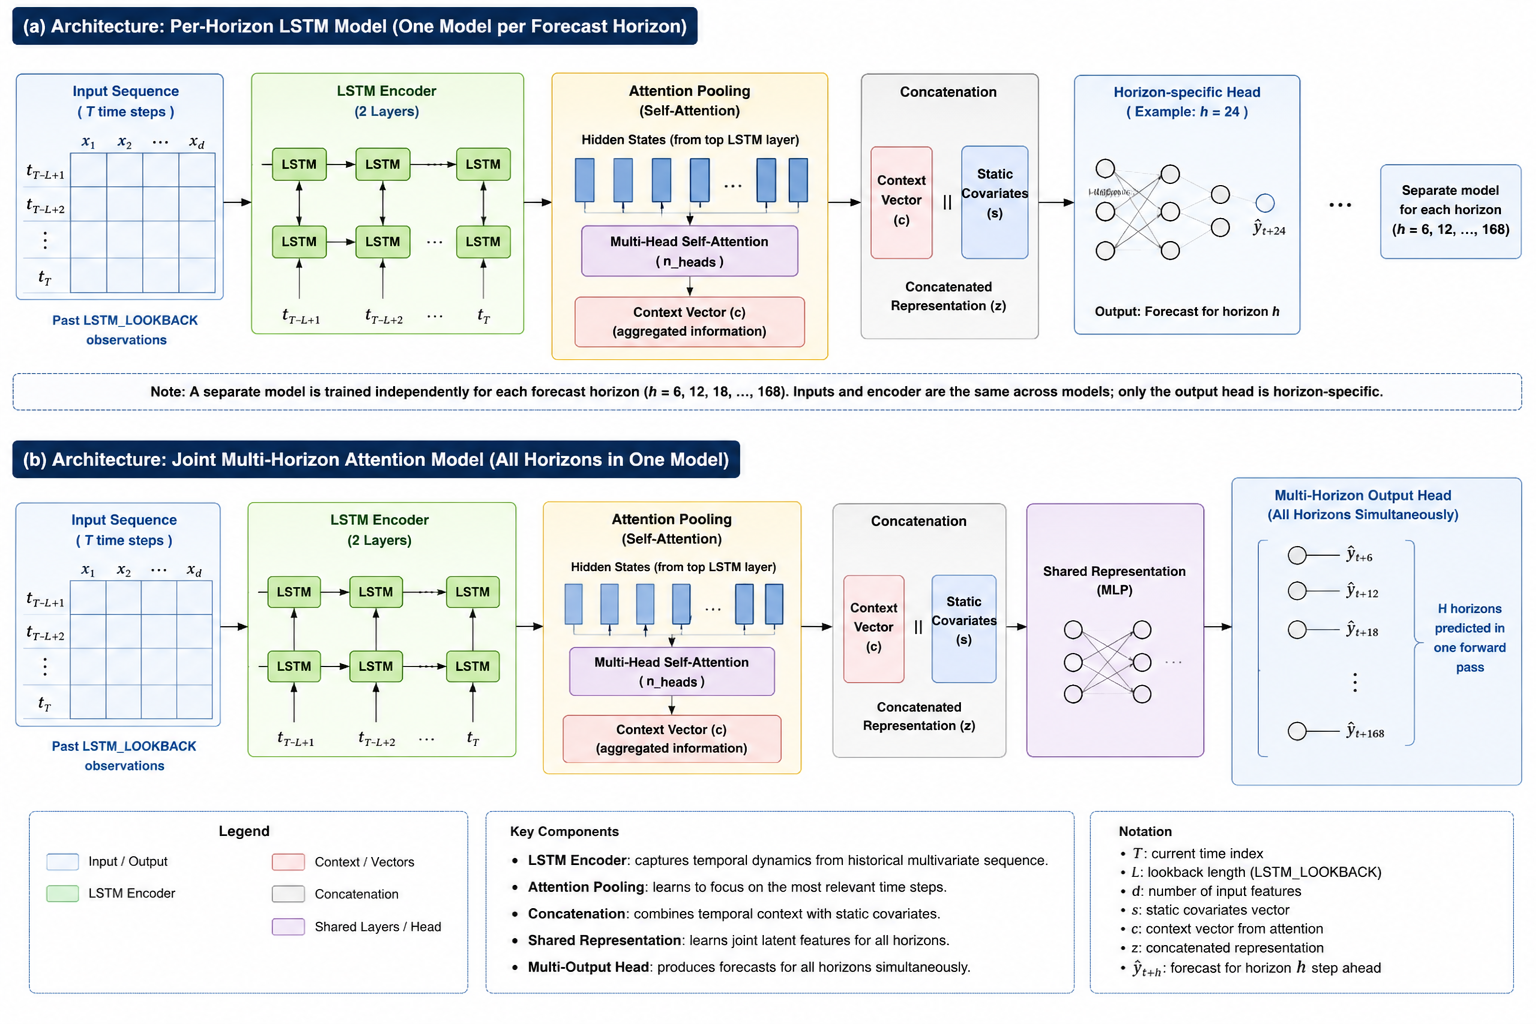
\includegraphics[width=0.92\textwidth]{figs/Architecture.png}%
%     \caption{Deep sequence model architectures. \textbf{(a)} Per-horizon direct forecasting: multivariate input window $\rightarrow$ LSTM encoder $\rightarrow$ optional multi-head attention pooling and fusion $\rightarrow$ dense head predicting PM$_{2.5}$ at one lead time $H$. \textbf{(b)} Joint multi-horizon training: shared representation predicts all horizons $\{24,168,336,672\}$~h simultaneously from one forward pass; splits are keyed to the maximum-horizon label time for leakage safety.}
%     \label{fig:architecture}
% \end{figure*}

% \begin{equation}
% i_t = \sigma \left( W_{x_i} x_t + W_{h_i} h_{t-1} + W_{c_i} c_{t-1} + b_i\right)
% \label{equ1}
% \end{equation}
% \begin{equation}
% f_t = \sigma\left(W_{x_f} x_t + W_{h_f} h_{t-1} + W_{c_f} c_{t-1} + b_f\right)
% \label{equ2}
% \end{equation}
% \begin{equation}
% c_t = f_t \odot c_{t-1} + i_t \odot \tanh\left(W_{x_c} x_t + W_{h_c} h_{t-1} + b_c\right)
% \label{equ3}
% \end{equation}
% \begin{equation}
% o_t = \sigma\left(W_{x_o} x_t + W_{h_o} h_{t-1} + W_{c_o} c_t + b_o\right)
% \label{equ4}
% \end{equation}
% \begin{equation}
% h_t = o_t \odot \tanh\left(c_t\right)
% \label{equ5}
% \end{equation}

% Importantly, the utility of attention in this study is contingent on training setup: in per-horizon direct training, attention does not consistently improve over vanilla LSTM, while in joint multi-horizon training it becomes the strongest-performing variant in our experiments (see Results).

% \subsection{Leakage-Safe Splits and Evaluation Metrics}

% All train/validation/test splits are defined by \emph{label time} (``target\_time'') using contiguous blocked windows, with the most recent segment reserved for testing. This prevents leakage that would occur if observations from the test label period influenced training through feature construction or random shuffling. Unless otherwise specified, we use a 14-day validation window and a 28-day held-out test window for pooled evaluation; for regime-stratified diagnostics we also compute an extended regime-spanning test window (84 days) so that both pre-Harmattan and Harmattan label times are represented.

% Models are evaluated using mean absolute error (MAE), root mean squared error (RMSE), and coefficient of determination (\(R^2\)). To stress-test performance on high-pollution events, we compute \textbf{upper-decile error} (MAE$^{90}$): MAE restricted to test rows whose observed PM$_{2.5}$ is at or above the 90th percentile of observed concentrations in the pooled test window. MAE$^{90}$ is reported alongside pooled MAE because public-health risk is driven disproportionately by tail hours, even when bulk accuracy appears acceptable. Where the test window spans both regimes, we also report regime-stratified metrics for pre-Harmattan versus Harmattan subsets.

% \subsubsection{Statistical uncertainty and paired comparisons}

% After each fitted model is evaluated on the held-out test window, we write one CSV per model and horizon under \texttt{reports/predictions/} with at least \texttt{target\_time}, \texttt{y\_true}, \texttt{y\_pred}, site/location, horizon, and model identifier (tabular and deep pipelines). These exports are the single source for bootstrap resampling and paired tests.

% We quantify uncertainty with a \textbf{moving-block bootstrap} on time-ordered test indices ($B{=}1000$ resamples; block length 168~h by default) to respect autocorrelation. We report bootstrap means and percentile 95\% confidence intervals for MAE, RMSE, and MAE$^{90}$ (script~12), merged into \texttt{results\_merged\_long.csv} (script~08) and reported in Table~\ref{tab:forecast-summary} and Figure~\ref{fig:forecast_mae}.

% We pre-specify a small set of \textbf{paired} comparisons on aligned rows (same \texttt{target\_time} and site; script~13): joint \texttt{mh\_lstm} vs per-horizon \texttt{lstm}; \texttt{mh\_lstm\_mha} vs \texttt{mh\_lstm}; and \texttt{mh\_lstm\_mha} vs Ridge AR+Fourier. For each pair we bootstrap the distribution of $\Delta$MAE (model~A minus model~B) using the same blocks and flag comparisons whose 95\% CI excludes zero (Table~\ref{tab:significance}). In the current export, statistically significant improvements ($\Delta$MAE CI excludes zero) are: \texttt{mh\_lstm\_mha} vs \texttt{mh\_lstm} at 7~d and 14~d, and \texttt{mh\_lstm\_mha} vs Ridge AR+Fourier at 28~d; all other pre-specified pairs in the table are non-significant or omitted. We tested multiple horizon--pair combinations; claims of significance are stated conservatively and should not be over-interpreted given the short record. Some joint-vs-per-horizon comparisons at short horizons are \emph{not} row-alignable because joint models use a single multi-horizon sequence split (label time keyed to the maximum horizon); those pairs are omitted from paired testing rather than forced.

% \subsubsection{Horizon target variability (14-day contextualisation)}

% To contextualise apparent ease of 14~d forecasting, we summarise test-set target distributions by horizon (script~15). On the pooled 28-day test window, marginal summaries of $y(t+H)$ are identical across $H$ when the same test row index set is used (Table~\ref{tab:horizon-variability}), so lower 14~d MAE should \emph{not} be interpreted as intrinsically lower target variance in this diagnostic alone. Figure~\ref{fig:horizon_variability} provides a visual check; definitive claims require horizon-specific label alignment and longer records.

% \subsubsection{Reproducibility}

% Training and evaluation are scripted in a public repository (commit pinned at submission). Deep models use TensorFlow/Keras with fixed random seeds; sequence construction, split boundaries, and exported prediction CSVs fully determine the reported metrics. Environment variables (\texttt{AIRP\_BATCH\_SIZE}, \texttt{AIRP\_TEST\_DAYS}, attention stride/head counts for multi-horizon runs) are documented in the repository README. Colab runs scripts 01--07 (feature construction through model training and prediction export); local runs merge metrics, bootstrap CIs, significance tests, and figures (scripts 08, 09, 11--13, 15).

% \begin{table}
% \centering
% \caption{Basic Statistics for Various Environmental Parameters}
% \resizebox{0.7500\textwidth}{!}{%
% % \begin{tabular}{lccccccccc}
% \begin{tabular}{llrrrrrr}
% \toprule
% Location & Parameter & Mean & Std & 25\% & 50\% (Median) & 75\% & Skewness \\
% \midrule

% \multirow{11}{*}{Divine Healer’s Church, Bethlehem}
% & PM$_{2.5}$ & 35.1507 & 20.4792 & 22.4 & 33.4 & 44.4 & 1.7861 \\
% & PM$_1$ & 21.7871 & 12.9154 & 12.2 & 21.8 & 28.6 & 1.1081 \\
% & PM$_{10}$ & 39.2128 & 22.8008 & 23.3 & 37.1 & 52.4 & 1.3309 \\
% & Particle Count & 1461.6865 & 924.1628 & 816.0 & 1253.0 & 1874.0 & 1.8027 \\
% & CO$_2$ & 543.7726 & 63.8664 & 501.0 & 542.0 & 580.0 & 0.4133 \\
% & Temperature & 28.2485 & 2.4634 & 26.5 & 27.5 & 30.1 & 0.6321 \\
% & Heat Index & 33.4196 & 5.2656 & 29.5 & 32.5 & 37.5 & 0.3953 \\
% & Humidity & 85.2387 & 8.8145 & 78.0 & 89.0 & 92.0 & -0.7973 \\
% & TVOC & 143.7646 & 138.3601 & 70.0 & 102.0 & 163.0 & 3.8437 \\
% & TVOC Index & 129.0867 & 81.2753 & 73.0 & 107.0 & 162.0 & 1.4666 \\
% & NOX Index & 1.1080 & 0.4254 & 1.0 & 1.0 & 1.0 & 5.3102 \\
% \midrule

% \multirow{11}{*}{Kpone Methodists School}
% & PM$_{2.5}$ & 20.7903 & 21.2845 & 2.75 & 18.7 & 30.6 & 3.2142 \\
% & PM$_1$ & 12.3342 & 12.5892 & 0.85 & 9.5 & 19.9 & 1.9575 \\
% & PM$_{10}$ & 22.6451 & 23.2542 & 2.95 & 19.5 & 33.2 & 2.8317 \\
% & Particle Count & 1274.5462 & 867.9515 & 682.5 & 1044.0 & 1645.5 & 2.3753 \\
% & CO$_2$ & 1125.1575 & 481.4314 & 731.5 & 947.0 & 1464.0 & 0.9101 \\
% & Temperature & 27.7575 & 1.6000 & 26.8 & 27.7 & 28.5 & 0.7838 \\
% & Heat Index & 32.9316 & 3.8173 & 30.8 & 33.2 & 35.1 & 0.1572 \\
% & Humidity & 89.0529 & 5.8500 & 87.0 & 90.0 & 93.0 & -1.3207 \\
% & TVOC & 163.3739 & 168.2272 & 70.0 & 113.0 & 192.0 & 3.6706 \\
% & TVOC Index & 139.6331 & 92.2967 & 73.0 & 117.0 & 182.0 & 1.2540 \\
% & NOX Index & 2.7539 & 16.5221 & 1.0 & 1.0 & 2.0 & 21.4757 \\
% \midrule

% \multirow{11}{*}{Satet International School, Tema Manhean}
% & PM$_{2.5}$ & 34.7627 & 26.2727 & 18.9 & 29.0 & 43.0 & 2.5693 \\
% & PM$_1$ & 21.9310 & 16.1668 & 10.5 & 19.6 & 28.5 & 1.9242 \\
% & PM$_{10}$ & 38.3854 & 28.6828 & 19.9 & 31.2 & 50.6 & 2.3234 \\
% & Particle Count & 1534.1690 & 1191.2897 & 770.0 & 1149.0 & 1904.5 & 2.3721 \\
% & CO$_2$ & 409.6265 & 8.7165 & 404.0 & 410.0 & 415.0 & 1.2237 \\
% & Temperature & 28.7937 & 2.0609 & 27.4 & 28.4 & 30.5 & 0.2829 \\
% & Heat Index & 35.1443 & 4.7276 & 32.0 & 34.8 & 38.85 & 0.0125 \\
% & Humidity & 84.9601 & 7.0012 & 79.0 & 87.0 & 90.0 & -0.5559 \\
% & TVOC & 156.0372 & 161.8372 & 64.0 & 105.0 & 184.0 & 3.9079 \\
% & TVOC Index & 133.3449 & 91.1555 & 66.0 & 108.0 & 176.0 & 1.2940 \\
% & NOX Index & 1.1861 & 0.8014 & 1.0 & 1.0 & 1.0 & 13.0968 \\
% \midrule

% \multirow{11}{*}{Tema Community 25 Estate}
% & PM$_{2.5}$ & 19.1187 & 12.3902 & 10.8 & 16.1 & 25.6 & 1.6759 \\
% & PM$_1$ & 18.9518 & 10.5298 & 10.3 & 19.3 & 25.9 & 0.6779 \\
% & PM$_{10}$ & 33.0528 & 17.8615 & 20.5 & 30.5 & 45.3 & 0.8436 \\
% & Particle Count & 1241.2735 & 706.4633 & 742.0 & 1064.0 & 1588.0 & 1.6528 \\
% & CO$_2$ & 521.4981 & 50.3581 & 488.0 & 517.0 & 544.0 & 1.2160 \\
% & Temperature & 28.2471 & 2.1503 & 26.9 & 27.8 & 29.6 & 0.6072 \\
% & Heat Index & 33.1704 & 4.3064 & 30.6 & 32.9 & 36.0 & 0.2057 \\
% & Humidity & 83.8868 & 8.6199 & 77.0 & 87.0 & 91.0 & -0.7878 \\
% & TVOC & 141.8982 & 129.2846 & 76.0 & 105.0 & 159.0 & 4.0268 \\
% & TVOC Index & 130.0163 & 77.1320 & 80.0 & 110.0 & 159.0 & 1.6103 \\
% & NOX Index & 1.1621 & 0.5146 & 1.0 & 1.0 & 1.0 & 4.1715 \\
% \midrule

% \multirow{11}{*}{Tema Community 3 SSNIT Flat}
% & PM$_{2.5}$ & 24.8065 & 20.9875 & 8.1 & 21.8 & 35.925 & 2.4092 \\
% & PM$_1$ & 15.0189 & 13.2838 & 4.1 & 11.6 & 23.6 & 1.5065 \\
% & PM$_{10}$ & 27.4233 & 23.4506 & 8.5 & 22.6 & 40.8 & 2.0445 \\
% & Particle Count & 1040.5761 & 866.2836 & 451.75 & 776.0 & 1371.75 & 2.6291 \\
% & CO$_2$ & 576.1674 & 103.0334 & 501.75 & 558.0 & 632.0 & 0.9370 \\
% & Temperature & 28.1589 & 1.8527 & 26.9 & 27.9 & 29.4 & 0.2266 \\
% & Heat Index & 33.6989 & 4.4620 & 30.8 & 33.5 & 36.7 & 0.0403 \\
% & Humidity & 86.8197 & 6.3862 & 82.0 & 88.0 & 92.0 & -0.4383 \\
% & TVOC & 158.1219 & 174.1002 & 65.0 & 102.0 & 188.0 & 3.8773 \\
% & TVOC Index & 135.2513 & 95.5831 & 68.0 & 107.0 & 182.0 & 1.2931 \\
% & NOX Index & 1.3472 & 0.8285 & 1.0 & 1.0 & 1.0 & 4.8093 \\
% \midrule

% \multirow{11}{*}{Tema Community 7, Royal School}
% & PM$_{2.5}$ & 28.3864 & 19.7791 & 14.3 & 26.7 & 38.3 & 2.5316 \\
% & PM$_1$ & 17.4160 & 12.6373 & 6.8 & 16.7 & 25.2 & 1.3593 \\
% & PM$_{10}$ & 31.6907 & 22.3319 & 15.3 & 28.0 & 44.6 & 2.0604 \\
% & Particle Count & 1193.6866 & 859.0131 & 605.0 & 963.0 & 1548.0 & 2.5052 \\
% & CO$_2$ & 460.9066 & 31.0177 & 437.0 & 460.0 & 477.0 & 0.6816 \\
% & Temperature & 28.3482 & 2.1615 & 26.9 & 27.8 & 30.0 & 0.5604 \\
% & Heat Index & 33.7408 & 4.5352 & 31.0 & 33.4 & 37.3 & 0.1166 \\
% & Humidity & 85.2396 & 8.5591 & 79.0 & 89.0 & 92.0 & -0.8140 \\
% & TVOC & 155.6156 & 150.9939 & 74.0 & 111.0 & 182.0 & 3.8927 \\
% & TVOC Index & 137.0143 & 86.1431 & 77.0 & 115.0 & 177.0 & 1.3166 \\
% & NOX Index & 1.2561 & 0.7109 & 1.0 & 1.0 & 1.0 & 3.6172 \\
% \midrule

% \multirow{11}{*}{Tema Port}
% & PM$_{2.5}$ & 25.7750 & 16.7039 & 12.7 & 23.6 & 36.0 & 1.1372 \\
% & PM$_1$ & 16.0620 & 11.3525 & 6.6 & 13.8 & 24.0 & 0.9534 \\
% & PM$_{10}$ & 28.6979 & 19.3024 & 13.5 & 24.8 & 40.9 & 0.9996 \\
% & Particle Count & 1120.3803 & 741.3476 & 604.0 & 911.0 & 1446.0 & 1.7759 \\
% & CO$_2$ & 465.8182 & 24.4599 & 449.0 & 463.0 & 481.0 & 0.8227 \\
% & Temperature & 29.0394 & 1.9365 & 27.8 & 28.7 & 30.3 & 0.3989 \\
% & Heat Index & 35.7426 & 4.4853 & 32.9 & 35.4 & 38.7 & 0.1167 \\
% & Humidity & 84.0947 & 6.2794 & 80.0 & 86.0 & 89.0 & -0.7249 \\
% & TVOC & 150.3369 & 152.3300 & 68.0 & 103.0 & 176.0 & 3.9675 \\
% & TVOC Index & 130.8572 & 86.2846 & 70.0 & 107.0 & 170.5 & 1.3079 \\
% & NOX Index & 1.1991 & 0.7203 & 1.0 & 1.0 & 1.0 & 11.7325 \\
% \bottomrule
% \end{tabular}}
% \label{tab:timeseries-data}
% \end{table}

% Table~\ref{tab:timeseries-data} summarises the hourly observations and highlights clear spatial heterogeneity across monitoring locations. Mean PM$_{2.5}$ concentrations range from approximately 19 to 35 µg/m$^3$, consistently exceeding WHO guideline levels. Particulate variables exhibit pronounced positive skewness, indicating episodic high-concentration events rather than symmetric variability. NOX and TVOC show extreme skewness at selected sites, suggesting intermittent but intense emission episodes. In contrast, meteorological variables display lower dispersion and more stable distributions; humidity is mildly negatively skewed, while temperature remains relatively symmetric. These patterns indicate that pollutant dynamics are shaped primarily by episodic emissions and seasonal forcing, with strong localized source effects.





\section{Results}\label{sec3}
\subsection{Environmental and exposure characteristics}

PM$_{2.5}$ concentrations exhibited substantial spatial and temporal variability across the monitoring network. Mean concentrations ranged from 19.12~$\mu$g\,m$^{-3}$ at Tema Community 25 Estate to 35.15~$\mu$g\,m$^{-3}$ at Divine Healer's Church, Bethlehem. Satet International School also recorded a high mean concentration of 34.76~$\mu$g\,m$^{-3}$, while concentrations at Tema Port, Tema Community 3 SSNIT Flats and Tema Community 7 were generally between 24 and 29~$\mu$g\,m$^{-3}$. The distributions were positively skewed at all sites, with skewness ranging from 1.14 to 3.21, indicating the occurrence of episodic high-concentration events.
\begin{table}[htbp]
\centering
\caption{PM$_{2.5}$ exposure burden, ratio to WHO guideline \citep{world2021global} exceedances and site-category averages across monitoring locations in coastal Greater Accra, Ghana. The monitoring period covered approximately six months; this comparison is descriptive and should not be interpreted as an annual exposure assessment.}
\label{tab:exposure_spatial}
\resizebox{0.98\textwidth}{!}{%
\begin{tabular}{llcccc}
\toprule
Category & Site &
Mean PM$_{2.5}$ &
Annual Guideline Ratio &
Daily Guideline Ratio &
Exceedance (\%) \\
&
&
($\mu$g m$^{-3}$) &
(5 $\mu$g m$^{-3}$) &
(15 $\mu$g m$^{-3}$) &
$>$15 $\mu$g m$^{-3}$ \\
\midrule

Industrial &
Tema Port &
25.77 &
5.15 &
1.72 &
69.83 \\
\cmidrule(lr){2-6}
&
\textbf{Category Mean} &
\textbf{25.77} &
\textbf{5.15} &
\textbf{1.72} &
\textbf{69.83} \\
\midrule
Residential &
Divine Healer's Church, Bethlehem &
35.15 &
7.03 &
2.34 &
85.68 \\
&
Tema Community 25 Estate &
19.12 &
3.82 &
1.27 &
55.00 \\
&
Tema Community 3 SSNIT Flat &
24.81 &
4.96 &
1.65 &
62.04 \\
\cmidrule(lr){2-6}
&
\textbf{Category Mean} &
\textbf{26.36} &
\textbf{5.27} &
\textbf{1.75} &
\textbf{67.57} \\
\midrule
School &
Satet International School &
34.76 &
6.95 &
2.32 &
81.33 \\
&
Tema Community 7 (Royal School) &
28.39 &
5.68 &
1.89 &
74.06 \\
&
Kpone Methodist School &
20.79 &
4.16 &
1.39 &
56.80 \\
\cmidrule(lr){2-6}
&
\textbf{Category Mean} &
\textbf{27.98} &
\textbf{5.60} &
\textbf{1.87} &
\textbf{70.73} \\
\midrule
\multicolumn{2}{l}{\textbf{Overall Mean}} &
\textbf{26.95} &
\textbf{5.39} &
\textbf{1.80} &
\textbf{69.25} \\
\bottomrule
\end{tabular}}
\end{table}

Exposure levels were elevated across all monitoring environments. Approximately 69.25\% of observations exceeded the WHO daily PM$_{2.5}$ guideline of 15~$\mu$g\,m$^{-3}$ (Table~\ref{tab:exposure_spatial}). Exceedance rates varied from 55.00\% at Tema Community 25 Estate to 85.68\% at Divine Healer's Church. When sites were grouped by land-use category, school locations recorded the highest category-average concentration (27.98~$\mu$g\,m$^{-3}$), followed by residential locations (26.36~$\mu$g\,m$^{-3}$) and Tema Port (25.77~$\mu$g\,m$^{-3}$).
Hourly concentrations also showed a clear diurnal pattern (Figure~\ref{fig:diurnal}). PM$_{2.5}$ increased during the early morning and reached its highest concentrations between 05:00 and 07:00, with a pooled mean of approximately 48~$\mu$g\,m$^{-3}$ around 06:00. Concentrations declined towards midday, reaching their lowest levels between approximately 13:00 and 14:00, before increasing again during the evening.
\begin{figure}
    \centering
    \begin{subfigure}{0.48\textwidth}
        \centering    \includegraphics[width=\linewidth]{eda_diurnal_curve_pooled.png}%
        \caption{Pooled hourly profile (mean, median, and interquartile band).}%
        \label{fig:diurnal_pooled}
    \end{subfigure}\hfill
    \begin{subfigure}{0.48\textwidth}
        \centering
        \includegraphics[width=\linewidth]{eda_diurnal_curve_by_regime.png}%
        \caption{Median diurnal curves stratified by Harmattan versus pre-Harmattan conditions.}%
        \label{fig:diurnal_regime}
    \end{subfigure}
    \caption{Diurnal variation in corrected PM$_{2.5}$ on local time (all sites pooled).}
    \label{fig:diurnal}
\end{figure}

\orig{The grouped predictor analysis further showed that historical PM$_{2.5}$ information provided the largest contribution to prediction, accounting for 27.64\% of total importance (Table~\ref{tab:drivers}). Particulate indicators contributed 22.12\%, followed by temporal indicators (15.78\%), meteorological conditions (10.40\%), spatial factors (8.12\%), CO$_2$ (6.63\%), and other environmental variables (9.31\%). The dominance of lagged PM$_{2.5}$ and particulate indicators indicates substantial temporal persistence in the observed pollution series.}
\prop{Grouped permutation importance on the 24-h Random Forest (validation block; $R=8$ joint shuffles per family) showed that lagged and rolling PM$_{2.5}$ was the only family whose removal raised MAE by a large, stable amount ($\Delta$MAE $=0.74$~$\mu$g\,m$^{-3}$; 5th--95th percentile 0.60--0.91; Table~\ref{tab:drivers-prop}). Meteorology contributed 0.25 (0.17--0.31) and CO$_2$ 0.10 (0.05--0.17). Site and calendar/Fourier terms were small. Other particulate lags (PM$_1$, PM$_{10}$, 0.3~$\mu$m counts) had a \emph{negative} permutation $\Delta$MAE ($-0.19$), i.e.\ shuffling them did not hurt and slightly helped, while impurity importance assigned that family 41\% of MDI because those columns are collinear with PM$_{2.5}$ history. These $\Delta$MAE values are predictive contributions on one validation window rather than causal source shares.}
{\color{blue}
\begin{table}[htbp]
\centering
\caption{Grouped predictor importance and environmental interpretation of PM$_{2.5}$ drivers. Predictor importance is interpreted as predictive contribution and should not be regarded as evidence of causal source attribution.}
\label{tab:drivers}
\resizebox{0.950\textwidth}{!}{%
\begin{tabular}{lcc}
\toprule
Driver Category & Importance (\%) & Potential Environmental Interpretation \\
\midrule
Particulate indicators
(0.3, PM$_{1.0}$, PM$_{10}$) & 22.12 &
Aerosol persistence and particle accumulation \\
Meteorological conditions
(temperature, humidity) & 10.40 &
Atmospheric dispersion and particle hygroscopic growth \\
Combustion proxy
(CO$_2$) & 6.63 &
Potential spatial differences in local environmental and land-use conditions \\
Temporal indicators
(hour, day, month, season) & 15.78 &
Human activity patterns and seasonal cycles \\
Lagged PM$_{2.5}$ metrics
(24 h, 7 d, 14 d, 28 d) & 27.64 &
Pollution persistence and atmospheric memory \\
Spatial factors
(site/location) & 8.12 &
Local source characteristics and land-use differences \\
Other environmental variables & 9.31 &
Residual environmental influences \\
\bottomrule
\end{tabular}}
\end{table}
}
{\color{red}
\begin{table}[htbp]
\centering
\caption{Grouped permutation importance for the 24-h Random Forest on the validation block ($R=8$). $\Delta$MAE is the increase in MAE after jointly permuting that family (mean and 5th--95th percentiles). Positive MDI shares are shown only as a collinearity check. Not causal attribution.}
\label{tab:drivers-prop}
\resizebox{0.98\textwidth}{!}{%
\begin{tabular}{lrrrr}
\toprule
Family & $n$ cols & $\Delta$MAE mean & 5th--95th pct.\ & MDI share (\%) \\
\midrule
Lagged / rolling PM$_{2.5}$ & 70 & 0.74 & 0.60--0.91 & 25.8 \\
Meteorological conditions & 142 & 0.25 & 0.17--0.31 & 16.4 \\
Combustion proxy (CO$_2$) & 71 & 0.10 & 0.05--0.17 & 9.1 \\
Spatial (site) & 7 & 0.02 & 0.01--0.02 & 0.2 \\
Temporal / Fourier & 16 & 0.01 & 0.00--0.02 & 5.1 \\
Other environmental & 1 & 0.00 & $-0.01$--0.02 & 2.1 \\
Particulate indicators (PM$_1$, PM$_{10}$, 0.3~$\mu$m) & 213 & $-0.19$ & $-0.30$--$-0.08$ & 41.5 \\
\bottomrule
\end{tabular}}
\end{table}
}


\subsection{\orig{Harmattan as an environmental regime shift}\prop{Harmattan as a calendar-defined atmospheric period}}

Harmattan conditions were associated with a clear shift in the distribution of PM$_{2.5}$ concentrations (Table~\ref{tab:harmattan}). \orig{Mean PM$_{2.5}$ increased from 25.77~$\mu$g\,m$^{-3}$ during the pre-Harmattan period to 31.19~$\mu$g\,m$^{-3}$ during Harmattan, corresponding to an increase of approximately 21\%.} \prop{Under the calendar definition in Section~2 (pre-Harmattan: through 30~November~2025; Harmattan: 1~December~2025--28~February~2026), mean PM$_{2.5}$ increased from 25.77~$\mu$g\,m$^{-3}$ to 31.19~$\mu$g\,m$^{-3}$, corresponding to an increase of approximately 21\%.} Median concentrations similarly increased from 22.90 to 27.20~$\mu$g\,m$^{-3}$, while the 95th percentile increased from 59.87 to 63.40~$\mu$g\,m$^{-3}$.
The regime difference was also evident in the diurnal profiles (Figure~\ref{fig:diurnal}). During Harmattan, median PM$_{2.5}$ concentrations remained elevated throughout the day. Midday concentrations were approximately 23--26~$\mu$g\,m$^{-3}$ compared with 8--12~$\mu$g\,m$^{-3}$ during the pre-Harmattan period. Early-morning concentrations also increased, reaching approximately 50~$\mu$g\,m$^{-3}$ during Harmattan compared with approximately 36~$\mu$g\,m$^{-3}$ before Harmattan.

These distributional changes demonstrate a marked shift in PM$_{2.5}$ conditions between the pre-Harmattan and Harmattan periods and provide the basis for the subsequent regime-specific forecast evaluation.
\begin{table}[htbp]
\centering
\caption{Comparison of PM$_{2.5}$ characteristics and forecasting performance between pre-Harmattan and Harmattan periods. PM$_{2.5}$ statistics were computed from corrected observations across all monitoring sites. Forecast MAEs are based on the regime-stratified Random Forest model, which achieved the lowest error across most forecasting horizons on the extended test window.}
\label{tab:harmattan}
\begin{tabular}{lcc}
\toprule
\textbf{Metric} & \textbf{Pre-Harmattan} & \textbf{Harmattan} \\
\midrule
Mean PM$_{2.5}$ ($\mu$g m$^{-3}$) & 25.77 & 31.19 \\
Median PM$_{2.5}$ ($\mu$g m$^{-3}$) & 22.90 & 27.20 \\
95th Percentile PM$_{2.5}$ ($\mu$g m$^{-3}$) & 59.87 & 63.40 \\
Standard Deviation ($\mu$g m$^{-3}$) & 21.05 & 19.83 \\
\midrule
24-h Forecast MAE ($\mu$g m$^{-3}$) & 7.89 & 10.61 \\
7-day Forecast MAE ($\mu$g m$^{-3}$) & 8.56 & 12.78 \\
14-day Forecast MAE ($\mu$g m$^{-3}$) & 9.85 & 12.44 \\
28-day Forecast MAE ($\mu$g m$^{-3}$) & 10.86 & 14.87 \\
\midrule
Mean Forecast MAE ($\mu$g m$^{-3}$) & 9.29 & 12.68 \\
Relative Increase in MAE (\%) & -- & 36.4 \\
\bottomrule
\end{tabular}
\end{table}

\subsection{Multi-horizon forecasting performance}

Forecasting performance varied substantially with model class and prediction horizon (Table~\ref{tab:forecast-summary}; Figure~\ref{fig:forecast_mae}). Model rankings were not constant across horizons, indicating that increasing model complexity did not provide a uniform forecasting advantage.
\prop{Joint models used 1{,}374 training and 1{,}957 test sequences; tabular models used 13{,}263--17{,}285 training rows and 4{,}037 test rows. Unpaired MAE comparisons across families are therefore not sample-size matched (Table~\ref{tab:eval-splits-prop}).}
\begin{table}[H]
\centering
\caption{Representative out-of-sample forecasting accuracy on pooled multi-site test splits (corrected PM$_{2.5}$, $\mu$g/m$^3$). \texttt{mh\_lstm} / \texttt{mh\_lstm\_mha} are jointly trained multi-horizon sequence models. MAE 95\% CI: moving-block bootstrap on exported test predictions ($B{=}1000$, block length 168~h).}
\label{tab:forecast-summary}
\resizebox{\textwidth}{!}{%
\begin{tabular}{llrrrr}
\toprule
Horizon & Model & MAE & MAE 95\% CI & RMSE & $R^2$ \\
\midrule
24~h & Ridge AR+Fourier & 11.96 & [10.96, 12.98] & 18.22 & 0.210 \\
24~h & Joint multi-horizon LSTM (\texttt{mh\_lstm}) & 12.31 & [9.99, 14.59] & 19.23 & 0.028 \\
24~h & Joint multi-horizon LSTM + attention (\texttt{mh\_lstm\_mha}) & 12.94 & [10.66, 14.87] & 18.30 & 0.120 \\
24~h & Seasonal naïve (24h anchor) & 13.76 & [12.24, 15.10] & 21.94 & $-0.144$ \\
24~h & Random Forest (tabular lags) & 14.09 & [12.62, 15.58] & 18.97 & 0.144 \\
24~h & Linear SVR (tabular lags) & 20.10 & [18.47, 22.09] & 26.17 & $-0.629$ \\
24~h & XGBoost (tabular lags) & 22.16 & [19.63, 24.66] & 27.07 & $-0.743$ \\
24~h & LSTM (per-horizon direct) & 23.19 & [19.92, 27.08] & 30.24 & $-1.344$ \\
\midrule
7~d (168~h) & Joint multi-horizon LSTM + attention (\texttt{mh\_lstm\_mha}) & 11.32 & [9.68, 12.92] & 17.94 & 0.155 \\
7~d (168~h) & LSTM (per-horizon direct) & 13.04 & [11.92, 14.05] & 18.80 & 0.207 \\
7~d (168~h) & Joint multi-horizon LSTM (\texttt{mh\_lstm}) & 15.02 & [12.75, 16.59] & 21.55 & $-0.219$ \\
7~d (168~h) & Seasonal naïve (weekly anchor) & 15.39 & [13.40, 17.23] & 22.74 & $-0.226$ \\
7~d (168~h) & Random Forest (tabular lags) & 19.08 & [15.83, 22.55] & 24.29 & $-0.403$ \\
7~d (168~h) & Linear SVR (tabular lags) & 37.21 & [35.18, 39.25] & 41.14 & $-3.027$ \\
7~d (168~h) & XGBoost (tabular lags) & 43.46 & [36.69, 51.23] & 50.93 & $-5.171$ \\
\midrule
14~d (336~h) & Joint multi-horizon LSTM + attention (\texttt{mh\_lstm\_mha}) & 9.78 & [8.69, 10.80] & 16.58 & 0.108 \\
14~d (336~h) & LSTM (per-horizon direct) & 14.31 & [12.70, 15.72] & 21.41 & $-0.011$ \\
14~d (336~h) & Linear SVR (tabular lags) & 14.52 & [12.57, 16.27] & 19.49 & 0.096 \\
14~d (336~h) & Ridge AR+Fourier & 15.39 & [13.48, 17.17] & 20.31 & 0.019 \\
14~d (336~h) & Joint multi-horizon LSTM (\texttt{mh\_lstm}) & 16.58 & [14.72, 18.45] & 22.00 & $-0.571$ \\
\textcolor{red}{14~d (336~h)} & \textcolor{red}{Seasonal naïve (14d anchor)} & \textcolor{red}{18.88} & \textcolor{red}{[17.57, 20.36]} & \textcolor{red}{25.54} & \textcolor{red}{$-0.535$} \\
14~d (336~h) & Random Forest (tabular lags) & 19.64 & [16.31, 22.96] & 25.47 & $-0.543$ \\
14~d (336~h) & XGBoost (tabular lags) & 24.88 & [20.77, 29.19] & 31.73 & $-1.395$ \\
\midrule
28~d (672~h) & Joint multi-horizon LSTM + attention (\texttt{mh\_lstm\_mha}) & 13.56 & [11.25, 16.35] & 19.98 & 0.041 \\
28~d (672~h) & Joint multi-horizon LSTM (\texttt{mh\_lstm}) & 14.92 & [13.41, 16.76] & 21.37 & $-0.097$ \\
28~d (672~h) & Ridge AR+Fourier & 15.48 & [14.16, 16.78] & 21.02 & $-0.051$ \\
28~d (672~h) & Random Forest (tabular lags) & 15.62 & [13.26, 17.85] & 21.38 & $-0.088$ \\
28~d (672~h) & XGBoost (tabular lags) & 19.25 & [16.33, 22.33] & 25.41 & $-0.536$ \\
28~d (672~h) & Linear SVR (tabular lags) & 23.48 & [20.83, 26.37] & 28.28 & $-0.902$ \\
28~d (672~h) & Seasonal naïve (28d anchor) & 17.99 & [16.65, 19.60] & 25.17 & $-0.507$ \\
\bottomrule
\end{tabular}}
\end{table}

At the 24-h horizon, Ridge AR+Fourier achieved the lowest MAE of 11.96~$\mu$g\,m$^{-3}$ (95\% CI: 10.96--12.98), with an RMSE of 18.22~$\mu$g\,m$^{-3}$ and $R^2=0.210$. The joint multi-horizon LSTM achieved a comparable MAE of 12.31~$\mu$g\,m$^{-3}$, while the attention-enhanced joint LSTM recorded an MAE of 12.94~$\mu$g\,m$^{-3}$. The seasonal-na\"ive and Random Forest models produced MAEs of 13.76 and 14.09~$\mu$g\,m$^{-3}$, respectively. In contrast, the direct per-horizon LSTM recorded an MAE of 23.19~$\mu$g\,m$^{-3}$ and $R^2=-1.344$. \prop{A 24-h lookback and width check (Table~\ref{tab:lstm-h24-sens}) supported retention of the $L=168$~h, 64-unit architecture used for this score. A residual 24-h LSTM diagnostic for this setting is reported in Section~\ref{sec:diagnostics}.}
\begin{figure}
    \centering    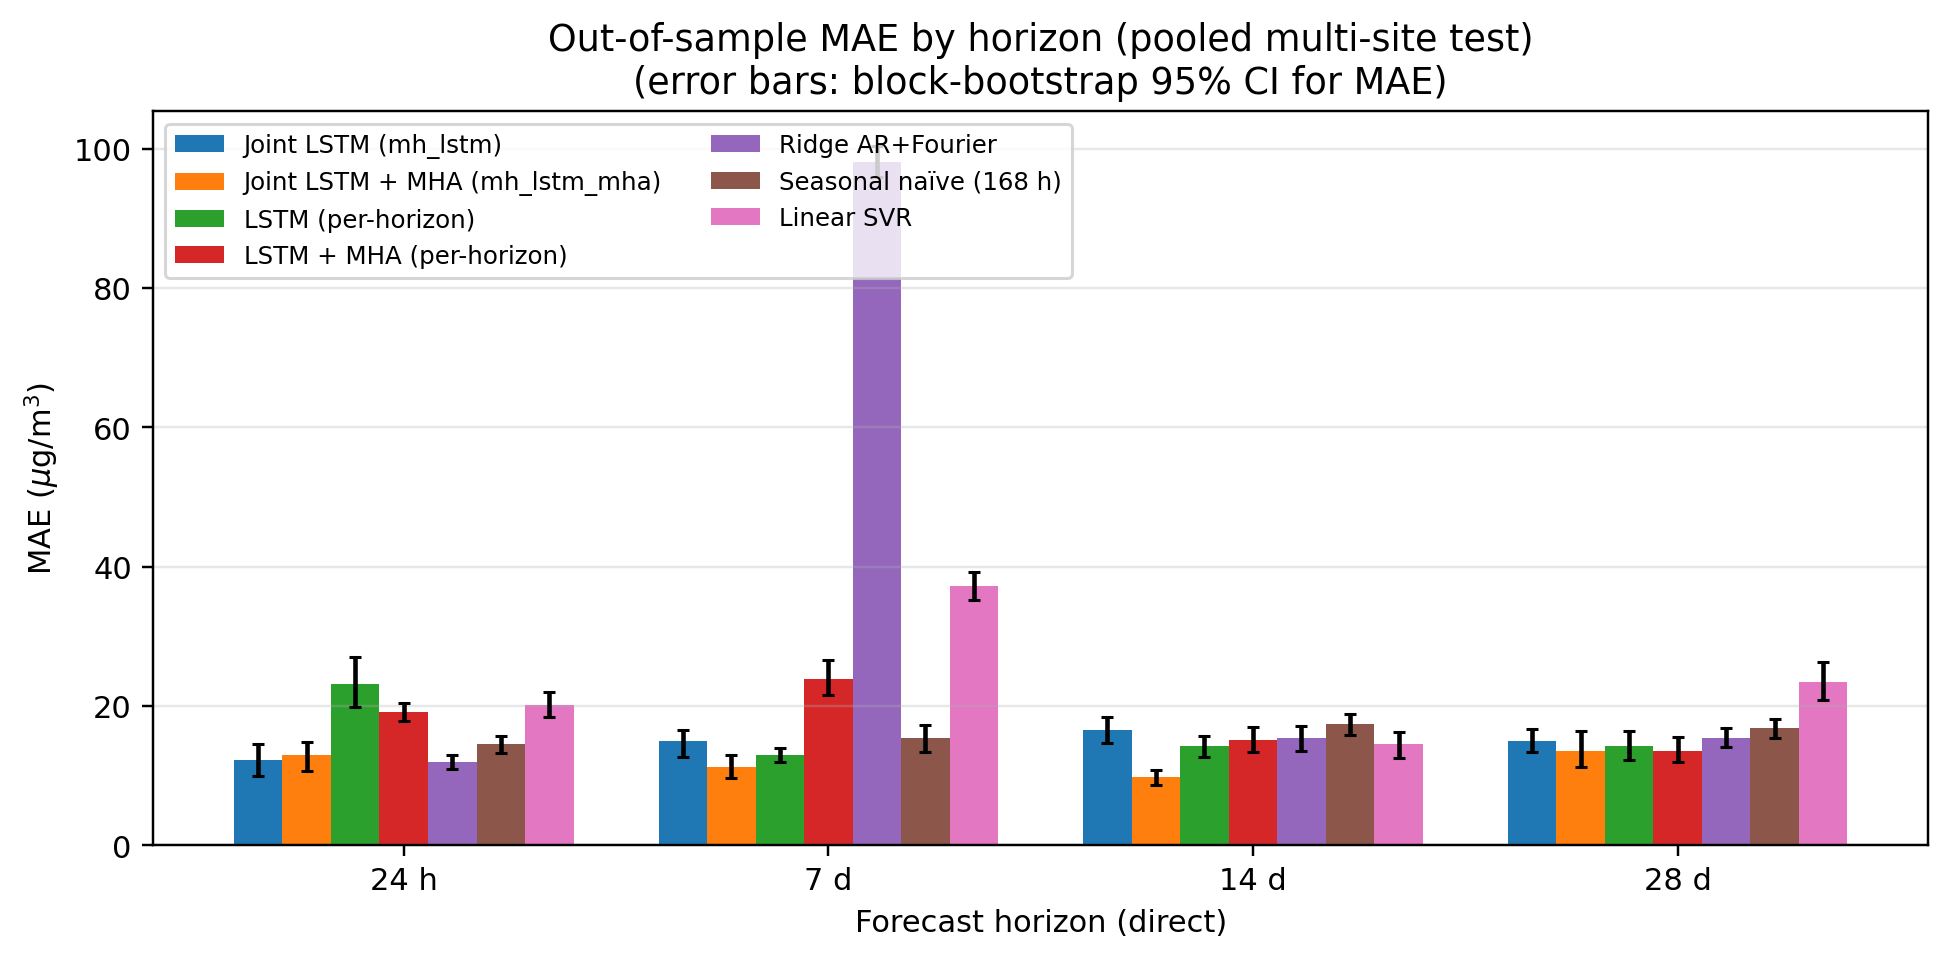
\includegraphics[width=0.82\textwidth]{figs/results_mae_by_horizon.png}%
    \caption{Mean absolute error (MAE; $\mu$g/m$^3$) on pooled multi-site test windows for selected models, shown by direct forecasting horizon. Error bars denote 95\% percentile intervals from a moving-block bootstrap ($B{=}1000$, block length 168~h) on time-ordered test rows.}
    \label{fig:forecast_mae}
\end{figure}

At 7 days, the ranking changed in favour of the attention-enhanced sequence model. The joint LSTM with attention achieved the lowest MAE of 11.32~$\mu$g\,m$^{-3}$ (95\% CI: 9.68--12.92), compared with 13.04~$\mu$g\,m$^{-3}$ for the direct LSTM, 15.02~$\mu$g\,m$^{-3}$ for the joint LSTM without attention, and 15.39~$\mu$g\,m$^{-3}$ for the seasonal-na\"ive benchmark. Random Forest, Linear SVR and XGBoost recorded higher MAEs of 19.08, 37.21 and 43.46~$\mu$g\,m$^{-3}$, respectively.

\orig{The advantage of the attention-enhanced model was most pronounced at the 14-day horizon. Joint LSTM with attention achieved an MAE of 9.78~$\mu$g\,m$^{-3}$ (95\% CI: 8.69--10.80), an RMSE of 16.58~$\mu$g\,m$^{-3}$ and $R^2=0.108$. The next-lowest errors were obtained by the direct LSTM (14.31~$\mu$g\,m$^{-3}$) and Linear SVR (14.52~$\mu$g\,m$^{-3}$). Ridge AR+Fourier, joint LSTM without attention, Random Forest, and XGBoost produced MAEs of 15.39, 16.58, 19.64, and 24.88~$\mu$g\,m$^{-3}$, respectively.}
\prop{The advantage of the attention-enhanced model was most pronounced at the 14-day horizon. Joint LSTM with attention achieved an MAE of 9.78~$\mu$g\,m$^{-3}$ (95\% CI: 8.69--10.80), an RMSE of 16.58~$\mu$g\,m$^{-3}$ and $R^2=0.108$. The next-lowest errors were obtained by the direct LSTM (14.31~$\mu$g\,m$^{-3}$) and Linear SVR (14.52~$\mu$g\,m$^{-3}$). Ridge AR+Fourier, joint LSTM without attention, seasonal na\"ive (14-day origin lag), Random Forest, and XGBoost produced MAEs of 15.39, 16.58, 18.88, 19.64, and 24.88~$\mu$g\,m$^{-3}$, respectively.}

\prop{This 14-day MAE was also lower than the same attention model's 24-h (12.94; 95\% CI: 10.66--14.87) and 7-day (11.32; 95\% CI: 9.68--12.92) errors, so the error--horizon relationship was non-monotonic. The 14-day MAE interval was separated from the 24-h interval but overlapped the 7-day interval, so the 14- versus 7-day dip is a point-estimate pattern rather than a strongly separated contrast. The lower 14-day MAE therefore does not imply that 14-day PM$_{2.5}$ is intrinsically easier to forecast: $R^2$ was higher at 7 days (0.155) than at 14 days (0.108), and upper-tail MAE$^{90}$ remained 33.35~$\mu$g\,m$^{-3}$ at 14 days, similar to 7 days (33.45; Table~\ref{tab:forecast-upper-decile}). Because joint sequences are keyed to the 28-day label time, the four heads evaluate concentrations at different clock times. On those aligned test rows the 14-day labels had a narrower central spread (interquartile range 14.4~$\mu$g\,m$^{-3}$; SD 17.6) than the 24-h labels (20.3 and 19.5), but the same 14-day labels produced the \emph{worst} MAE for the joint LSTM without attention (16.58~$\mu$g\,m$^{-3}$; $R^2=-0.571$). The 14-day minimum is therefore an architecture-specific empirical result, not evidence that the 14-day forecasting task is inherently more predictable.}

\orig{At 28 days, errors increased relative to the 14-day results. Nevertheless, the joint LSTM with attention retained the lowest MAE at 13.56~$\mu$g\,m$^{-3}$ (95\% CI: 11.25--16.35). This was followed by the joint LSTM without attention (14.92~$\mu$g\,m$^{-3}$), Ridge AR+Fourier (15.48~$\mu$g\,m$^{-3}$), Random Forest (15.62~$\mu$g\,m$^{-3}$), seasonal na\"ive (17.99~$\mu$g\,m$^{-3}$), XGBoost (19.25~$\mu$g\,m$^{-3}$), and Linear SVR (23.48~$\mu$g\,m$^{-3}$).}
\prop{At 28 days, errors increased relative to the 14-day results. The joint LSTM with attention had the lowest point-estimate MAE at 13.56~$\mu$g\,m$^{-3}$ (95\% CI: 11.25--16.35). This was followed by the joint LSTM without attention (14.92~$\mu$g\,m$^{-3}$; 95\% CI: 13.41--16.76), Ridge AR+Fourier (15.48; 14.16--16.78), Random Forest (15.62; 13.26--17.85), seasonal na\"ive (17.99~$\mu$g\,m$^{-3}$), XGBoost (19.25~$\mu$g\,m$^{-3}$), and Linear SVR (23.48~$\mu$g\,m$^{-3}$). Those MAE intervals for the attention model, the joint LSTM without attention, Ridge AR+Fourier and Random Forest overlap, so the 28-day ranking is not separated on the unpaired intervals.}

\orig{Negative \(R^2\) values for several model–horizon combinations indicate performance below the test-set mean predictor in terms of squared error, despite some models retaining moderate MAE. Overall, Ridge AR+Fourier provided the lowest error at 24~h, whereas the joint LSTM with attention achieved the lowest MAE at the 7-, 14-, and 28-day horizons. The results, therefore, show that model ranking was horizon-dependent rather than determined solely by model complexity.}
\prop{Negative \(R^2\) values for several model–horizon combinations indicate performance below the test-set mean predictor in terms of squared error, despite some models retaining moderate MAE; a negative \(R^2\) does not imply that MAE itself is negative or undefined. Overall, Ridge AR+Fourier provided the lowest error at 24~h, whereas the joint LSTM with attention achieved the lowest MAE at the 7- and 14-day horizons. At 28 days it had the lowest point-estimate MAE, but the attention increment over the joint LSTM without attention was not statistically supported. The results, therefore, show that the attention advantage is horizon-specific, not universal across all lead times.}

\subsection{Statistical comparison and value of model complexity}

The moving-block bootstrap comparisons were used to determine whether the observed differences in MAE represented statistically supported improvements (Table~\ref{tab:significance}). The contribution of attention was strongly horizon-dependent.
\begin{table}[H]
\centering
\caption{Pre-specified paired comparisons on aligned test rows. $\Delta$MAE is model~A minus model~B (negative favours A). 95\% CIs from the same moving-block bootstrap as Table~\ref{tab:forecast-summary}; ``CI excludes 0'' indicates the interval does not contain zero. Comparisons with mismatched row alignment (joint vs per-horizon at short horizons) are omitted.}
\label{tab:significance}
\resizebox{0.70\textwidth}{!}{%
\begin{tabular}{llrrl}
\toprule
Comparison (A vs B) & Horizon & $\Delta$MAE & 95\% CI & CI excludes 0? \\
\midrule
\multicolumn{5}{l}{\textit{Deep learning}} \\
\texttt{mh\_lstm\_mha} vs \texttt{mh\_lstm} & 7~d & $-3.70$ & [$-6.17$, $-0.71$] & Yes \\
\texttt{mh\_lstm\_mha} vs \texttt{mh\_lstm} & 14~d & $-6.80$ & [$-8.79$, $-4.99$] & Yes \\
\texttt{mh\_lstm\_mha} vs \texttt{mh\_lstm} & 24~h & $+0.63$ & [$-3.12$, $3.60$] & No \\
\texttt{mh\_lstm\_mha} vs \texttt{mh\_lstm} & 28~d & $-1.36$ & [$-4.57$, $2.38$] & No \\
\texttt{mh\_lstm} vs per-horizon lstm & 28~d & $+0.94$ & [$-0.53$, $2.45$] & No \\
\texttt{mh\_lstm\_mha} vs Ridge AR+Fourier & 28~d & $-2.17$ & [$-5.15$, $-0.10$] & Yes \\
\midrule
\multicolumn{5}{l}{\textit{Joint attention vs tabular models}} \\
\texttt{mh\_lstm\_mha} vs Random Forest & 7~d & $-8.24$ & [$-10.47$, $-6.91$] & Yes \\
\texttt{mh\_lstm\_mha} vs Random Forest & 14~d & $-5.12$ & [$-6.96$, $-3.13$] & Yes \\
\texttt{mh\_lstm\_mha} vs Random Forest & 24~h & $-5.60$ & [$-8.12$, $-3.63$] & Yes \\
\texttt{mh\_lstm\_mha} vs Random Forest & 28~d & $-2.12$ & [$-3.92$, $-0.46$] & Yes \\
\texttt{mh\_lstm\_mha} vs Linear SVR & 7~d & $-23.65$ & [$-27.90$, $-18.59$] & Yes \\
\texttt{mh\_lstm\_mha} vs Linear SVR & 14~d & $-1.95$ & [$-3.60$, $-0.34$] & Yes \\
\texttt{mh\_lstm\_mha} vs Linear SVR & 24~h & $-2.98$ & [$-7.73$, $0.90$] & No \\
\texttt{mh\_lstm\_mha} vs Linear SVR & 28~d & $-8.87$ & [$-11.37$, $-6.97$] & Yes \\
\texttt{mh\_lstm\_mha} vs XGBoost & 7~d & $-32.59$ & [$-41.30$, $-26.69$] & Yes \\
\texttt{mh\_lstm\_mha} vs XGBoost & 14~d & $-10.67$ & [$-13.85$, $-8.18$] & Yes \\
\texttt{mh\_lstm\_mha} vs XGBoost & 24~h & $-14.74$ & [$-18.68$, $-11.36$] & Yes \\
\texttt{mh\_lstm\_mha} vs XGBoost & 28~d & $-6.48$ & [$-9.79$, $-3.32$] & Yes \\
\bottomrule
\end{tabular}}
\end{table}

\orig{At 24~h, adding attention to the joint LSTM did not significantly improve prediction accuracy ($\Delta$MAE = 0.63~$\mu$g\,m$^{-3}$; 95\% CI: $-3.12$ to 3.60). In contrast, attention significantly reduced MAE at 7 days ($\Delta$MAE = $-3.70~\mu$g\,m$^{-3}$; 95\% CI: $-6.17$ to $-0.71$) and 14 days ($\Delta$MAE = $-6.80~\mu$g\,m$^{-3}$; 95\% CI: $-8.79$ to $-4.99$). At 28 days, the reduction relative to the joint LSTM was not statistically significant ($\Delta$MAE = $-1.36~\mu$g\,m$^{-3}$; 95\% CI: $-4.57$ to 2.38).
While at the 28-day horizon, however, the attention-enhanced joint LSTM significantly outperformed Ridge AR+Fourier ($\Delta$MAE = $-2.17~\mu$g\,m$^{-3}$; 95\% CI: $-5.15$ to $-0.10$). Comparisons with tabular models also showed significant reductions in MAE for the attention-enhanced model at most evaluated horizons. Comparisons for which prediction rows could not be aligned were excluded from paired inference.}
\prop{At 24~h, adding attention to the joint LSTM did not significantly improve prediction accuracy ($\Delta$MAE = 0.63~$\mu$g\,m$^{-3}$; 95\% CI: $-3.12$ to 3.60). In contrast, attention significantly reduced MAE at 7 days ($\Delta$MAE = $-3.70~\mu$g\,m$^{-3}$; 95\% CI: $-6.17$ to $-0.71$) and 14 days ($\Delta$MAE = $-6.80~\mu$g\,m$^{-3}$; 95\% CI: $-8.79$ to $-4.99$). At 28 days, the reduction relative to the joint LSTM was not statistically significant ($\Delta$MAE = $-1.36~\mu$g\,m$^{-3}$; 95\% CI: $-4.57$ to 2.38). The 28-day attention model did outperform Ridge AR+Fourier on the paired test ($\Delta$MAE = $-2.17~\mu$g\,m$^{-3}$; 95\% CI: $-5.15$ to $-0.10$), but that interval only just excludes zero and does not make attention the statistically preferred 28-day model over the joint LSTM. Comparisons with Random Forest, Linear SVR and XGBoost also showed significant reductions in MAE for the attention-enhanced model at most evaluated horizons. Comparisons for which prediction rows could not be aligned were excluded from paired inference.}

\orig{These results show that the benefit of attention was concentrated at selected forecast horizons rather than being uniform across the forecasting task.}
\prop{These results show that the statistically supported attention increment is relative to the joint LSTM without attention and is confined to the 7- and 14-day horizons, not universal across all lead times. At 28 days attention has the lowest point-estimate MAE, but that increment over the joint LSTM is not statistically supported, and the unpaired 28-day MAE intervals overlap those of simpler models.}

\prop{A 28-day seasonal-mean blend of the attention forecast is reported in Section~\ref{sec:diagnostics}.}

\subsection{Forecast robustness across atmospheric regimes}

\orig{Forecast robustness was evaluated separately on the 84-day regime-spanning window containing both pre-Harmattan and Harmattan observations. Prediction errors were consistently higher during Harmattan, although the magnitude of degradation varied substantially among models (Tables~\ref{tab:forecast-regime} and \ref{tab:tabular-regime-mae}).}
\prop{Joint multi-horizon LSTM models with the headline lookback $L=1{,}344$~h \textbf{could not be evaluated} in the regime-stratified experiment. An 84-day test ending 15~February~2026, with a 14-day validation block, places the validation start on 9~November~2025 and yields $n_{\mathrm{train}}=0$ for $L=1{,}344$~h keyed to $t{+}672$. A separate joint run with a 14-day lookback ($L=336$~h) on the same 84-day split was trained to fill that gap ($n_{\mathrm{train}}=564$). It is a different encoder from Table~\ref{tab:forecast-summary} and is labelled as such in Table~\ref{tab:forecast-regime}. This is a 14-day-lookback robustness experiment, not a direct validation of the headline 56-day ($L=1{,}344$~h) joint model and not a seasonal decomposition of those scores. The 28-day direct LSTM and LSTM+attention with $L=1{,}344$~h remain omitted.

Forecast robustness for the models that \emph{can} be trained on this split was evaluated on the 84-day window containing both pre-Harmattan and Harmattan observations. Prediction errors were consistently higher during Harmattan, although the magnitude of degradation varied substantially among models (Tables~\ref{tab:forecast-regime} and \ref{tab:tabular-regime-mae}).}
\begin{table}[H]
\centering
\caption{\orig{Forecast accuracy stratified by regime on a regime-spanning evaluation window (test window length increased to 84~days to include both pre-Harmattan and Harmattan periods). Values are MAE ($\mu$g/m$^3$) on the test set for simple benchmarks.} \prop{Harmattan robustness experiment using a 14-day lookback ($L=336$~h) on an 84-day test. Values are MAE ($\mu$g/m$^3$) for simple benchmarks and the LSTM family. This is not a direct validation of the headline 56-day ($L=1{,}344$~h) models in Table~\ref{tab:forecast-summary}. Tabular models remain in Table~\ref{tab:tabular-regime-mae}.}}
\label{tab:forecast-regime}
\resizebox{0.95\textwidth}{!}{%
\begin{tabular}{llrrr}
\toprule
Horizon & Model & Overall MAE & Pre-Harmattan MAE & Harmattan MAE \\
\midrule
24~h & Naïve level (persistence) & 12.59 & 10.40 & 12.84 \\
24~h & Seasonal naïve (weekly anchor) & 13.75 & 10.86 & 14.10 \\
\textcolor{red}{24~h} & \textcolor{red}{LSTM (per-horizon direct)} & \textcolor{red}{30.74} & \textcolor{red}{18.65} & \textcolor{red}{32.07} \\
\textcolor{red}{24~h} & \textcolor{red}{LSTM + attention (per-horizon)} & \textcolor{red}{30.85} & \textcolor{red}{17.56} & \textcolor{red}{32.31} \\
\textcolor{red}{24~h} & \textcolor{red}{Joint multi-horizon LSTM (\texttt{mh\_lstm})} & \textcolor{red}{14.35} & \textcolor{red}{11.60} & \textcolor{red}{16.79} \\
\textcolor{red}{24~h} & \textcolor{red}{Joint LSTM + attention (\texttt{mh\_lstm\_mha})} & \textcolor{red}{13.26} & \textcolor{red}{13.16} & \textcolor{red}{13.36} \\
\midrule
7~d (168~h) & Naïve level (persistence) & 13.61 & 10.84 & 14.25 \\
7~d (168~h) & Seasonal naïve (weekly anchor) & 14.46 & 13.31 & 14.73 \\
\textcolor{red}{7~d (168~h)} & \textcolor{red}{LSTM (per-horizon direct)} & \textcolor{red}{19.41} & \textcolor{red}{10.33} & \textcolor{red}{20.41} \\
\textcolor{red}{7~d (168~h)} & \textcolor{red}{LSTM + attention (per-horizon)} & \textcolor{red}{21.79} & \textcolor{red}{9.56} & \textcolor{red}{23.14} \\
\textcolor{red}{7~d (168~h)} & \textcolor{red}{Joint multi-horizon LSTM (\texttt{mh\_lstm})} & \textcolor{red}{15.44} & \textcolor{red}{11.65} & \textcolor{red}{17.66} \\
\textcolor{red}{7~d (168~h)} & \textcolor{red}{Joint LSTM + attention (\texttt{mh\_lstm\_mha})} & \textcolor{red}{33.15} & \textcolor{red}{20.53} & \textcolor{red}{40.54} \\
\midrule
\textcolor{red}{14~d (336~h)} & \textcolor{red}{LSTM (per-horizon direct)} & \textcolor{red}{18.06} & \textcolor{red}{9.41} & \textcolor{red}{18.92} \\
\textcolor{red}{14~d (336~h)} & \textcolor{red}{LSTM + attention (per-horizon)} & \textcolor{red}{17.56} & \textcolor{red}{10.05} & \textcolor{red}{18.31} \\
\textcolor{red}{14~d (336~h)} & \textcolor{red}{Joint multi-horizon LSTM (\texttt{mh\_lstm})} & \textcolor{red}{17.37} & \textcolor{red}{11.48} & \textcolor{red}{19.45} \\
\textcolor{red}{14~d (336~h)} & \textcolor{red}{Joint LSTM + attention (\texttt{mh\_lstm\_mha})} & \textcolor{red}{20.65} & \textcolor{red}{12.39} & \textcolor{red}{23.56} \\
\midrule
\textcolor{red}{28~d (672~h)} & \textcolor{red}{LSTM (per-horizon direct)} & \textcolor{red}{---} & \textcolor{red}{---} & \textcolor{red}{---} \\
\textcolor{red}{28~d (672~h)} & \textcolor{red}{LSTM + attention (per-horizon)} & \textcolor{red}{---} & \textcolor{red}{---} & \textcolor{red}{---} \\
\textcolor{red}{28~d (672~h)} & \textcolor{red}{Joint multi-horizon LSTM (\texttt{mh\_lstm})} & \textcolor{red}{16.94} & \textcolor{red}{9.78} & \textcolor{red}{17.67} \\
\textcolor{red}{28~d (672~h)} & \textcolor{red}{Joint LSTM + attention (\texttt{mh\_lstm\_mha})} & \textcolor{red}{18.71} & \textcolor{red}{10.60} & \textcolor{red}{19.54} \\
\bottomrule
\end{tabular}}
\end{table}
\prop{{\footnotesize\textit{Note.} Joint \texttt{mh\_lstm} / \texttt{mh\_lstm\_mha} rows on this 84-day split use a 14-day lookback $L{=}336$~h ($n_{\mathrm{train}}=564$, $n_{\mathrm{test}}=10{,}099$; 28-d $n_{\mathrm{pre}}=930$), not the headline 56-day $L{=}1{,}344$~h encoder of Table~\ref{tab:forecast-summary} ($n_{\mathrm{train}}=0$ on this split). Direct LSTM and LSTM+attention lookbacks are $L=168/336/672$~h at 24~h/7~d/14~d; both 28-day direct models remain omitted.}}
For the persistence benchmark, MAE increased from 10.40~$\mu$g\,m$^{-3}$ during pre-Harmattan to 12.84~$\mu$g\,m$^{-3}$ during Harmattan at the 24-h horizon. The corresponding seasonal-na\"ive error increased from 10.86 to 14.10~$\mu$g\,m$^{-3}$. At 7 days, persistence MAE increased from 10.84 to 14.25~$\mu$g\,m$^{-3}$, while the seasonal-na\"ive model increased from 13.31 to 14.73~$\mu$g\,m$^{-3}$. \prop{At 24~h, joint attention ($L{=}336$~h) had Harmattan MAE 13.36~$\mu$g\,m$^{-3}$, close to persistence (12.84) and below the direct LSTM (32.07) and per-horizon LSTM+attention (32.31). Per-horizon attention did not improve on vanilla LSTM at 24~h (overall MAE 30.85 vs 30.74) or 7~d (21.79 vs 19.41); at 14~d it was slightly better (17.56 vs 18.06). At 7~d the short-lookback joint attention model was unstable (Harmattan MAE 40.54).}
\begin{table}[htbp]
\centering
\caption{\orig{Tabular and sequence models: test-set MAE ($\mu$g/m$^3$) stratified by Harmattan regime on an \textbf{84-day} label-time held-out window (both regimes present where the architecture allows).} \prop{Tabular models: test-set MAE ($\mu$g/m$^3$) stratified by Harmattan regime on an \textbf{84-day} label-time held-out window (both regimes present). The primary pooled scores in Table~\ref{tab:forecast-summary} use the standard \textbf{28-day} test and are not directly comparable row-for-row. Sequence models are in Table~\ref{tab:forecast-regime}.}}
\label{tab:tabular-regime-mae}
\resizebox{0.98\textwidth}{!}{%
\begin{tabular}{llrrr}
\toprule
Horizon & Model & Overall MAE & Pre-Harmattan MAE & Harmattan MAE \\
\midrule
24~h & Ridge AR+Fourier & 16.79 & 10.55 & 17.51 \\
24~h & Random Forest (tabular lags) & 10.33 & 7.89 & 10.61 \\
24~h & Linear SVR (tabular lags) & 14.61 & 9.77 & 15.17 \\
24~h & XGBoost (tabular lags) & 10.90 & 8.81 & 11.15 \\
\textcolor{blue}{24~h} & \textcolor{blue}{LSTM (per-horizon direct)} & \textcolor{blue}{30.74} & \textcolor{blue}{18.65} & \textcolor{blue}{32.07} \\
\textcolor{blue}{24~h} & \textcolor{blue}{Joint multi-horizon LSTM} & \textcolor{blue}{---} & \textcolor{blue}{---} & \textcolor{blue}{---} \\
\textcolor{blue}{24~h} & \textcolor{blue}{Joint LSTM + attention} & \textcolor{blue}{---} & \textcolor{blue}{---} & \textcolor{blue}{---} \\
\midrule
7~d (168~h) & Ridge AR+Fourier & 35.25 & 12.19 & 40.40 \\
7~d (168~h) & Random Forest (tabular lags) & 12.01 & 8.56 & 12.78 \\
7~d (168~h) & Linear SVR (tabular lags) & 13.58 & 8.86 & 14.63 \\
7~d (168~h) & XGBoost (tabular lags) & 12.89 & 9.76 & 13.59 \\
\textcolor{blue}{7~d (168~h)} & \textcolor{blue}{LSTM (per-horizon direct)} & \textcolor{blue}{19.41} & \textcolor{blue}{10.33} & \textcolor{blue}{20.41} \\
\textcolor{blue}{7~d (168~h)} & \textcolor{blue}{Joint multi-horizon LSTM} & \textcolor{blue}{---} & \textcolor{blue}{---} & \textcolor{blue}{---} \\
\textcolor{blue}{7~d (168~h)} & \textcolor{blue}{Joint LSTM + attention} & \textcolor{blue}{---} & \textcolor{blue}{---} & \textcolor{blue}{---} \\
\midrule
14~d (336~h) & Ridge AR+Fourier & 48.80 & 34.82 & 54.06 \\
14~d (336~h) & Random Forest (tabular lags) & 11.73 & 9.85 & 12.44 \\
14~d (336~h) & Linear SVR (tabular lags) & 33.74 & 21.33 & 38.41 \\
14~d (336~h) & XGBoost (tabular lags) & 13.38 & 11.51 & 14.09 \\
\textcolor{blue}{14~d (336~h)} & \textcolor{blue}{LSTM (per-horizon direct)} & \textcolor{blue}{18.06} & \textcolor{blue}{9.41} & \textcolor{blue}{18.92} \\
\textcolor{blue}{14~d (336~h)} & \textcolor{blue}{Joint multi-horizon LSTM} & \textcolor{blue}{---} & \textcolor{blue}{---} & \textcolor{blue}{---} \\
\textcolor{blue}{14~d (336~h)} & \textcolor{blue}{Joint LSTM + attention} & \textcolor{blue}{---} & \textcolor{blue}{---} & \textcolor{blue}{---} \\
\midrule
28~d (672~h) & Ridge AR+Fourier & 63.08 & 27.13 & 93.17 \\
28~d (672~h) & Random Forest (tabular lags) & 13.04 & 10.86 & 14.87 \\
28~d (672~h) & Linear SVR (tabular lags) & 41.02 & 17.32 & 60.86 \\
28~d (672~h) & XGBoost (tabular lags) & 14.44 & 12.25 & 16.27 \\
\textcolor{blue}{28~d (672~h)} & \textcolor{blue}{LSTM (per-horizon direct)} & \textcolor{blue}{---} & \textcolor{blue}{---} & \textcolor{blue}{---} \\
\textcolor{blue}{28~d (672~h)} & \textcolor{blue}{Joint multi-horizon LSTM} & \textcolor{blue}{---} & \textcolor{blue}{---} & \textcolor{blue}{---} \\
\textcolor{blue}{28~d (672~h)} & \textcolor{blue}{Joint LSTM + attention} & \textcolor{blue}{---} & \textcolor{blue}{---} & \textcolor{blue}{---} \\
\bottomrule
\end{tabular}}
\end{table}
\orig{{\footnotesize\textit{Note.} Direct LSTM: lookbacks $L=168/336/672$~h at 24~h/7~d/14~d ($n_{\mathrm{pre}}=1183,1106,845$; $n_{\mathrm{Harmattan}}=10696,10022,8529$). Joint LSTM and 28-day direct LSTM cannot be trained on this split: a 1{,}344~h lookback keyed to the 672~h label yields samples only from 12 December 2025, after Harmattan onset ($n_{\mathrm{train}}=0$). Those cells are omitted rather than imputed from the 28-day test.}}
\prop{{\footnotesize\textit{Note.} This table reports tabular models only. Sequence-model scores on the same 84-day window, including the $L{=}336$~h joint run, appear in Table~\ref{tab:forecast-regime}.}}

Among the tabular models, Random Forest showed comparatively small regime-related error increases among the evaluated tabular models. Its MAE increased from 7.89 to 10.61~$\mu$g\,m$^{-3}$ at 24~h, from 8.56 to 12.78~$\mu$g\,m$^{-3}$ at 7 days, from 9.85 to 12.44~$\mu$g\,m$^{-3}$ at 14 days, and from 10.86 to 14.87~$\mu$g\,m$^{-3}$ at 28 days. Averaged across these horizons, MAE increased from 9.29 to 12.68~$\mu$g\,m$^{-3}$, corresponding to a 36.4\% increase during Harmattan.

Model sensitivity to the regime shift was not uniform. Ridge AR+Fourier deteriorated sharply at longer horizons, with Harmattan MAE reaching 40.40~$\mu$g\,m$^{-3}$ at 7 days, 54.06~$\mu$g\,m$^{-3}$ at 14 days, and 93.17~$\mu$g\,m$^{-3}$ at 28 days. Linear SVR showed a similar deterioration at 28 days, where MAE increased from 17.32~$\mu$g\,m$^{-3}$ during pre-Harmattan to 60.86~$\mu$g\,m$^{-3}$ during Harmattan. Random Forest and XGBoost showed substantially smaller regime-related increases.

\orig{The regime-stratified results therefore demonstrate that Harmattan affected both PM$_{2.5}$ concentration levels and forecast reliability, with some model classes substantially more sensitive to the environmental shift than others.}
\prop{The regime-stratified results therefore demonstrate that Harmattan affected both PM$_{2.5}$ concentration levels and forecast reliability for tabular models and for the short-lookback sequence models that could be trained. The headline joint encoder ($L=1{,}344$~h) still cannot be scored on this split. The $L=336$~h joint run shows Harmattan MAE rising for vanilla joint LSTM at every horizon (e.g.\ 11.60 to 16.79~$\mu$g\,m$^{-3}$ at 24~h; 9.78 to 17.67 at 28~d). Joint attention was nearly regime-stable at 24~h (13.16 vs 13.36) but unstable at 7~d (Harmattan MAE 40.54; overall 33.15), consistent with only 564 training sequences. Per-horizon LSTM+attention, trained on the same 84-day split, did not outperform vanilla LSTM at 24~h or 7~d. The 14-day-lookback ($L=336$~h) joint scores therefore do not represent, and are not a direct validation of, the headline 56-day joint model under Harmattan.}

\subsection{Forecast reliability during high-pollution events}

Forecast accuracy deteriorated substantially during upper-tail pollution events (Table~\ref{tab:forecast-upper-decile}). For the attention-enhanced joint LSTM, MAE$^{90}$ was 28.95~$\mu$g\,m$^{-3}$ at 24~h, compared with a pooled MAE of 12.94~$\mu$g\,m$^{-3}$. At 7 days, MAE increased from 11.32~$\mu$g\,m$^{-3}$ overall to an MAE$^{90}$ of 33.45~$\mu$g\,m$^{-3}$. Similar differences were observed at 14 and 28 days, where pooled MAEs of 9.78 and 13.56~$\mu$g\,m$^{-3}$ increased to MAE$^{90}$ values of 33.35 and 32.17~$\mu$g\,m$^{-3}$, respectively.
\begin{table}[htbp]
\centering
\caption{Pooled MAE versus upper-decile MAE (MAE$^{90}$: error on test hours with observed PM$_{2.5}\ge Q_{0.90}$). $Q_{0.90}$ is the 90th percentile of observed concentrations in that row's held-out test export, pooled across sites; $n_{90}$ is the number of hours at or above the threshold.}
\label{tab:forecast-upper-decile}
\resizebox{0.98\textwidth}{!}{%
\begin{tabular}{llrrrr}
\toprule
Horizon & Model & MAE & MAE$^{90}$ & $Q_{0.90}$ ($\mu$g/m$^3$) & $n_{90}$ \\
\midrule
24~h & Ridge AR+Fourier & 11.96 & 35.65 & 59.6 & 406 \\
24~h & Joint multi-horizon LSTM (\texttt{mh\_lstm}) & 12.31 & 39.61 & 53.6 & 197 \\
24~h & Joint multi-horizon LSTM + attention (\texttt{mh\_lstm\_mha}) & 12.94 & 28.95 & 53.6 & 197 \\
24~h & Random Forest (tabular lags) & 14.09 & 27.04 & 59.6 & 406 \\
24~h & Linear SVR (tabular lags) & 20.10 & 51.93 & 59.6 & 406 \\
24~h & XGBoost (tabular lags) & 22.16 & 22.90 & 59.6 & 406 \\
24~h & LSTM (per-horizon direct) & 23.19 & 53.36 & 59.9 & 382 \\
\midrule
7~d (168~h) & Joint multi-horizon LSTM + attention (\texttt{mh\_lstm\_mha}) & 11.32 & 33.45 & 55.0 & 198 \\
7~d (168~h) & Random Forest (tabular lags) & 19.08 & 22.93 & 59.6 & 406 \\
7~d (168~h) & Linear SVR (tabular lags) & 37.21 & 69.48 & 59.6 & 406 \\
7~d (168~h) & XGBoost (tabular lags) & 43.46 & 28.81 & 59.6 & 406 \\
7~d (168~h) & LSTM (per-horizon direct) & 13.04 & 33.97 & 59.4 & 279 \\
7~d (168~h) & Joint multi-horizon LSTM (\texttt{mh\_lstm}) & 15.02 & 42.42 & 55.0 & 198 \\
\midrule
14~d (336~h) & Joint multi-horizon LSTM + attention (\texttt{mh\_lstm\_mha}) & 9.78 & 33.35 & 57.3 & 197 \\
14~d (336~h) & Linear SVR (tabular lags) & 14.52 & 26.53 & 59.6 & 406 \\
14~d (336~h) & LSTM (per-horizon direct) & 14.31 & 43.51 & 57.8 & 156 \\
14~d (336~h) & Random Forest (tabular lags) & 19.64 & 24.15 & 59.6 & 406 \\
14~d (336~h) & XGBoost (tabular lags) & 24.88 & 20.43 & 59.6 & 406 \\
14~d (336~h) & Joint multi-horizon LSTM (\texttt{mh\_lstm}) & 16.58 & 40.84 & 57.3 & 197 \\
\midrule
28~d (672~h) & Joint multi-horizon LSTM + attention (\texttt{mh\_lstm\_mha}) & 13.56 & 32.17 & 58.0 & 197 \\
28~d (672~h) & Joint multi-horizon LSTM (\texttt{mh\_lstm}) & 14.92 & 39.61 & 58.0 & 197 \\
28~d (672~h) & Ridge AR+Fourier & 15.48 & 32.73 & 59.6 & 406 \\
28~d (672~h) & Random Forest (tabular lags) & 15.62 & 27.80 & 59.6 & 406 \\
28~d (672~h) & XGBoost (tabular lags) & 19.25 & 26.66 & 59.6 & 406 \\
28~d (672~h) & Linear SVR (tabular lags) & 23.48 & 26.50 & 59.6 & 406 \\
\bottomrule
\end{tabular}}
\end{table}
\orig{{\footnotesize\textit{Note.} $Q_{0.90}$ is pooled across the six sites in each test export, not a per-site quantile. Tabular models share one 28-day window ($Q_{0.90}{=}59.6$~$\mu$g/m$^3$; $n_{90}{=}406$). Joint multi-horizon and per-horizon LSTM exports use different sequence alignments, so both the threshold and $n_{90}$ differ by family and horizon.}}
\prop{{\footnotesize\textit{Note.} Headline $Q_{0.90}$ is pooled across the six sites present in each test export (Table~\ref{tab:site-availability}: Kpone Methodist School has no eligible 28-day test rows), not a per-site quantile. Tabular models share one 28-day window ($Q_{0.90}{=}59.6$~$\mu$g/m$^3$; $n_{90}{=}406$). Joint multi-horizon and per-horizon LSTM exports use different sequence alignments, so both the threshold and $n_{90}$ differ by family and horizon. Pooled tails are dominated by high-mean sites: at 24~h, Tema Community 25 Estate contributes 13 tabular hours above 59.6~$\mu$g/m$^3$ versus 104--107 at the two highest-mean schools.}}

\prop{Site-specific thresholds were computed at every horizon for Random Forest and joint LSTM with attention on the primary 28-day test (Tables~\ref{tab:mae90-by-site}--\ref{tab:mae90-by-site-mha}). Random Forest site-specific MAE$^{90}$ was lowest at Tema Community 25 Estate (11.70--16.74~$\mu$g\,m$^{-3}$) and highest at SSNIT Flats or Satet International School (up to 38.23~$\mu$g\,m$^{-3}$ at 28~d). Joint attention upper-decile errors were unstable at sites with $n_{90}\le 24$ (Tema Port $n_{90}=9$; Satet $n_{90}=14$), where 24-h MAE$^{90}$ ranged from 8.18 to 70.91~$\mu$g\,m$^{-3}$. The pooled-threshold MAE$^{90}$ in Table~\ref{tab:forecast-upper-decile} therefore describes the high-mean sites that dominate the combined tail.}
{\color{red}
\begin{table}[htbp]
\centering
\caption{Site-specific upper-decile MAE (MAE$^{90}$) for Random Forest on the primary 28-day test. $Q_{0.90}$ and $n_{90}$ ($\approx$68--70) are computed within each site. Units $\mu$g/m$^3$.}
\label{tab:mae90-by-site}
\small
\begin{tabular}{lrrrr}
\toprule
Site & 24~h & 7~d & 14~d & 28~d \\
\midrule
Divine Healer's Church & 30.58 & 25.27 & 28.90 & 29.55 \\
Satet International School & 32.49 & 30.84 & 35.71 & 33.36 \\
Tema Community 25 Estate & 12.61 & 11.70 & 12.73 & 16.74 \\
Tema Community 3 SSNIT Flats & 34.05 & 27.74 & 28.01 & 38.23 \\
Tema Community 7 (Royal School) & 28.71 & 21.92 & 19.83 & 25.27 \\
Tema Port & 21.74 & 18.53 & 18.23 & 23.32 \\
\bottomrule
\end{tabular}
\end{table}
\begin{table}[htbp]
\centering
\caption{Site-specific MAE$^{90}$ for joint LSTM + attention on the primary 28-day test. Site counts are unbalanced ($n=90$--$673$); $n_{90}=9$ (Port), 14 (Satet), 16--17 (Divine Healer's), 24 (Community 25), 68--69 (SSNIT, Royal). Values with $n_{90}<20$ are descriptive only.}
\label{tab:mae90-by-site-mha}
\small
\begin{tabular}{lrrrr}
\toprule
Site & 24~h & 7~d & 14~d & 28~d \\
\midrule
Divine Healer's Church & 43.17 & 64.24 & 34.50 & 22.03 \\
Satet International School & 70.91 & 42.82 & 63.32 & 52.13 \\
Tema Community 25 Estate & 20.33 & 19.05 & 19.83 & 24.29 \\
Tema Community 3 SSNIT Flats & 29.89 & 34.48 & 38.78 & 38.64 \\
Tema Community 7 (Royal School) & 21.16 & 27.66 & 27.15 & 31.87 \\
Tema Port & 8.18 & 28.50 & 26.80 & 25.65 \\
\bottomrule
\end{tabular}
\end{table}
}

The pattern was also evident across alternative models. At 24~h, MAE$^{90}$ reached 35.65~$\mu$g\,m$^{-3}$ for Ridge AR+Fourier, 39.61~$\mu$g\,m$^{-3}$ for the joint LSTM without attention, and 53.36~$\mu$g\,m$^{-3}$ for the direct LSTM. Random Forest recorded an MAE$^{90}$ of 27.04~$\mu$g\,m$^{-3}$ at the same horizon.

Point-level diagnostics provided further evidence of reduced reliability at high concentrations (Figure~\ref{fig:scatter_tabular_h24}). Predicted and observed concentrations showed closer agreement across low-to-moderate PM$_{2.5}$ levels, whereas deviations increased at higher concentrations. Residual dispersion also increased with concentration, particularly for Linear SVR. The time-series diagnostics showed that Random Forest and XGBoost broadly tracked the observed temporal pattern, but abrupt high-concentration events were frequently smoothed or underestimated.
\begin{figure}
    \centering
    \begin{subfigure}[b]{\textwidth}
        \centering
        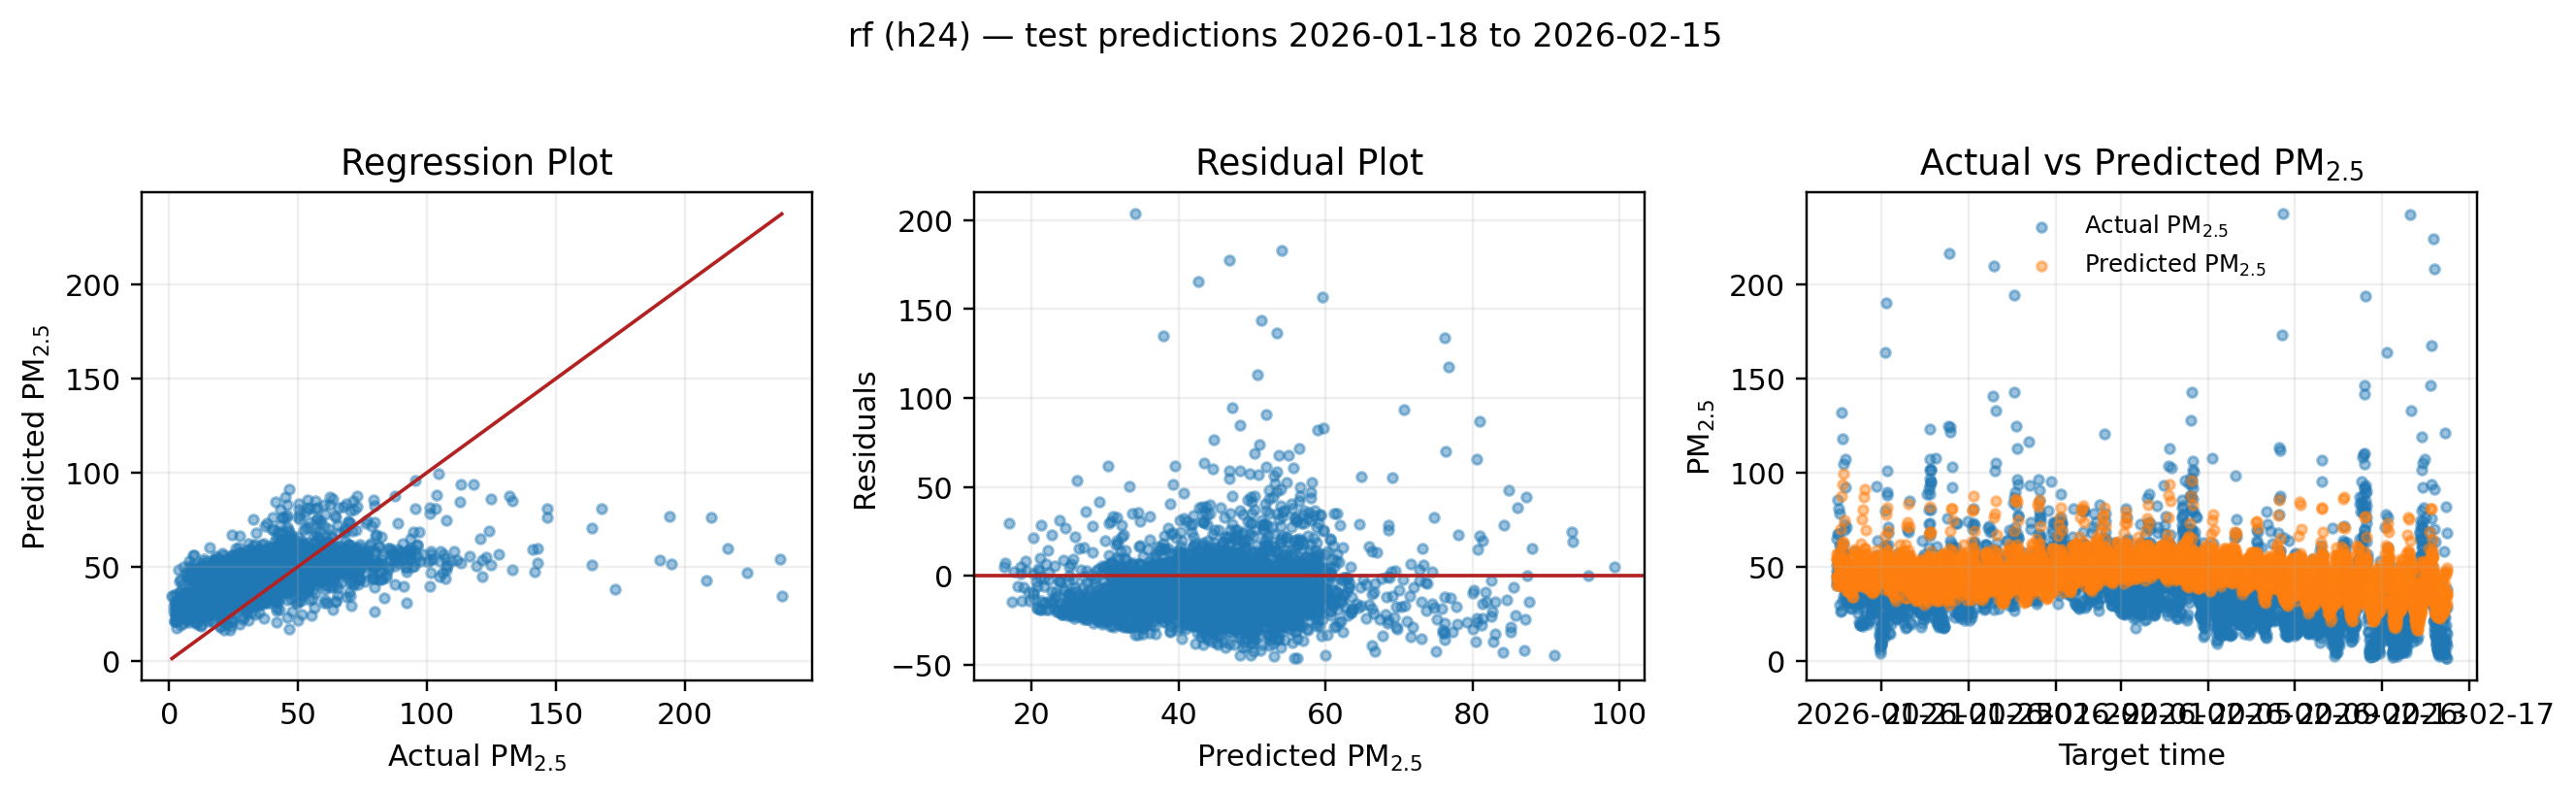
\includegraphics[width=0.85\textwidth]{figs/results_scatter_rf_h24.png}%
        \caption{Random Forest (tabular lags).}
    \end{subfigure}

    \begin{subfigure}[b]{\textwidth}
        \centering        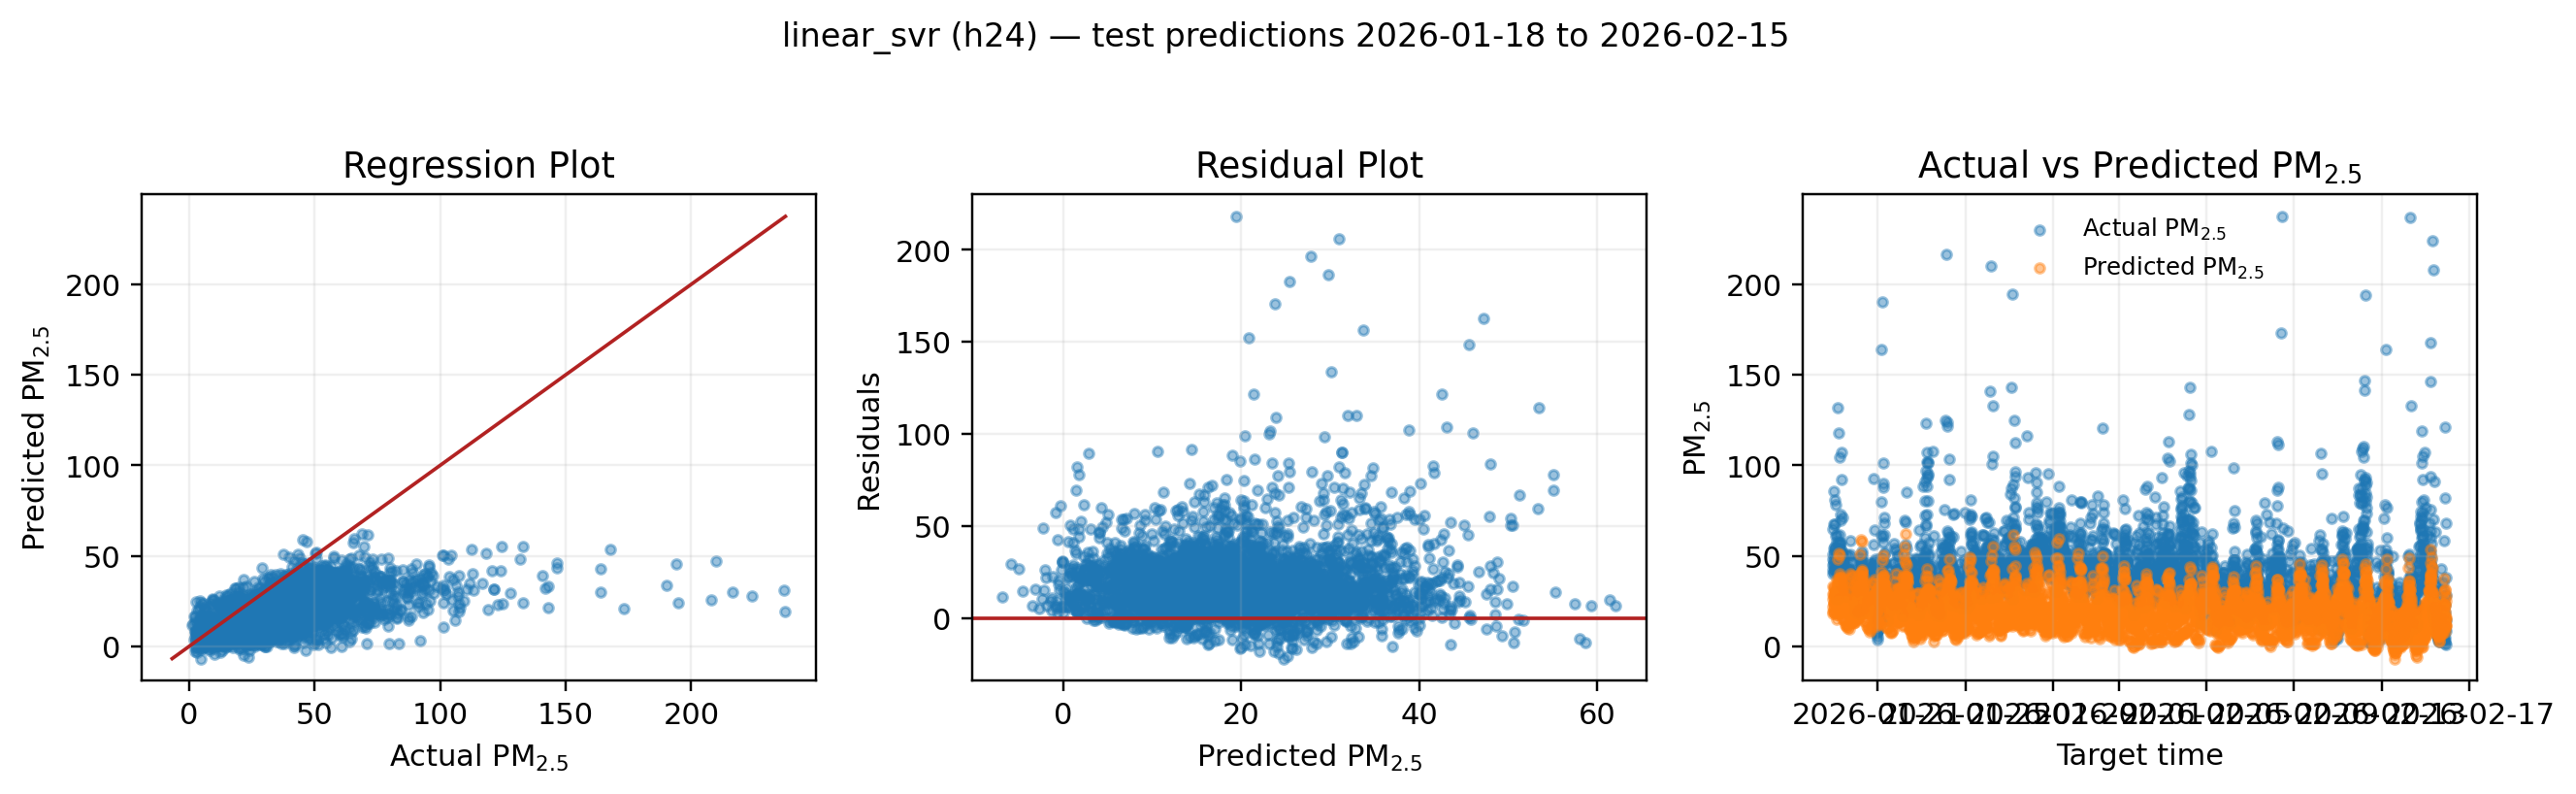
\includegraphics[width=0.95\textwidth]{figs/results_scatter_linear_svr_h24.png}%
        \caption{Linear SVR (tabular lags).}
    \end{subfigure}

    \begin{subfigure}[b]{\textwidth}
        \centering
        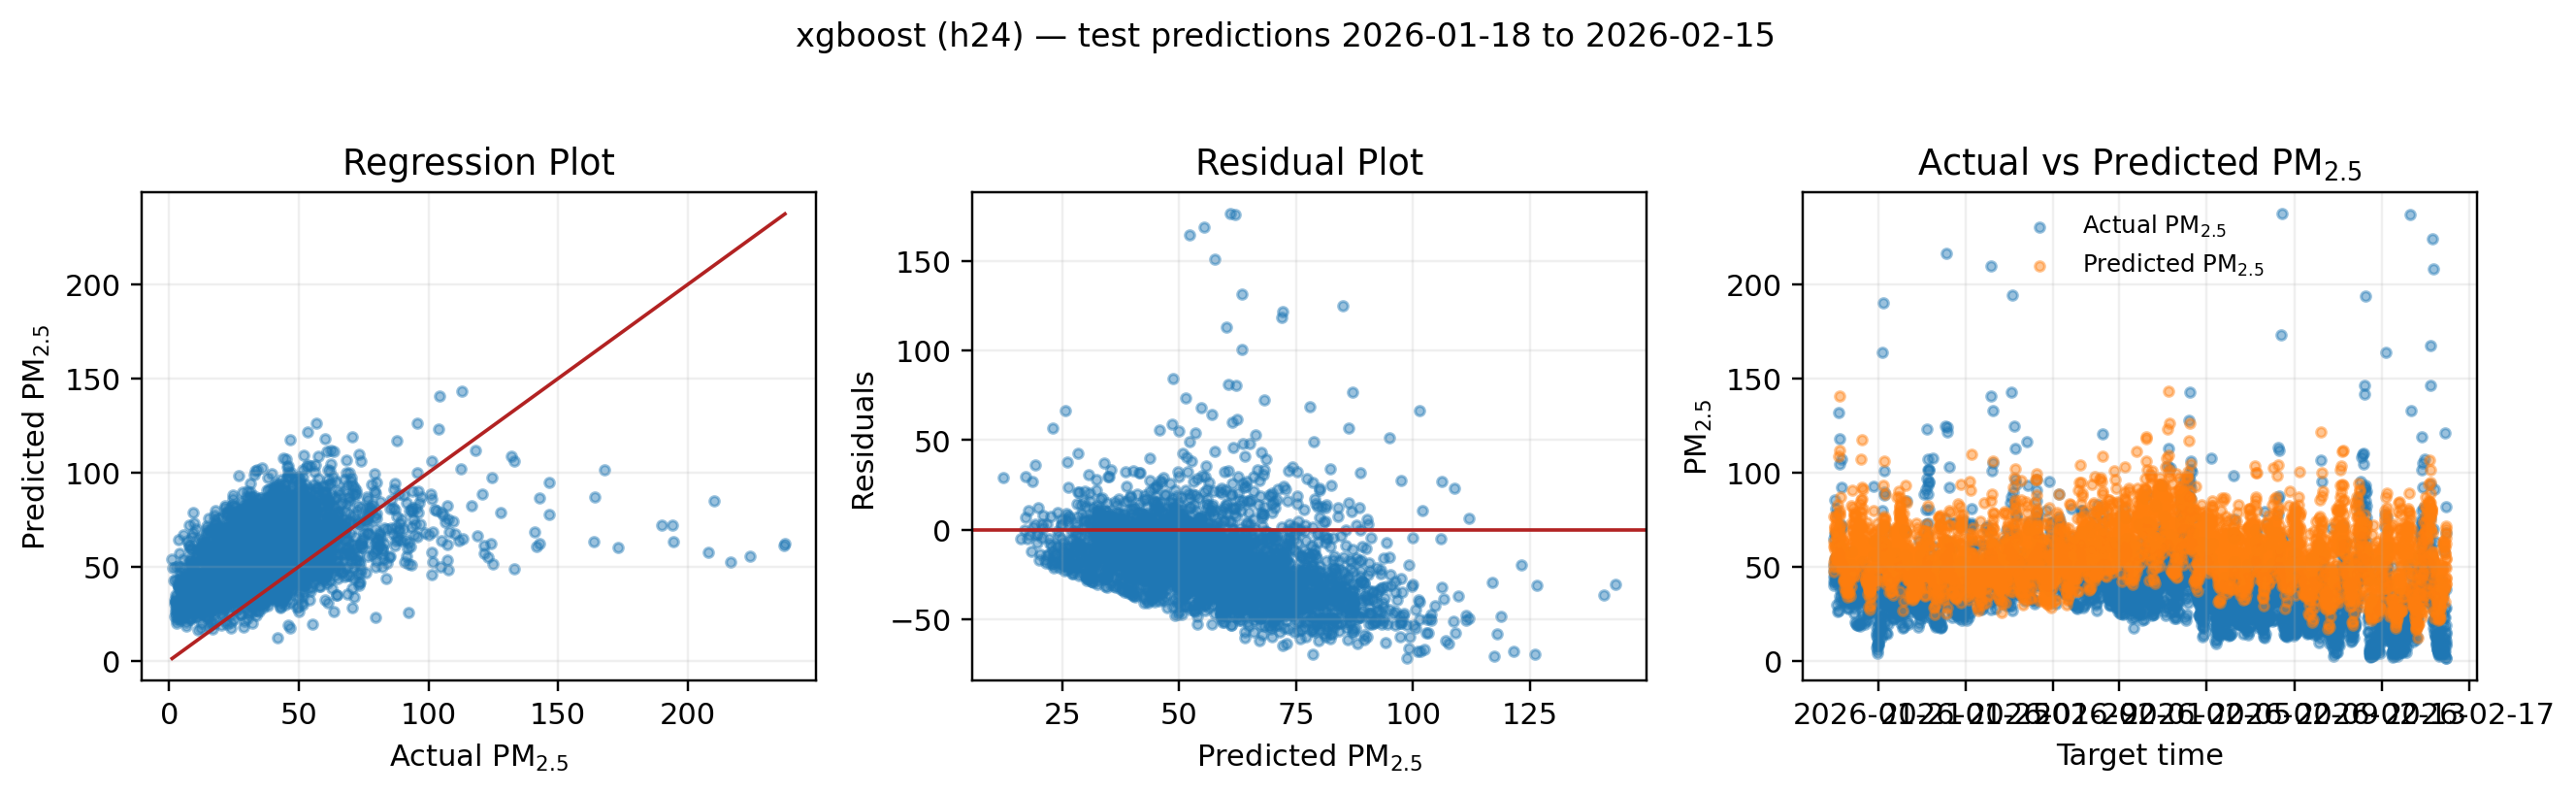
\includegraphics[width=0.95\textwidth]{figs/results_scatter_xgboost_h24.png}%
        \caption{XGBoost (tabular lags).}
    \end{subfigure}
    \caption{Diagnostic scatter plots for direct 24~h forecasts on the pooled multi-site test split, using exported test predictions (\texttt{reports/predictions/}; script~10). The layout mirrors standard regression and residual views: departure from the diagonal at high concentrations indicates conditional bias in the upper tail; the time overlay highlights how point forecasts track the bulk trajectory but often smooth short-lived spikes.}
    \label{fig:scatter_tabular_h24}
\end{figure}

Taken together, the pooled and upper-tail analyses show that good average forecasting performance did not translate directly into equivalent performance during high-pollution episodes.

\subsection{Diagnostic analyses}
\label{sec:diagnostics}

\prop{Two robustness checks were run after the headline scores were fixed. They do not replace Table~\ref{tab:forecast-summary}.}

\prop{A residual 24-h LSTM used the same architecture as the headline direct LSTM ($L=168$~h, 64 units, Adam $10^{-3}$, seed 42) but predicted $\Delta y=y_{t+24}-y_t$ and reconstructed $\hat{y}_{t+24}=y_t+\widehat{\Delta y}$ (Table~\ref{tab:lstm-h24-residual}). Test MAE was 12.68, below a same-run direct control (16.27) and the headline direct LSTM (23.19), near persistence (12.93) but still above Ridge (11.96).}
{\color{red}
\begin{table}[H]
\centering
\caption{24-h residual LSTM diagnostic on the same blocked split as Table~\ref{tab:forecast-summary}. Target $\Delta y=y_{t+24}-y_t$; reconstructed $\hat{y}_{t+24}=y_t+\widehat{\Delta y}$. Headline scores are not replaced.}
\label{tab:lstm-h24-residual}
\small
\begin{tabular}{lrr}
\toprule
Model & Val.\ MAE & Test MAE \\
\midrule
LSTM residual ($\Delta y+y_t$) & 10.92 & 12.68 \\
LSTM direct (same-run control) & 9.26 & 16.27 \\
Persistence ($y_t$) & 10.45 & 12.93 \\
Headline direct LSTM (Table~\ref{tab:forecast-summary}) & --- & 23.19 \\
Headline Ridge AR+Fourier & --- & 11.96 \\
\bottomrule
\end{tabular}
\end{table}
{\footnotesize\textit{Note.} $n_{\mathrm{train}}/n_{\mathrm{val}}/n_{\mathrm{test}}=14{,}379/1{,}016/3{,}807$. The same-run control uses the identical sequences, split and architecture as the residual model but was retrained independently (seed 42); its test MAE (16.27) differs from the headline direct LSTM (23.19, Table~\ref{tab:forecast-summary}) because of run-to-run variability in early stopping. The headline run used TensorFlow; this diagnostic used JAX.}
}

\prop{Because the 28-day attention increment over the joint LSTM without attention was not statistically supported, the attention forecast was mixed with the training-period mean of corrected PM$_{2.5}$ by hour-of-day and Harmattan regime (Table~\ref{tab:h28-clim-blend}): $\hat{y}=\alpha\hat{y}_{\mathrm{attn}}+(1-\alpha)\bar{y}_{\mathrm{clim}}$. Three fixed weights were evaluated without tuning. All three blends improved on attention alone and on the seasonal mean alone. This does not change the headline comparison among unblended model classes, and it does not change the paired attention-versus-joint-LSTM test, which remains non-significant.}
{\color{red}
\begin{table}[H]
\centering
\caption{28-day attention $\times$ climatology blend on the headline joint test rows ($n=1{,}957$). Weights $\alpha$ were pre-set and not tuned. Headline Table~\ref{tab:forecast-summary} is not replaced.}
\label{tab:h28-clim-blend}
\small
\begin{tabular}{lr}
\toprule
Model & 28-day Test MAE \\
\midrule
Attention only (\texttt{mh\_lstm\_mha}) & 13.56 \\
$\alpha=0.9$ & 12.89 \\
$\alpha=0.7$ & 11.99 \\
$\alpha=0.5$ & 11.91 \\
Seasonal mean only & 14.04 \\
\bottomrule
\end{tabular}
\end{table}
{\footnotesize\textit{Note.} Climatology is the training-period mean of corrected PM$_{2.5}$ by hour-of-day and Harmattan regime (local time before validation start). The 28-day test window is entirely Harmattan.}
}



% \subsection{Temporal diurnal variation in corrected PM$_{2.5}$ concentrations}

% Hourly PM$_{2.5}$ concentrations pooled across locations exhibited a pronounced diurnal cycle (Figure~\ref{fig:diurnal_pooled}). Mean concentrations increased during the early morning period and reached a maximum between 05:00 and 07:00, peaking at approximately 48 $\mu$g/m$^3$ around 06:00. Concentrations subsequently declined through midday, reaching minimum values between 13:00 and 14:00, before increasing again during evening hours. Median concentrations followed a similar temporal pattern.

% Diurnal profiles differed between Harmattan and pre-Harmattan periods (Figure~\ref{fig:diurnal_regime}). Under Harmattan conditions, median PM$_{2.5}$ concentrations remained elevated across all hours of the day. Midday median concentrations during Harmattan ranged between approximately 23–26 $\mu$g/m$^3$, compared with 8–12 $\mu$g/m$^3$ during pre-Harmattan periods. Early morning peaks were also higher during Harmattan, reaching approximately 50 $\mu$g/m$^3$ near 06:00, compared with approximately 36 $\mu$g/m$^3$ during pre-Harmattan conditions.
% \begin{figure}
%     \centering
%     \begin{subfigure}{0.48\textwidth}
%         \centering    \includegraphics[width=\linewidth]{figs/eda_diurnal_curve_pooled.png}%
%         \caption{Pooled hourly profile (mean, median, and interquartile band).}%
%         \label{fig:diurnal_pooled}
%     \end{subfigure}\hfill
%     \begin{subfigure}{0.48\textwidth}
%         \centering
%         \includegraphics[width=\linewidth]{figs/eda_diurnal_curve_by_regime.png}%
%         \caption{Median diurnal curves stratified by Harmattan versus pre-Harmattan conditions.}%
%         \label{fig:diurnal_regime}
%     \end{subfigure}
%     \caption{Diurnal variation in corrected PM$_{2.5}$ on local time (all sites pooled).}
%     \label{fig:diurnal}
% \end{figure}

% \subsection{Multi-horizon forecasting performance}

% Forecasting performance varied across models and prediction horizons (Table~\ref{tab:forecast-summary}; Figure~\ref{fig:forecast_mae}). At the 24 h horizon \rev{on the standard pooled test window}, Ridge AR+Fourier achieved the lowest MAE (11.96 $\mu$g/m$^3$; 95\% CI: 10.96–12.98), followed by the jointly trained multi-horizon LSTM (12.31 $\mu$g/m$^3$) and joint LSTM with attention (12.94 $\mu$g/m$^3$). \rev{Among gradient-boosted and ensemble tabular models, Random Forest recorded MAE 14.09 $\mu$g/m$^3$, Linear SVR 20.10 $\mu$g/m$^3$, and XGBoost 22.16 $\mu$g/m$^3$.} The per-horizon direct LSTM produced substantially higher error (23.19 $\mu$g/m$^3$) and a negative $R^2$ value ($R^2 = -1.344$). Seasonal naïve forecasting achieved an MAE of 13.76 $\mu$g/m$^3$.


% At the 7 d horizon, the jointly trained LSTM with attention (\texttt{mh\_lstm\_mha}) achieved the lowest pooled MAE of 11.32 $\mu$g/m$^3$ (95\% CI: 9.68–12.92). This outperformed the per-horizon LSTM (13.04 $\mu$g/m$^3$), joint LSTM without attention (15.02 $\mu$g/m$^3$), the weekly seasonal naïve baseline (15.39 $\mu$g/m$^3$)\rev{, and tabular models including Random Forest (19.08 $\mu$g/m$^3$), Linear SVR (37.21 $\mu$g/m$^3$), and XGBoost (43.46 $\mu$g/m$^3$)}. The attention-enhanced model also achieved an RMSE of 17.94 $\mu$g/m$^3$ and an $R^2$ of 0.155.

% At the 14 d horizon, the joint LSTM with attention recorded the strongest overall performance across experiments, achieving the lowest MAE (9.78 $\mu$g/m$^3$; 95\% CI: 8.69–10.80), RMSE (16.58 $\mu$g/m$^3$), and positive predictive performance ($R^2 = 0.108$). Alternative approaches, including per-horizon LSTM (14.31 $\mu$g/m$^3$), linear SVR (14.52 $\mu$g/m$^3$)\rev{, Ridge AR+Fourier (15.39 $\mu$g/m$^3$), Random Forest (19.64 $\mu$g/m$^3$), XGBoost (24.88 $\mu$g/m$^3$)}, and joint LSTM without attention (16.58 $\mu$g/m$^3$), recorded higher errors.



% At the 28 d horizon, forecasting accuracy decreased across models. Nevertheless, the joint LSTM with attention remained the best-performing model, achieving an MAE of 13.56 $\mu$g/m$^3$ (95\% CI: 11.25–16.35), compared with 14.92 $\mu$g/m$^3$ for joint LSTM without attention, 15.48 $\mu$g/m$^3$ for Ridge AR+Fourier\rev{, 15.62 $\mu$g/m$^3$ for Random Forest, 19.25 $\mu$g/m$^3$ for XGBoost, 23.48 $\mu$g/m$^3$ for Linear SVR}, and 17.99 $\mu$g/m$^3$ for the seasonal naïve benchmark. Predictive performance at this horizon was generally weaker, with low positive or negative $R^2$ values across models.

% \subsection{Regime-stratified forecasting performance across Harmattan and pre-Harmattan periods}

% Forecast accuracy differed between pre-Harmattan and Harmattan conditions on the extended 84-day regime-spanning test window (Tables \ref{tab:forecast-regime}–\ref{tab:tabular-regime-mae}). Simple benchmark models showed consistently higher prediction error during Harmattan than pre-Harmattan periods. At the 24 h horizon, the naïve persistence model recorded an overall MAE of 12.59 $\mu$g/m$^3$, increasing from 10.40 $\mu$g/m$^3$ during pre-Harmattan to 12.84 $\mu$g/m$^3$ during Harmattan. Similarly, the weekly seasonal naïve model increased from 10.86 $\mu$g/m$^3$ during pre-Harmattan to 14.10 $\mu$g/m$^3$ during Harmattan. Comparable patterns were observed at the 7 d horizon, where persistence and seasonal naïve models recorded Harmattan MAE values of 14.25 and 14.73 $\mu$g/m$^3$, respectively, compared with lower pre-Harmattan errors of 10.84 and 13.31 $\mu$g/m$^3$.
% % \begin{table}[H]
% % \centering
% % \caption{Forecast accuracy stratified by regime on a regime-spanning evaluation window (test window length increased to 84~days to include both pre-Harmattan and Harmattan periods). Values are MAE ($\mu$g/m$^3$) on the test set for simple benchmarks.}
% % \label{tab:forecast-regime}
% % \resizebox{0.95\textwidth}{!}{%
% % \begin{tabular}{llrrr}
% % \toprule
% % Horizon & Model & Overall MAE & Pre-Harmattan MAE & Harmattan MAE \\
% % \midrule
% % 24~h & Naïve level (persistence) & 12.59 & 10.40 & 12.84 \\
% % 24~h & Seasonal naïve (weekly anchor) & 13.75 & 10.86 & 14.10 \\
% % \midrule
% % 7~d (168~h) & Naïve level (persistence) & 13.61 & 10.84 & 14.25 \\
% % 7~d (168~h) & Seasonal naïve (weekly anchor) & 14.46 & 13.31 & 14.73 \\
% % \bottomrule
% % \end{tabular}}
% % \end{table}

% Among tabular forecasting models, Random Forest consistently achieved the lowest MAE across most horizons on the extended regime-aware test window (Table \ref{tab:tabular-regime-mae}). At 24 h, Random Forest achieved an overall MAE of 10.33 $\mu$g/m$^3$, outperforming Ridge AR+Fourier (16.79 $\mu$g/m$^3$), Linear SVR (14.61 $\mu$g/m$^3$), and XGBoost (10.90 $\mu$g/m$^3$). Random Forest also recorded the lowest pre-Harmattan and Harmattan MAE values at this horizon (7.89 and 10.61 $\mu$g/m$^3$, respectively). Similar performance patterns were observed at 7 d and 14 d, where Random Forest achieved overall MAE values of 12.01 and 11.73 $\mu$g/m$^3$, respectively, compared with substantially higher errors for Ridge AR+Fourier and Linear SVR.
% \begin{table}[H]
% \centering
% \caption{Tabular models: test-set MAE ($\mu$g/m$^3$) stratified by Harmattan regime on an \textbf{84-day} label-time held-out window (both regimes present)}
% \label{tab:tabular-regime-mae}
% \resizebox{0.70\textwidth}{!}{%
% \begin{tabular}{llrrr}
% \toprule
% Horizon & Model & Overall MAE & Pre-Harmattan MAE & Harmattan MAE \\
% \midrule
% 24~h & Ridge AR+Fourier & 16.79 & 10.55 & 17.51 \\
% 24~h & Random Forest (tabular lags) & 10.33 & 7.89 & 10.61 \\
% 24~h & Linear SVR (tabular lags) & 14.61 & 9.77 & 15.17 \\
% 24~h & XGBoost (tabular lags) & 10.90 & 8.81 & 11.15 \\
% \midrule
% 7~d (168~h) & Ridge AR+Fourier & 35.25 & 12.19 & 40.40 \\
% 7~d (168~h) & Random Forest (tabular lags) & 12.01 & 8.56 & 12.78 \\
% 7~d (168~h) & Linear SVR (tabular lags) & 13.58 & 8.86 & 14.63 \\
% 7~d (168~h) & XGBoost (tabular lags) & 12.89 & 9.76 & 13.59 \\
% \midrule
% 14~d (336~h) & Ridge AR+Fourier & 48.80 & 34.82 & 54.06 \\
% 14~d (336~h) & Random Forest (tabular lags) & 11.73 & 9.85 & 12.44 \\
% 14~d (336~h) & Linear SVR (tabular lags) & 33.74 & 21.33 & 38.41 \\
% 14~d (336~h) & XGBoost (tabular lags) & 13.38 & 11.51 & 14.09 \\
% \midrule
% 28~d (672~h) & Ridge AR+Fourier & 63.08 & 27.13 & 93.17 \\
% 28~d (672~h) & Random Forest (tabular lags) & 13.04 & 10.86 & 14.87 \\
% 28~d (672~h) & Linear SVR (tabular lags) & 41.02 & 17.32 & 60.86 \\
% 28~d (672~h) & XGBoost (tabular lags) & 14.44 & 12.25 & 16.27 \\
% \bottomrule
% \end{tabular}}
% \end{table}

% Forecast degradation during Harmattan became increasingly pronounced at longer horizons. Ridge AR+Fourier showed marked increases in prediction error during Harmattan, rising from 12.19 $\mu$g/m$^3$ during pre-Harmattan to 40.40 $\mu$g/m$^3$ at 7 d, from 34.82 to 54.06 $\mu$g/m$^3$ at 14 d, and from 27.13 to 93.17 $\mu$g/m$^3$ at 28 d. Linear SVR exhibited similar deterioration, with Harmattan MAE increasing to 60.86 $\mu$g/m$^3$ at 28 d. In contrast, Random Forest and XGBoost maintained comparatively stable performance across regimes and horizons. At 28 d, Random Forest achieved an overall MAE of 13.04 $\mu$g/m$^3$ and Harmattan MAE of 14.87 $\mu$g/m$^3$, while XGBoost recorded 14.44 and 16.27 $\mu$g/m$^3$, respectively.

% \subsection{Performance during high-pollution episodes}

% Forecasting errors increased substantially during upper-decile pollution periods (Table \ref{tab:forecast-upper-decile}). At the 24 h horizon, MAE$^{90}$ ranged from 28.95 $\mu$g/m$^3$ for the joint LSTM with attention to 53.36 $\mu$g/m$^3$ for the per-horizon LSTM, compared with pooled MAE values of 11.96–23.19 $\mu$g/m$^3$. Similar patterns were observed at longer horizons. At 7 d, the joint LSTM with attention achieved a pooled MAE of 11.32 $\mu$g/m$^3$, whereas MAE$^{90}$ increased to 33.45 $\mu$g/m$^3$. At 14 d, MAE$^{90}$ for the same model reached 33.35 $\mu$g/m$^3$, despite a pooled MAE of 9.78 $\mu$g/m$^3$. At 28 d, MAE$^{90}$ remained elevated at 32.17 $\mu$g/m$^3$.
% \begin{table}[H]
% \centering
% \caption{Pooled MAE versus upper-decile MAE (MAE$^{90}$: mean absolute error on test hours whose observed PM$_{2.5}$ is at or above the 90th percentile of observed concentrations in the test window). Sequence rows are from deep-model metrics; tabular rows are from tabular-model metrics.}
% \label{tab:forecast-upper-decile}
% \resizebox{0.70\textwidth}{!}{%
% \begin{tabular}{llrr}
% \toprule
% Horizon & Model & MAE & MAE$^{90}$ \\
% \midrule
% 24~h & Ridge AR+Fourier & 11.96 & 35.65 \\
% 24~h & Joint multi-horizon LSTM (\texttt{mh\_lstm}) & 12.31 & 39.61 \\
% 24~h & Joint multi-horizon LSTM + attention (\texttt{mh\_lstm\_mha}) & 12.94 & 28.95 \\
% 24~h & Random Forest (tabular lags) & 14.09 & 27.04 \\
% 24~h & Linear SVR (tabular lags) & 20.10 & 51.93 \\
% 24~h & XGBoost (tabular lags) & 22.16 & 22.90 \\
% 24~h & LSTM (per-horizon direct) & 23.19 & 53.36 \\
% \midrule
% 7~d (168~h) & Joint multi-horizon LSTM + attention (\texttt{mh\_lstm\_mha}) & 11.32 & 33.45 \\
% 7~d (168~h) & Random Forest (tabular lags) & 19.08 & 22.93 \\
% 7~d (168~h) & Linear SVR (tabular lags) & 37.21 & 69.48 \\
% 7~d (168~h) & XGBoost (tabular lags) & 43.46 & 28.81 \\
% 7~d (168~h) & LSTM (per-horizon direct) & 13.04 & 33.97 \\
% 7~d (168~h) & Joint multi-horizon LSTM (\texttt{mh\_lstm}) & 15.02 & 42.42 \\
% \midrule
% 14~d (336~h) & Joint multi-horizon LSTM + attention (\texttt{mh\_lstm\_mha}) & 9.78 & 33.35 \\
% 14~d (336~h) & Linear SVR (tabular lags) & 14.52 & 26.53 \\
% 14~d (336~h) & LSTM (per-horizon direct) & 14.31 & 43.51 \\
% 14~d (336~h) & Random Forest (tabular lags) & 19.64 & 24.15 \\
% 14~d (336~h) & XGBoost (tabular lags) & 24.88 & 20.43 \\
% 14~d (336~h) & Joint multi-horizon LSTM (\texttt{mh\_lstm}) & 16.58 & 40.84 \\
% \midrule
% 28~d (672~h) & Joint multi-horizon LSTM + attention (\texttt{mh\_lstm\_mha}) & 13.56 & 32.17 \\
% 28~d (672~h) & Joint multi-horizon LSTM (\texttt{mh\_lstm}) & 14.92 & 39.61 \\
% 28~d (672~h) & Ridge AR+Fourier & 15.48 & 32.73 \\
% 28~d (672~h) & Random Forest (tabular lags) & 15.62 & 27.80 \\
% 28~d (672~h) & XGBoost (tabular lags) & 19.25 & 26.66 \\
% 28~d (672~h) & Linear SVR (tabular lags) & 23.48 & 26.50 \\
% \bottomrule
% \end{tabular}}
% \end{table}

% Figure \ref{fig:scatter_tabular_h24} presents point-level diagnostics for direct 24 h forecasts generated using Random Forest, Linear SVR, and XGBoost models. Scatter plots of observed versus predicted PM${2.5}$ concentrations showed clustering around the $y=x$ reference line at low-to-moderate concentrations across all models, indicating reasonable predictive agreement in the central range of observations. However, deviations from the reference line increased at higher PM${2.5}$ concentrations, indicating reduced predictive accuracy during elevated pollution conditions.
% % \begin{figure}[H]
% %     \centering
% %     \begin{subfigure}[b]{\textwidth}
% %         \centering
% %         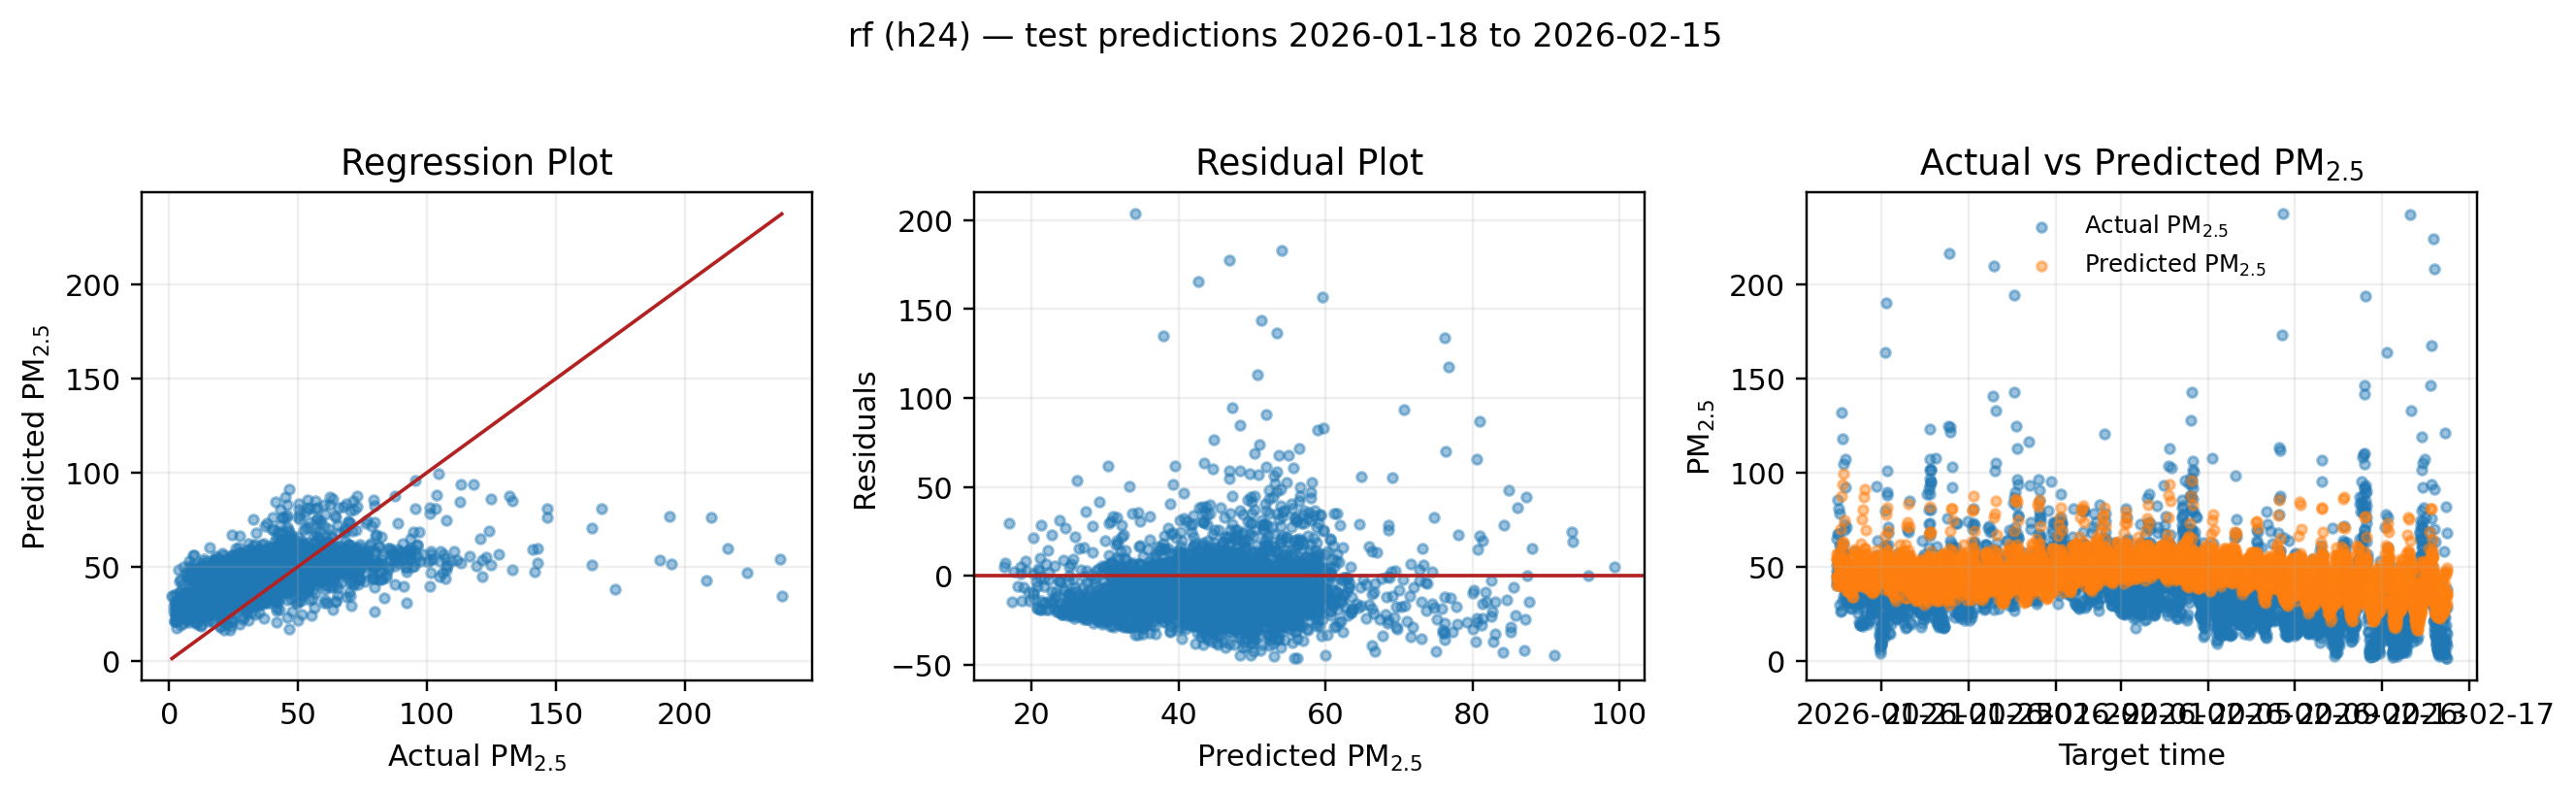
\includegraphics[width=0.85\textwidth]{figs/results_scatter_rf_h24.png}%
% %         \caption{Random Forest (tabular lags).}
% %     \end{subfigure}

% %     \begin{subfigure}[b]{\textwidth}
% %         \centering        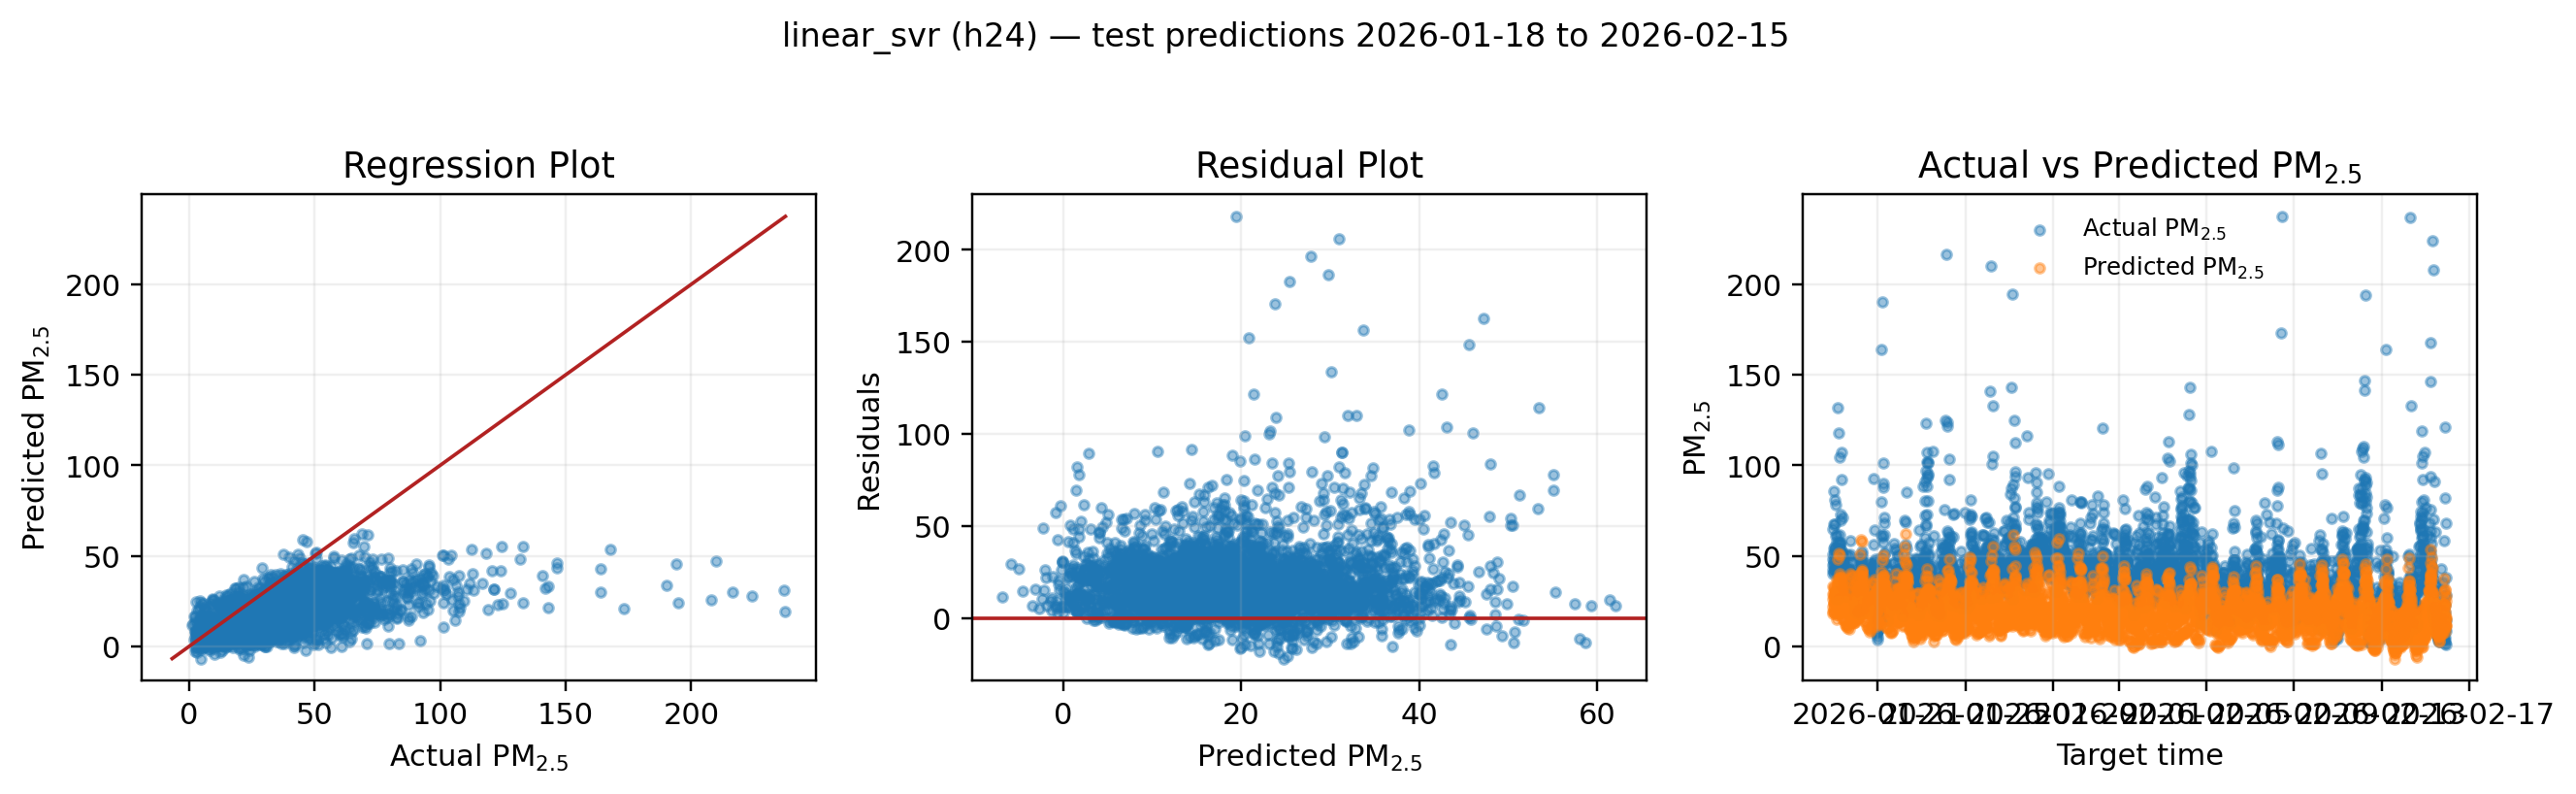
\includegraphics[width=0.95\textwidth]{figs/results_scatter_linear_svr_h24.png}%
% %         \caption{Linear SVR (tabular lags).}
% %     \end{subfigure}

% %     \begin{subfigure}[b]{\textwidth}
% %         \centering
% %         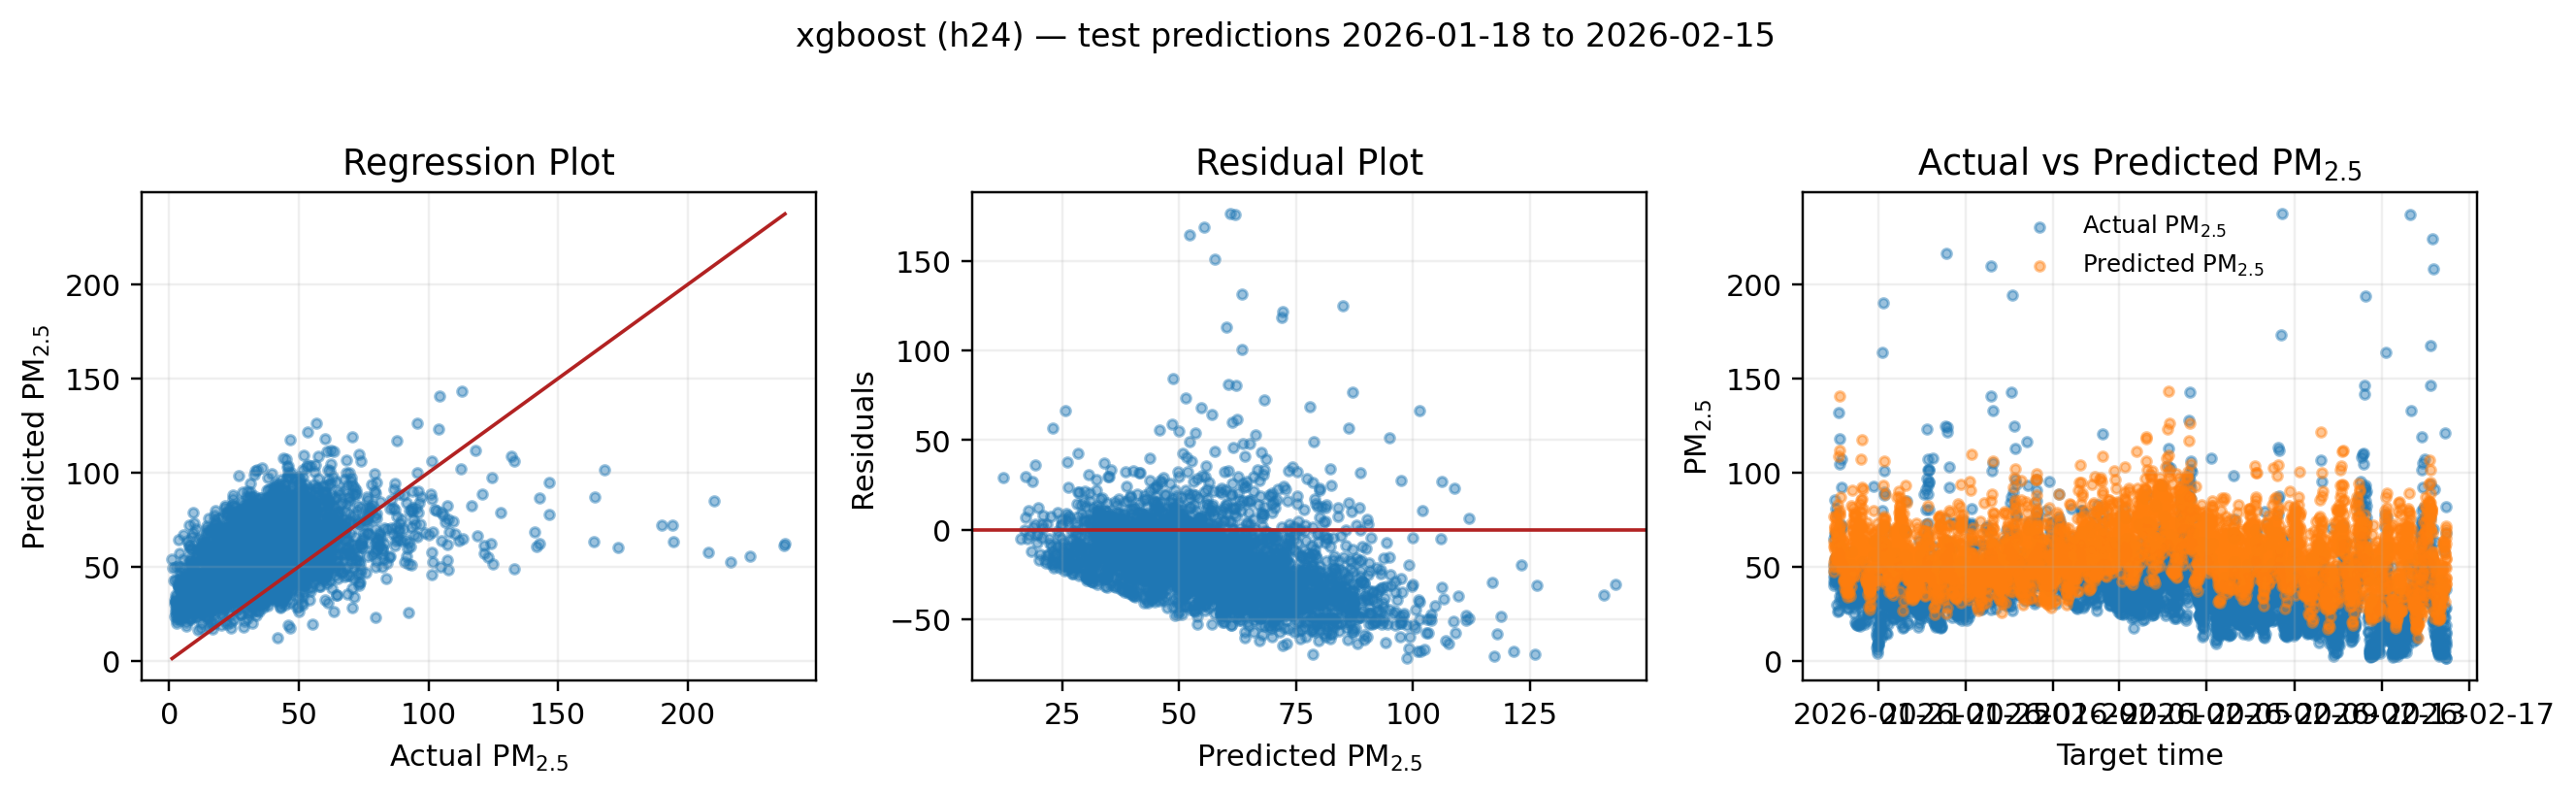
\includegraphics[width=0.95\textwidth]{figs/results_scatter_xgboost_h24.png}%
% %         \caption{XGBoost (tabular lags).}
% %     \end{subfigure}
% %     \caption{Diagnostic scatter plots for direct 24~h forecasts on the pooled multi-site test split, using exported test predictions (\texttt{reports/predictions/}; script~10). The layout mirrors standard regression and residual views: departure from the diagonal at high concentrations indicates conditional bias in the upper tail; the time overlay highlights how point forecasts track the bulk trajectory but often smooth short-lived spikes.}
% %     \label{fig:scatter_tabular_h24}
% % \end{figure}

% Residual plots revealed increasing error dispersion at higher predicted concentrations, particularly for Linear SVR, whereas Random Forest and XGBoost exhibited comparatively narrower residual spread. Time-series overlays further showed that all three models broadly tracked temporal trends in PM$_{2.5}$ during the held-out test period. Nonetheless, short-duration, high-concentration episodes appeared smoother in the predicted series than in the observed values, particularly during abrupt pollution spikes. Random Forest and XGBoost visually demonstrated closer alignment with observed trajectories than Linear SVR across the test window.


% \subsection{Statistical comparison of competing models}

% Paired significance testing (Table \ref{tab:significance}) indicated no statistically significant advantage of joint attention over joint LSTM at the 24 h horizon. However, at 7 d and 14 d, the joint LSTM with attention significantly reduced prediction error relative to the joint LSTM model, with approximate $\Delta$MAE reductions of 3.7 and 6.8 $\mu$g/m$^3$, respectively. At 28 d, the joint attention model significantly outperformed Ridge AR+Fourier, although no significant difference was observed relative to joint LSTM. \rev{Joint attention also significantly outperformed Random Forest, Linear SVR (except at 24~h), and XGBoost at most horizons on row-aligned test predictions.}



% \subsection{Distribution of corrected PM$_{2.5}$ Concentrations in locations}
% Corrected PM$_{2.5}$ concentrations are markedly heterogeneous across the seven fixed monitoring locations in Tema. Summary statistics in Table~\ref{tab:timeseries-data} show site-level means of approximately \mbox{19--35~$\mu$g/m$^3$}, with the highest central tendency at Divine Healer's Church (mean 35.15~$\mu$g/m$^3$; median 33.4~$\mu$g/m$^3$) and comparatively lower levels at Tema Community~25 Estate (mean 19.12~$\mu$g/m$^3$; median 16.1~$\mu$g/m$^3$). Interquartile ranges differ by site (roughly 15--28~$\mu$g/m$^3$), indicating that variability---not only average exposure---depends on micro-environment. Positive skewness in PM$_{2.5}$ is present at every site (skewness from about 1.1 to 3.2), consistent with episodic excursions rather than tightly symmetric fluctuations.

% Figure~\ref{fig:pm25_distribution} visualises these contrasts using raw and corrected distributions by location. The figure highlights wider dispersion and heavier upper tails at sites such as Divine Healer's Church and Satet International School, reinforcing that pollution risk is spatially structured and repeatedly punctuated by high-concentration episodes across the monitoring network.

% \begin{figure*}[t]
%     \centering
%     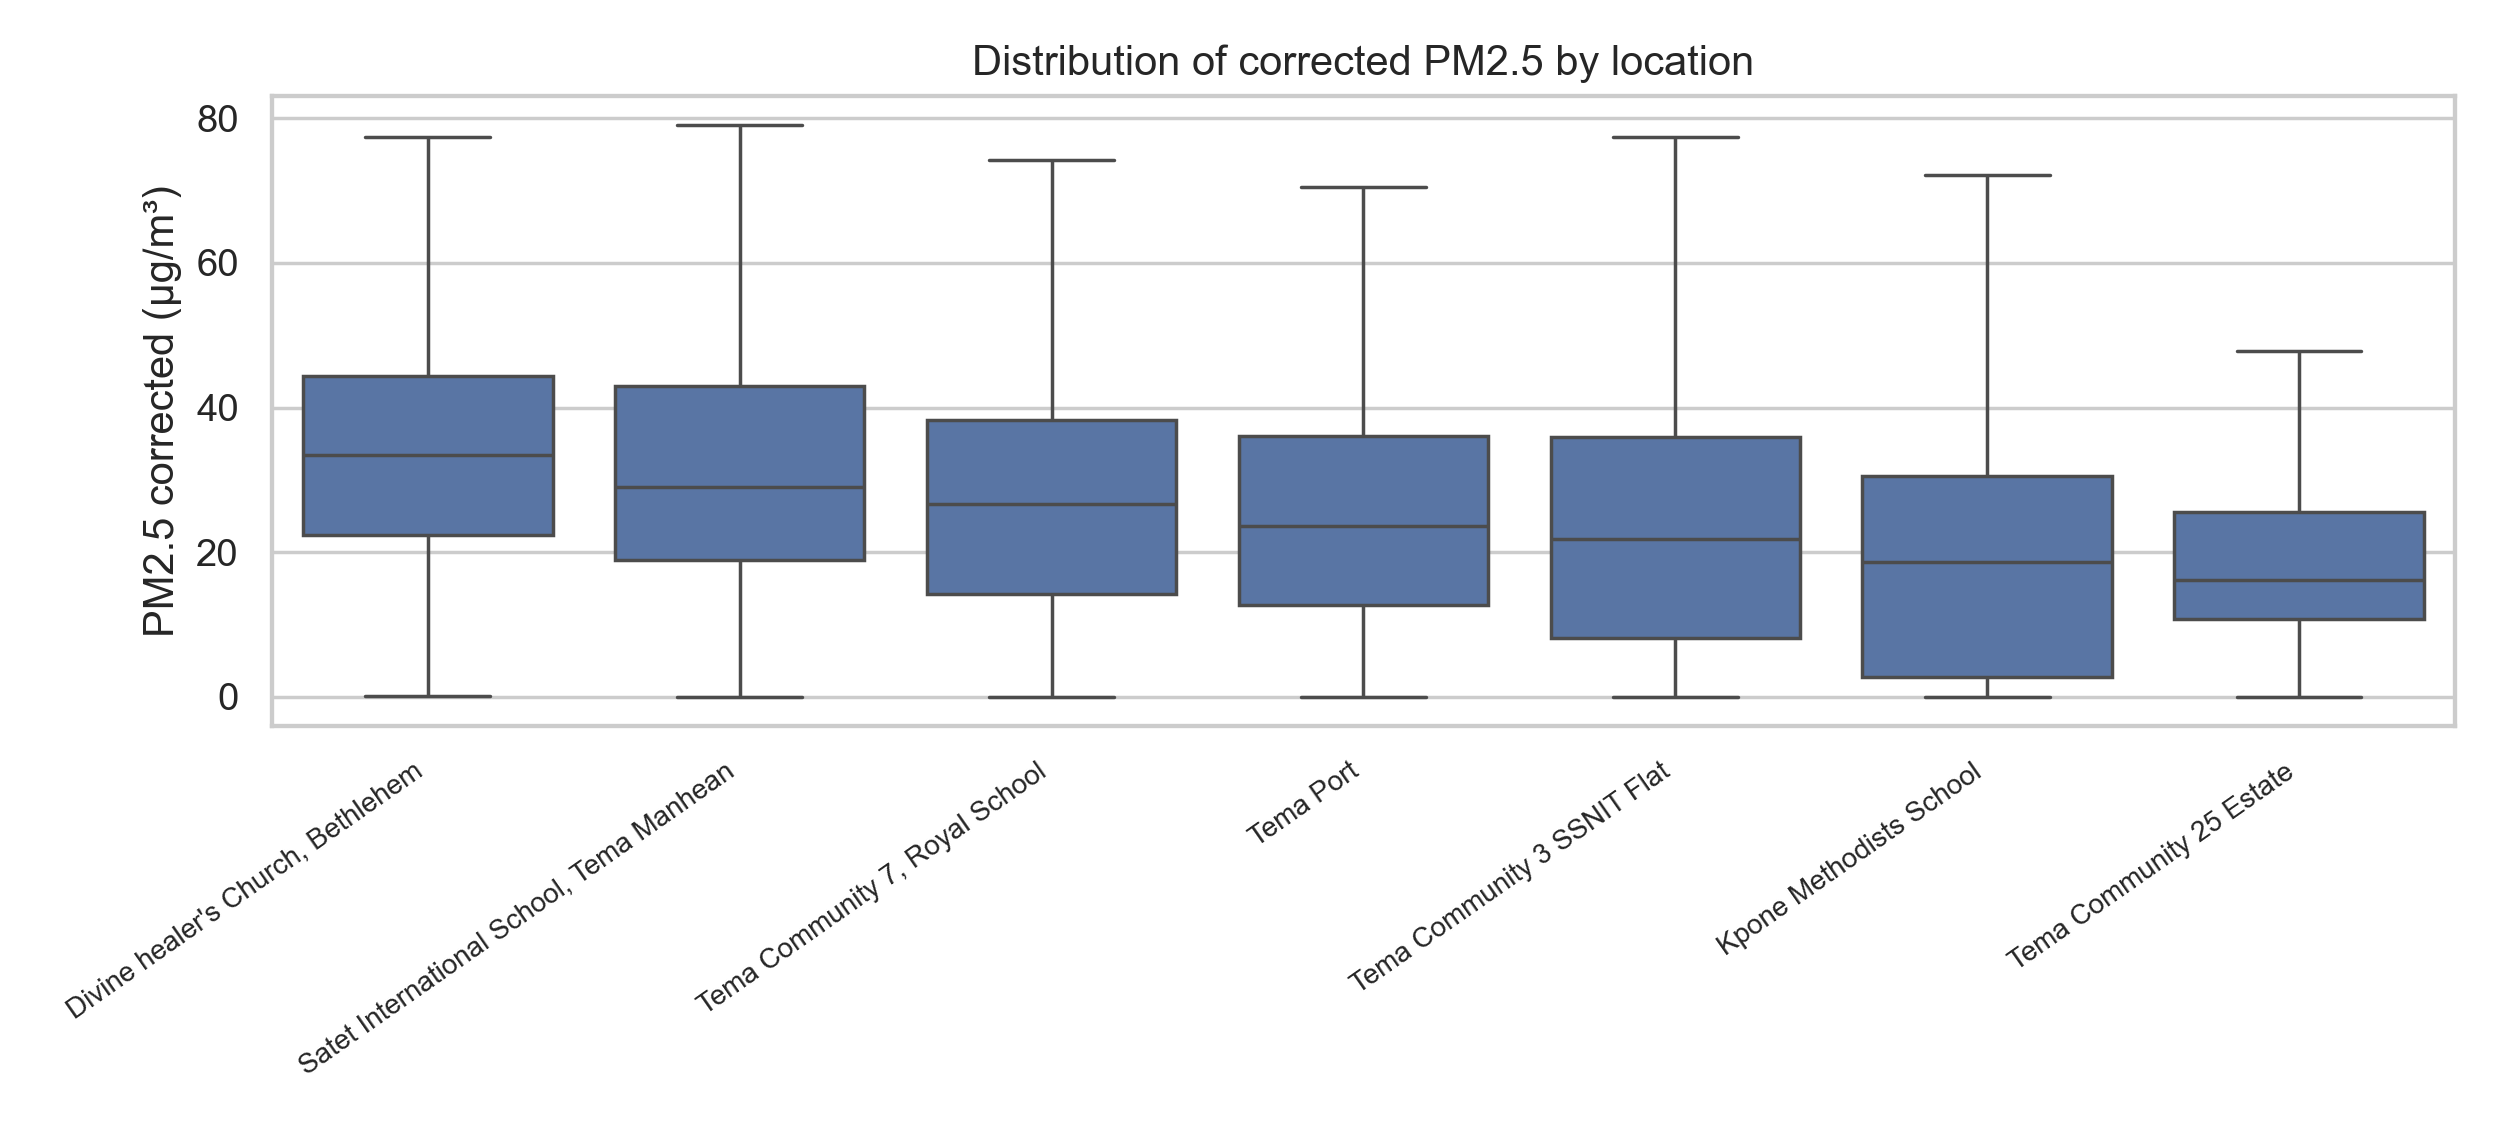
\includegraphics[width=0.92\textwidth]{figs/eda_pm25_boxplot_by_location.png}%
%     \caption{Distribution of raw and corrected PM$_{2.5}$ ($\mu$g/m$^3$) by monitoring location.}
%     \label{fig:pm25_distribution}
% \end{figure*}

% \subsection{Temporal diurnal Variation in corrected PM$_{2.5}$ Concentrations}
% Pooling all locations on local hourly time, corrected PM$_{2.5}$ exhibits a pronounced diurnal cycle (Figure~\ref{fig:diurnal_pooled}). Pooled hourly means rise toward a morning maximum around 05:00--07:00 (means up to approximately 48~$\mu$g/m$^3$ near 06:00), decline through midday, and reach an afternoon minimum around 13:00--14:00 (median near 15--17~$\mu$g/m$^3$), before increasing again through evening hours. This profile is broadly consistent with coupled influences of boundary-layer ventilation, emission activity rhythms, and regional aerosol transport.

% Harmattan versus pre-Harmattan regimes further reshape the diurnal curve (Figure~\ref{fig:diurnal_regime}). Under Harmattan conditions, pooled median concentrations remain elevated throughout the day; for example, median PM$_{2.5}$ near midday is substantially higher than under pre-Harmattan conditions at comparable clock hours (Harmattan midday medians near 23--26~$\mu$g/m$^3$ versus about 8--12~$\mu$g/m$^3$ pre-Harmattan). Early-morning peaks are likewise amplified during Harmattan (median near 50~$\mu$g/m$^3$ around 06:00) compared with pre-Harmattan (median near 36~$\mu$g/m$^3$). Together, Figures~\ref{fig:diurnal_pooled}--\ref{fig:diurnal_regime} motivate reporting forecast performance under pooled conditions while interpreting limitations whenever models must generalize across sharply different atmospheric regimes.

% \begin{figure*}[t]
%     \centering
%     \begin{subfigure}[t]{0.48\textwidth}
%         \centering
%         \includegraphics[width=\linewidth]{figs/eda_diurnal_curve_pooled.png}%
%         \caption{Pooled hourly profile (mean, median, and interquartile band).}%
%         \label{fig:diurnal_pooled}
%     \end{subfigure}\hfill
%     \begin{subfigure}[t]{0.48\textwidth}
%         \centering
%         \includegraphics[width=\linewidth]{figs/eda_diurnal_curve_by_regime.png}%
%         \caption{Median diurnal curves stratified by Harmattan versus pre-Harmattan conditions.}%
%         \label{fig:diurnal_regime}
%     \end{subfigure}
%     \caption{Diurnal variation in corrected PM$_{2.5}$ on local time (all sites pooled).}
%     \label{fig:diurnal}
% \end{figure*}

% \subsection{Temporal Multi-Horizon predictions}
% Forecasting models are trained and evaluated as \emph{direct} horizon-specific regressors on leakage-safe splits defined by label time (Section~\ref{sec2}), with horizons $H\in\{24,168,336,672\}$ hours. Table~\ref{tab:eval-splits} reports train, validation, and test row counts and the test-window start date for each horizon (label-time contiguous blocks; the most recent segment is held out for testing). Pooled metrics, bootstrap 95\% CIs, paired significance tests (Table~\ref{tab:significance}), upper-decile MAE, and the figures below are generated from exported test predictions and merged pipeline outputs (scripts~05/07 $\rightarrow$ 12 $\rightarrow$ 08 $\rightarrow$ 13; figures via scripts~09--10, 15).

% Figure~\ref{fig:forecast_mae} summarises pooled test-set MAE across horizons for a compact set of interpretable benchmarks, with 95\% bootstrap confidence intervals where available. In addition to per-horizon sequence models (LSTM and LSTM with multi-head attention), we include jointly trained multi-horizon sequence models (``mh\_lstm'' and ``mh\_lstm\_mha'') to test whether sharing information across lead times improves generalisation. The chart highlights that joint LSTM+attention attains the lowest pooled MAE at 7--28~days among sequence models in this window, while the upper tail remains challenging for all approaches (Table~\ref{tab:forecast-upper-decile}).

% \begin{figure*}[t]
%     \centering
%     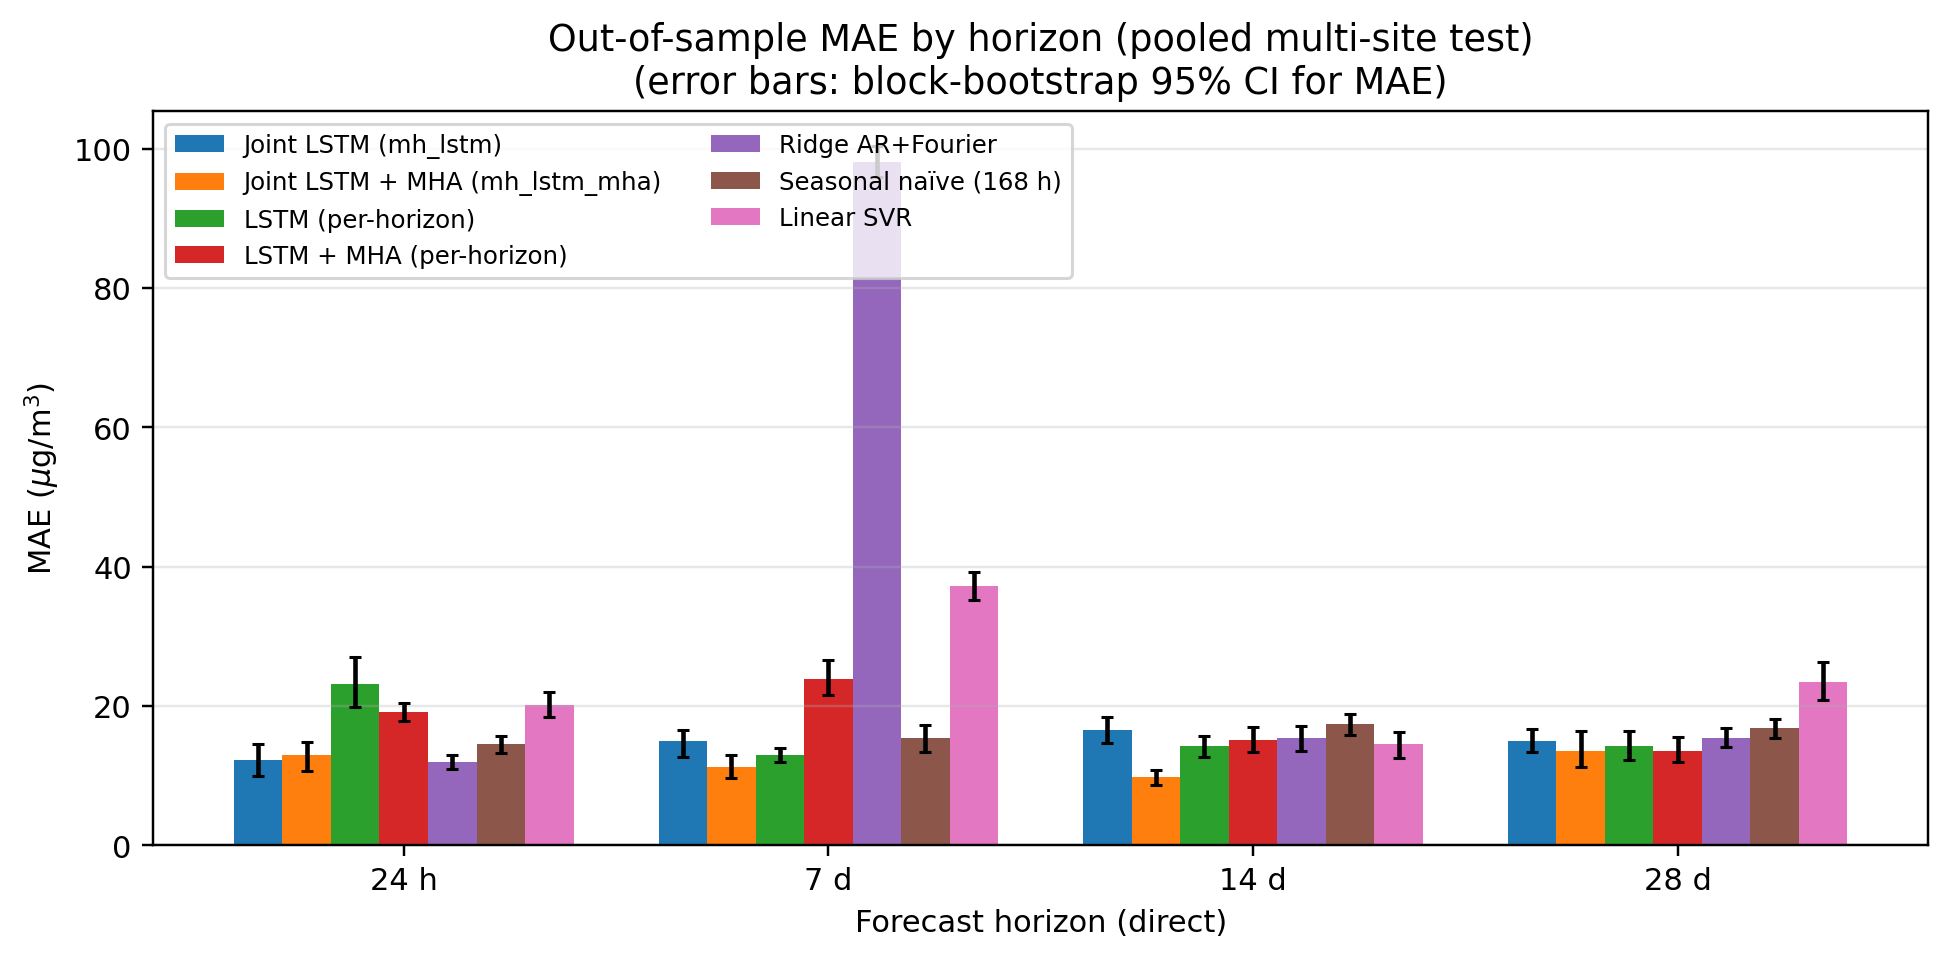
\includegraphics[width=0.92\textwidth]{figs/results_mae_by_horizon.png}%
%     \caption{Mean absolute error (MAE; $\mu$g/m$^3$) on pooled multi-site test windows for selected models, shown by direct forecasting horizon. Error bars denote 95\% percentile intervals from a moving-block bootstrap ($B{=}1000$, block length 168~h) on time-ordered test rows.}
%     \label{fig:forecast_mae}
% \end{figure*}

% Table~\ref{tab:forecast-summary} complements Figure~\ref{fig:forecast_mae} with RMSE and $R^2$ alongside pooled MAE and block-bootstrap 95\% CIs for headline models. Table~\ref{tab:significance} reports pre-specified paired $\Delta$MAE tests on aligned rows. Episode-focused error on hours whose realised PM$_{2.5}$ lies in the upper decile of the test window (MAE$^{90}$) is reported in Table~\ref{tab:forecast-upper-decile}; values there are typically far larger than pooled MAE, reflecting the heavy upper tail documented in Section~3.1. Systematic feature-importance or ablation analysis is \emph{not} included in this version (see Limitations).

% \begin{table}[H]
% \centering
% \caption{Evaluation splits by direct-forecast horizon (label-time contiguous blocks). $n$ counts hourly forecast rows after feature construction; test rows are the held-out tail of the study period.}
% \label{tab:eval-splits}
% \resizebox{0.60\textwidth}{!}{%
% \begin{tabular}{lrrrr}
% \toprule
% Horizon & $n_{\mathrm{train}}$ & $n_{\mathrm{val}}$ & $n_{\mathrm{test}}$ & Test window starts (local) \\
% \midrule
% 24~h & 17\,285 & 1\,827 & 4\,037 & 2026-01-18 \\
% 7~d (168~h) & 16\,277 & 1\,827 & 4\,037 & 2026-01-18 \\
% 14~d (336~h) & 15\,101 & 1\,827 & 4\,037 & 2026-01-18 \\
% 28~d (672~h) & 13\,263 & 1\,827 & 4\,037 & 2026-01-18 \\
% \bottomrule
% \end{tabular}}
% \end{table}

% \begin{table}[H]
% \centering
% \caption{Representative out-of-sample forecasting accuracy on pooled multi-site test splits (corrected PM$_{2.5}$, $\mu$g/m$^3$). ``mh\_lstm'' / ``mh\_lstm\_mha'' are jointly trained multi-horizon sequence models. MAE 95\% CI: moving-block bootstrap on exported test predictions ($B{=}1000$, block length 168~h).}
% \label{tab:forecast-summary}
% \resizebox{\textwidth}{!}{%
% \begin{tabular}{llrrrr}
% \toprule
% Horizon & Model & MAE & MAE 95\% CI & RMSE & $R^2$ \\
% \midrule
% 24~h & Ridge AR+Fourier & 11.96 & [10.96, 12.98] & 18.22 & 0.210 \\
% 24~h & Joint multi-horizon LSTM (\texttt{mh\_lstm}) & 12.31 & [9.99, 14.59] & 19.23 & 0.028 \\
% 24~h & Joint multi-horizon LSTM + attention (\texttt{mh\_lstm\_mha}) & 12.94 & [10.66, 14.87] & 18.30 & 0.120 \\
% 24~h & LSTM (per-horizon direct) & 23.19 & [19.92, 27.08] & 30.24 & $-1.344$ \\
% 24~h & Seasonal naïve (24h anchor) & 13.76 & [12.24, 15.10] & 21.94 & $-0.144$ \\
% \midrule
% 7~d (168~h) & Joint multi-horizon LSTM + attention (\texttt{mh\_lstm\_mha}) & 11.32 & [9.68, 12.92] & 17.94 & 0.155 \\
% 7~d (168~h) & LSTM (per-horizon direct) & 13.04 & [11.92, 14.05] & 18.80 & 0.207 \\
% 7~d (168~h) & Joint multi-horizon LSTM (\texttt{mh\_lstm}) & 15.02 & [12.75, 16.59] & 21.55 & $-0.219$ \\
% 7~d (168~h) & Seasonal naïve (weekly anchor) & 15.39 & [13.40, 17.23] & 22.74 & $-0.226$ \\
% \midrule
% 14~d (336~h) & Joint multi-horizon LSTM + attention (\texttt{mh\_lstm\_mha}) & 9.78 & [8.69, 10.80] & 16.58 & 0.108 \\
% 14~d (336~h) & LSTM (per-horizon direct) & 14.31 & [12.70, 15.72] & 21.41 & $-0.011$ \\
% 14~d (336~h) & Linear SVR (tabular lags) & 14.52 & [12.57, 16.27] & 19.49 & 0.096 \\
% 14~d (336~h) & Joint multi-horizon LSTM (\texttt{mh\_lstm}) & 16.58 & [14.72, 18.45] & 22.00 & $-0.571$ \\
% \midrule
% 28~d (672~h) & Joint multi-horizon LSTM + attention (\texttt{mh\_lstm\_mha}) & 13.56 & [11.25, 16.35] & 19.98 & 0.041 \\
% 28~d (672~h) & Joint multi-horizon LSTM (\texttt{mh\_lstm}) & 14.92 & [13.41, 16.76] & 21.37 & $-0.097$ \\
% 28~d (672~h) & Ridge AR+Fourier & 15.48 & [14.16, 16.78] & 21.02 & $-0.051$ \\
% 28~d (672~h) & Seasonal naïve (28d anchor) & 17.99 & [16.65, 19.60] & 25.17 & $-0.507$ \\
% \bottomrule
% \end{tabular}}
% \end{table}

% \begin{table}[H]
% \centering
% \caption{Pooled MAE versus upper-decile MAE (MAE$^{90}$: mean absolute error on test hours whose observed PM$_{2.5}$ is at or above the 90th percentile of observed concentrations in the test window). Sequence rows are from deep-model metrics; tabular rows from tabular-model metrics.}
% \label{tab:forecast-upper-decile}
% \resizebox{0.70\textwidth}{!}{%
% \begin{tabular}{llrr}
% \toprule
% Horizon & Model & MAE & MAE$^{90}$ \\
% \midrule
% 24~h & Ridge AR+Fourier & 11.96 & 35.65 \\
% 24~h & Joint multi-horizon LSTM (\texttt{mh\_lstm}) & 12.31 & 39.61 \\
% 24~h & Joint multi-horizon LSTM + attention (\texttt{mh\_lstm\_mha}) & 12.94 & 28.95 \\
% 24~h & LSTM (per-horizon direct) & 23.19 & 53.36 \\
% \midrule
% 7~d (168~h) & Joint multi-horizon LSTM + attention (\texttt{mh\_lstm\_mha}) & 11.32 & 33.45 \\
% 7~d (168~h) & LSTM (per-horizon direct) & 13.04 & 33.97 \\
% 7~d (168~h) & Joint multi-horizon LSTM (\texttt{mh\_lstm}) & 15.02 & 42.42 \\
% \midrule
% 14~d (336~h) & Joint multi-horizon LSTM + attention (\texttt{mh\_lstm\_mha}) & 9.78 & 33.35 \\
% 14~d (336~h) & Joint multi-horizon LSTM (\texttt{mh\_lstm}) & 16.58 & 40.84 \\
% 14~d (336~h) & LSTM (per-horizon direct) & 14.31 & 43.51 \\
% \midrule
% 28~d (672~h) & Joint multi-horizon LSTM + attention (\texttt{mh\_lstm\_mha}) & 13.56 & 32.17 \\
% 28~d (672~h) & Joint multi-horizon LSTM (\texttt{mh\_lstm}) & 14.92 & 39.61 \\
% 28~d (672~h) & Ridge AR+Fourier & 15.48 & 32.73 \\
% \bottomrule
% \end{tabular}}
% \end{table}

% \begin{table}[H]
% \centering
% \caption{Test-set target variability by forecast horizon on the pooled 28-day test window (script~15). Identical moments across $H$ indicate the diagnostic used the same test row set rather than horizon-specific label times; see text.}
% \label{tab:horizon-variability}
% \begin{tabular}{lrrrr}
% \toprule
% Horizon & $n_{\mathrm{test}}$ & Mean & Std & ACF(1) \\
% \midrule
% 24~h & 4037 & 39.02 & 20.50 & 0.735 \\
% 7~d (168~h) & 4037 & 39.02 & 20.50 & 0.735 \\
% 14~d (336~h) & 4037 & 39.02 & 20.50 & 0.735 \\
% 28~d (672~h) & 4037 & 39.02 & 20.50 & 0.735 \\
% \bottomrule
% \end{tabular}
% \end{table}

% \begin{figure}[H]
%     \centering
%     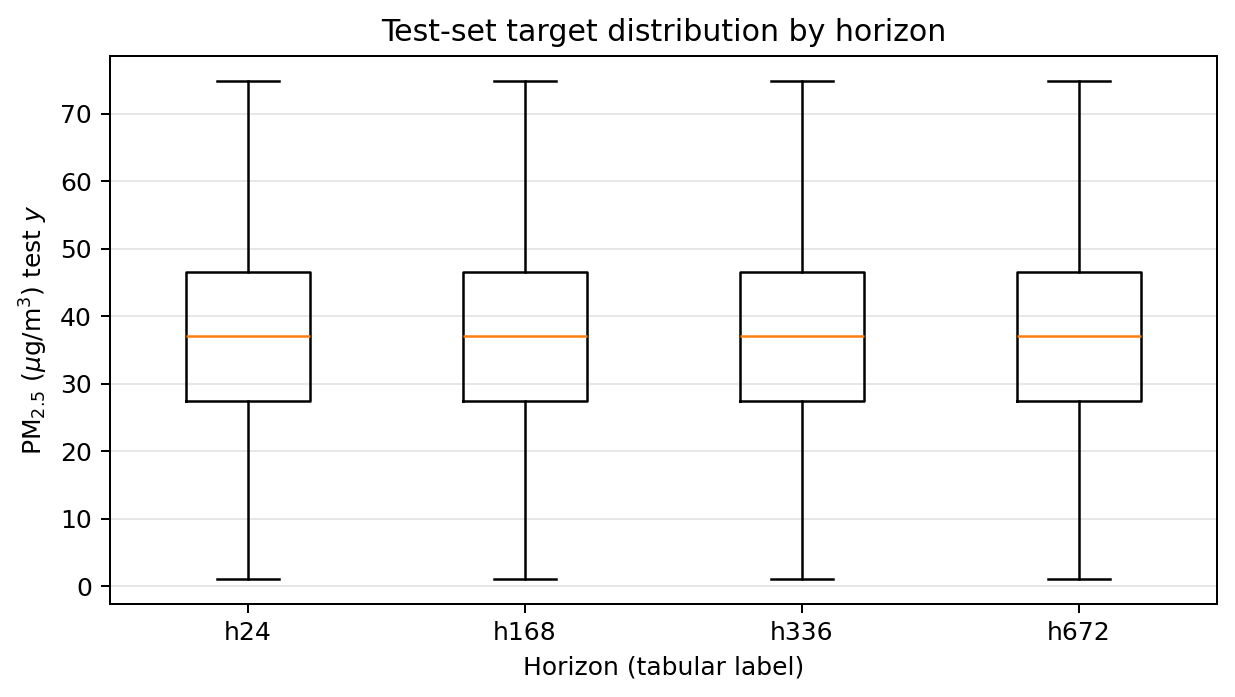
\includegraphics[width=0.70\textwidth]{figs/results_horizon_target_variability_box.png}%
%     \caption{Distribution of test-set forecast targets $y(t+H)$ by horizon (pooled 28-day test window). Identical boxplots reflect the same underlying test rows in this export, not necessarily equal difficulty at each $H$.}
%     \label{fig:horizon_variability}
% \end{figure}

% \begin{table}[H]
% \centering
% \caption{Pre-specified paired comparisons on aligned test rows. $\Delta$MAE is model~A minus model~B (negative favours A). 95\% CIs from the same moving-block bootstrap as Table~\ref{tab:forecast-summary}; ``CI excludes 0'' indicates the interval does not contain zero. Comparisons with mismatched row alignment (joint vs per-horizon at short horizons) are omitted.}
% \label{tab:significance}
% \resizebox{0.70\textwidth}{!}{%
% \begin{tabular}{llrrl}
% \toprule
% Comparison (A vs B) & Horizon & $\Delta$MAE & 95\% CI & CI excludes 0? \\
% \midrule
% \texttt{mh\_lstm\_mha} vs \texttt{mh\_lstm} & 7~d & $-3.70$ & [$-6.17$, $-0.71$] & Yes \\
% \texttt{mh\_lstm\_mha} vs \texttt{mh\_lstm} & 14~d & $-6.80$ & [$-8.79$, $-4.99$] & Yes \\
% \texttt{mh\_lstm\_mha} vs \texttt{mh\_lstm} & 24~h & $+0.63$ & [$-3.12$, $3.60$] & No \\
% \texttt{mh\_lstm\_mha} vs \texttt{mh\_lstm} & 28~d & $-1.36$ & [$-4.57$, $2.38$] & No \\
% \texttt{mh\_lstm} vs per-horizon lstm & 28~d & $+0.94$ & [$-0.53$, $2.45$] & No \\
% \texttt{mh\_lstm\_mha} vs Ridge AR+Fourier & 28~d & $-2.17$ & [$-5.15$, $-0.10$] & Yes \\
% \bottomrule
% \end{tabular}}
% \end{table}

% To complement pooled accuracy in Table~\ref{tab:forecast-summary}, Figure~\ref{fig:scatter_tabular_h24} shows \emph{point-level} test-set diagnostics for three tabular models at $H{=}24$~h only (Random Forest, linear SVR, XGBoost). Each row gives: (left) actual versus predicted PM$_{2.5}$ with the $y{=}x$ reference; (center) residuals versus predicted values; (right) actual and predicted series against label time on the held-out test window. These panels make systematic behaviour at moderate versus high concentrations visible in a way that scalar MAE/RMSE alone does not; we retain a single horizon here to avoid repeating the same message across figures.

% \begin{figure*}[!t]
%     \centering
%     \begin{subfigure}[b]{\textwidth}
%         \centering
%         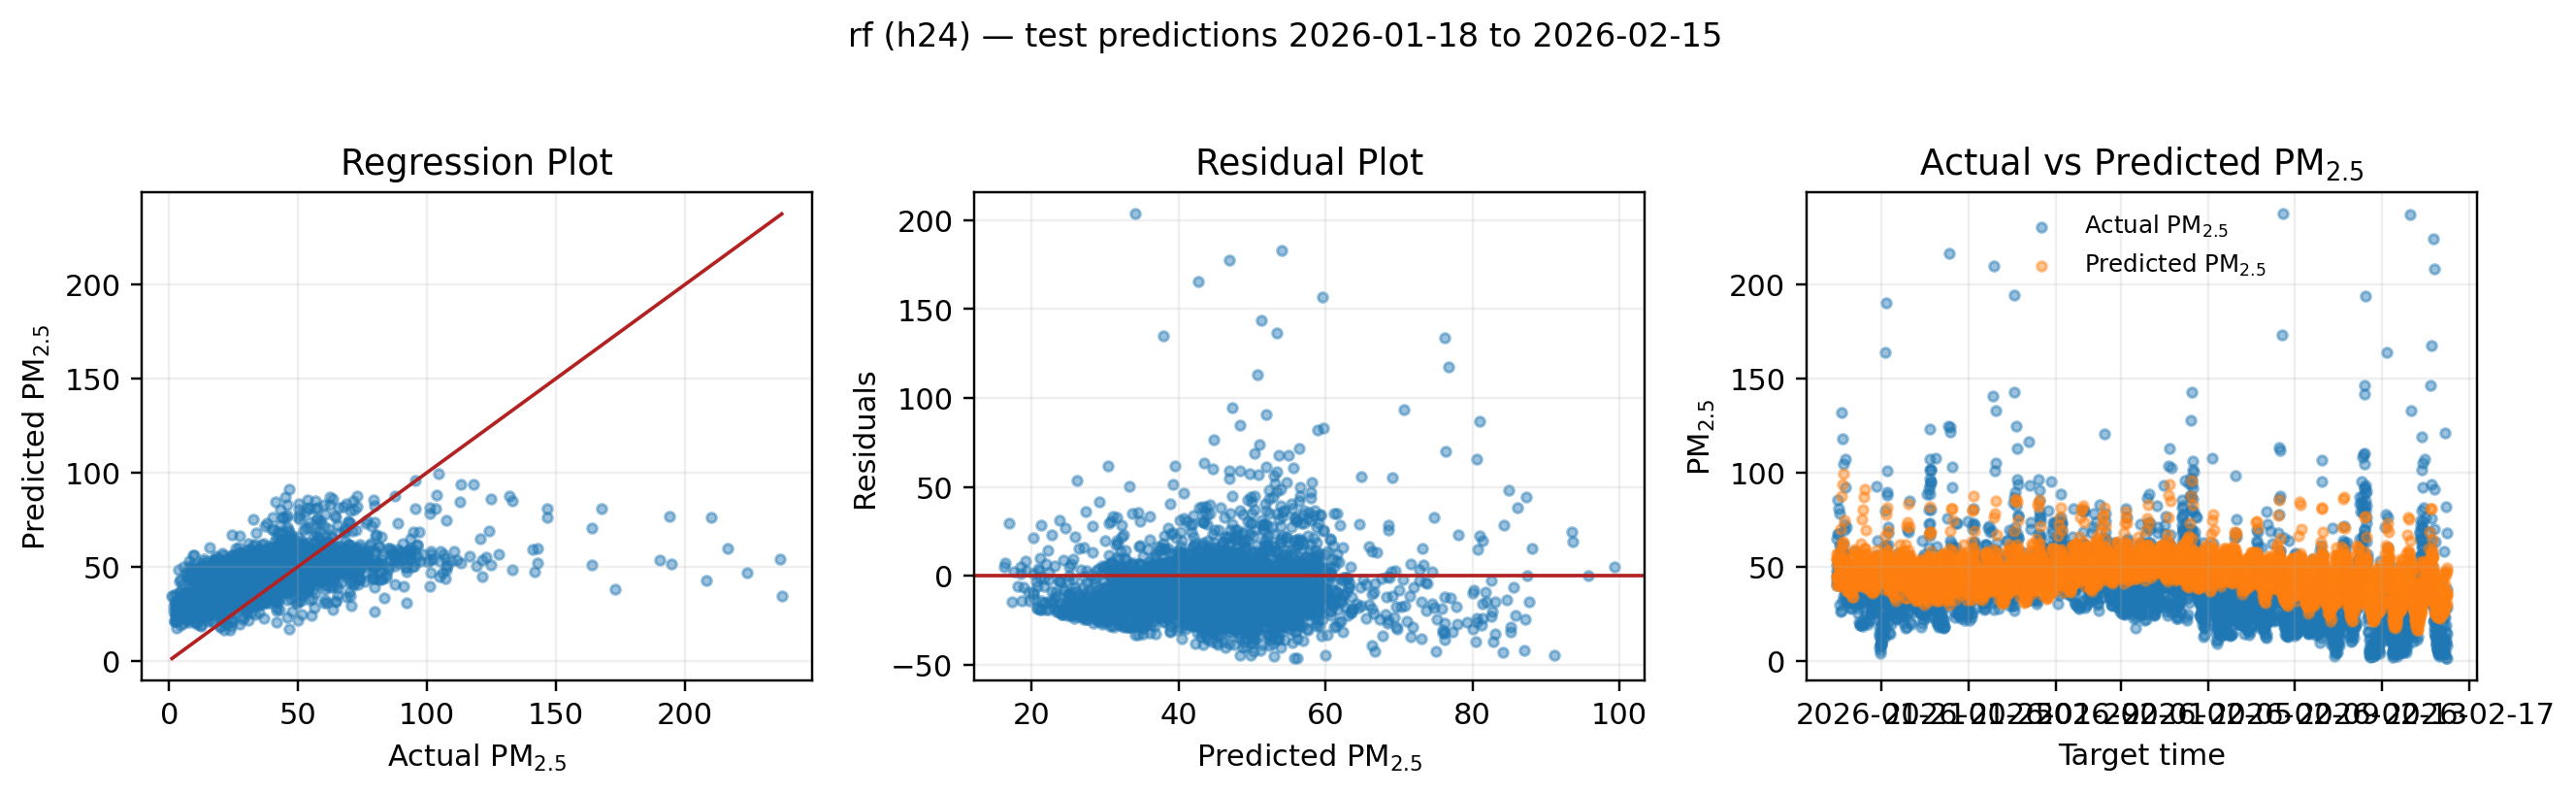
\includegraphics[width=0.95\textwidth]{figs/results_scatter_rf_h24.png}%
%         \caption{Random Forest (tabular lags).}
%     \end{subfigure}

%     \begin{subfigure}[b]{\textwidth}
%         \centering
%         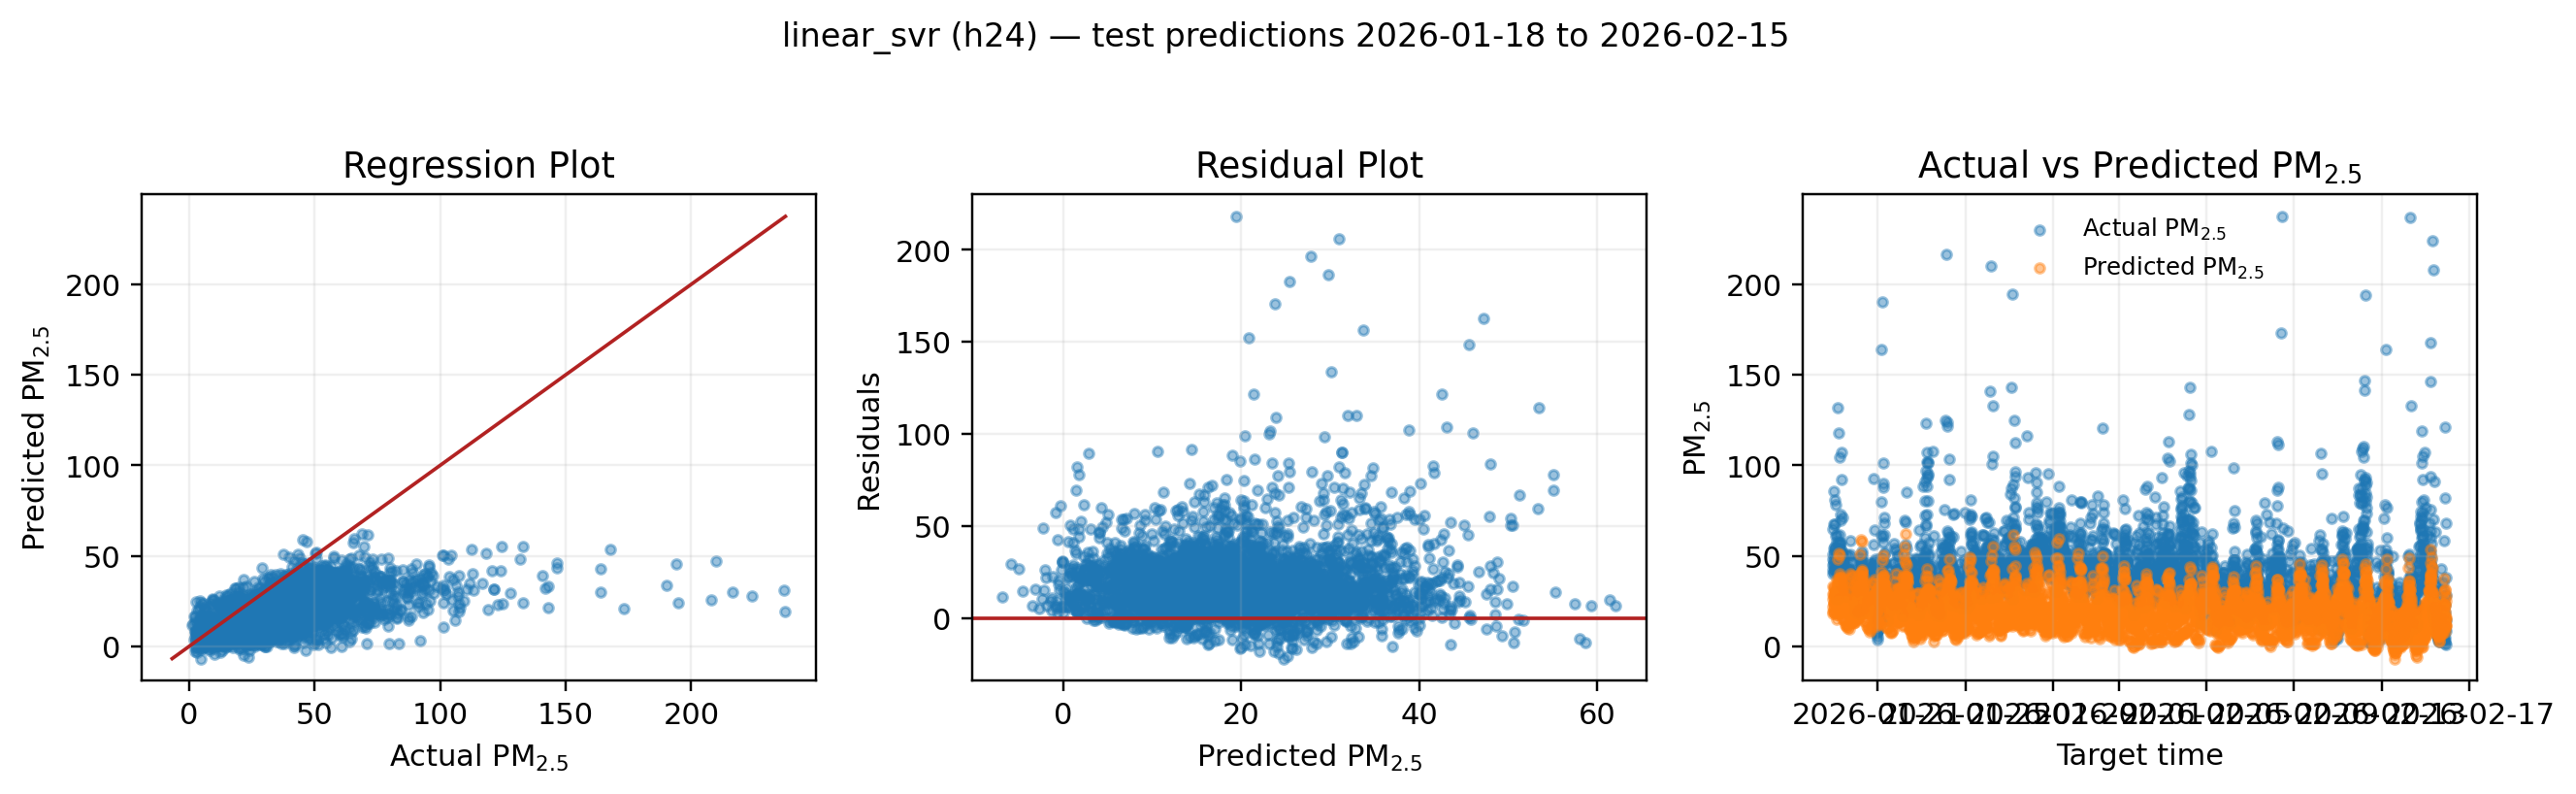
\includegraphics[width=0.95\textwidth]{figs/results_scatter_linear_svr_h24.png}%
%         \caption{Linear SVR (tabular lags).}
%     \end{subfigure}

%     \begin{subfigure}[b]{\textwidth}
%         \centering
%         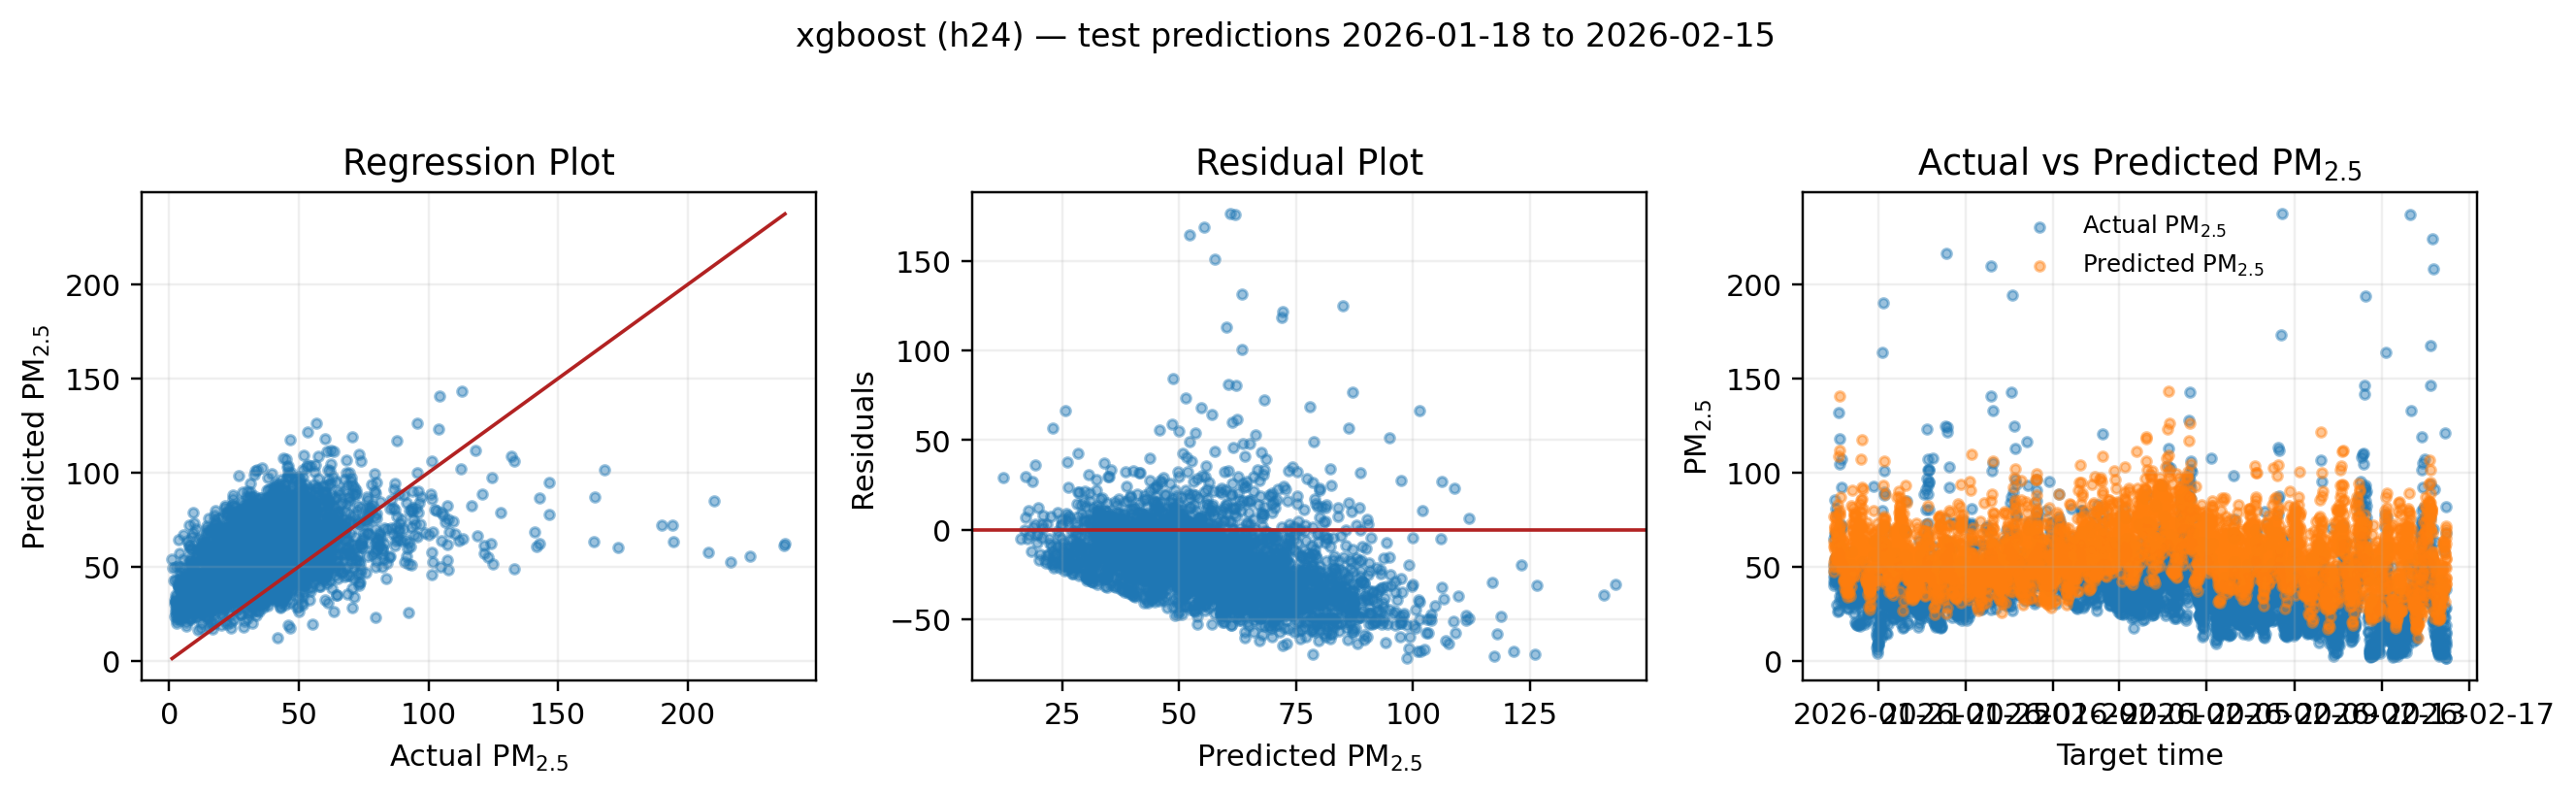
\includegraphics[width=0.95\textwidth]{figs/results_scatter_xgboost_h24.png}%
%         \caption{XGBoost (tabular lags).}
%     \end{subfigure}
%     \caption{Diagnostic scatter plots for direct 24~h forecasts on the pooled multi-site test split, using exported test predictions (\texttt{reports/predictions/}; script~10). The layout mirrors standard regression and residual views: departure from the diagonal at high concentrations indicates conditional bias in the upper tail; the time overlay highlights how point forecasts track the bulk trajectory but often smooth short-lived spikes.}
%     \label{fig:scatter_tabular_h24}
% \end{figure*}

% \begin{table}[H]
% \centering
% \caption{Forecast accuracy stratified by regime on a regime-spanning evaluation window (test window length increased to 84~days to include both pre-Harmattan and Harmattan periods). Values are MAE ($\mu$g/m$^3$) on the test set for simple benchmarks; this table is intended as a regime-aware diagnostic complementary to the primary 28-day test results in Table~\ref{tab:forecast-summary}.}
% \label{tab:forecast-regime}
% \resizebox{0.95\textwidth}{!}{%
% \begin{tabular}{llrrr}
% \toprule
% Horizon & Model & Overall MAE & Pre-Harmattan MAE & Harmattan MAE \\
% \midrule
% 24~h & Naïve level (persistence) & 12.59 & 10.40 & 12.84 \\
% 24~h & Seasonal naïve (weekly anchor) & 13.75 & 10.86 & 14.10 \\
% \midrule
% 7~d (168~h) & Naïve level (persistence) & 13.61 & 10.84 & 14.25 \\
% 7~d (168~h) & Seasonal naïve (weekly anchor) & 14.46 & 13.31 & 14.73 \\
% \bottomrule
% \end{tabular}}
% \end{table}

% \begin{table}[H]
% \centering
% \caption{Tabular models: test-set MAE ($\mu$g/m$^3$) stratified by Harmattan regime on an \textbf{84-day} label-time held-out window (both regimes present). The primary pooled scores in Table~\ref{tab:forecast-summary} use the standard \textbf{28-day} test and are not directly comparable row-for-row.}
% \label{tab:tabular-regime-mae}
% \resizebox{0.70\textwidth}{!}{%
% \begin{tabular}{llrrr}
% \toprule
% Horizon & Model & Overall MAE & Pre-Harmattan MAE & Harmattan MAE \\
% \midrule
% 24~h & Ridge AR+Fourier & 16.79 & 10.55 & 17.51 \\
% 24~h & Random Forest (tabular lags) & 10.33 & 7.89 & 10.61 \\
% 24~h & Linear SVR (tabular lags) & 14.61 & 9.77 & 15.17 \\
% 24~h & XGBoost (tabular lags) & 10.90 & 8.81 & 11.15 \\
% \midrule
% 7~d (168~h) & Ridge AR+Fourier & 35.25 & 12.19 & 40.40 \\
% 7~d (168~h) & Random Forest (tabular lags) & 12.01 & 8.56 & 12.78 \\
% 7~d (168~h) & Linear SVR (tabular lags) & 13.58 & 8.86 & 14.63 \\
% 7~d (168~h) & XGBoost (tabular lags) & 12.89 & 9.76 & 13.59 \\
% \midrule
% 14~d (336~h) & Ridge AR+Fourier & 48.80 & 34.82 & 54.06 \\
% 14~d (336~h) & Random Forest (tabular lags) & 11.73 & 9.85 & 12.44 \\
% 14~d (336~h) & Linear SVR (tabular lags) & 33.74 & 21.33 & 38.41 \\
% 14~d (336~h) & XGBoost (tabular lags) & 13.38 & 11.51 & 14.09 \\
% \midrule
% 28~d (672~h) & Ridge AR+Fourier & 63.08 & 27.13 & 93.17 \\
% 28~d (672~h) & Random Forest (tabular lags) & 13.04 & 10.86 & 14.87 \\
% 28~d (672~h) & Linear SVR (tabular lags) & 41.02 & 17.32 & 60.86 \\
% 28~d (672~h) & XGBoost (tabular lags) & 14.44 & 12.25 & 16.27 \\
% \bottomrule
% \end{tabular}}
% \end{table}

% \subsubsection{Short-term (24hr)}\label{sec:res24}
% At $H=24$~h, the lowest pooled MAE among models in Table~\ref{tab:forecast-summary} is achieved by the restricted Ridge AR+Fourier benchmark (11.96~$\mu$g/m$^3$; bootstrap 95\% CI [10.96, 12.98]), marginally below jointly trained sequence models (mh\_lstm: 12.31; mh\_lstm\_mha: 12.94). The per-horizon direct LSTM underperforms badly at this lead (MAE 23.19; $R^2<0$), illustrating that rankings are not stable across training paradigms in a short record. Paired tests do not show a significant advantage of joint attention over joint LSTM at 24~h (Table~\ref{tab:significance}). Spike hours remain difficult for all approaches: Ridge MAE$^{90}$~=~35.65~$\mu$g/m$^3$ versus pooled MAE 11.96 (Table~\ref{tab:forecast-upper-decile}), a $\approx$3$\times$ gap. Figure~\ref{fig:scatter_tabular_h24} illustrates how tabular models can track the bulk trajectory while smoothing short-lived high-concentration excursions. Harmattan-aware tabular diagnostics on an extended 84-day test window appear in Tables~\ref{tab:forecast-regime}--\ref{tab:tabular-regime-mae}; pooled MAE in Table~\ref{tab:tabular-regime-mae} is not directly comparable to Table~\ref{tab:forecast-summary} because of window length (and stochasticity in tree ensembles).

% \subsubsection{Mid-terms (7d and 14d)}\label{sec:res714}
% For $H=168$~h, the jointly trained attention model (\texttt{mh\_lstm\_mha}) achieves the lowest pooled MAE (11.32~$\mu$g/m$^3$; CI [9.68, 12.92]), outperforming the per-horizon LSTM (13.04), jointly trained mh\_lstm (15.02), and the weekly seasonal-na\"{i}ve comparator (15.39; Table~\ref{tab:forecast-summary}). Paired block-bootstrap inference supports a significant MAE reduction for mh\_lstm\_mha versus mh\_lstm at this horizon ($\Delta$MAE $\approx -3.7$~\textmu g/m$^3$; Table~\ref{tab:significance}). This suggests that, within this limited window, sharing supervision across horizons can improve medium-term generalisation when combined with attention, although upper-decile error remains much larger than pooled MAE (mh\_lstm\_mha MAE$^{90}$ 33.45 vs 11.32; Table~\ref{tab:forecast-upper-decile}).

% At $H=336$~h, mh\_lstm\_mha attains the strongest pooled accuracy in the experiment (MAE 9.78~$\mu$g/m$^3$; CI [8.69, 10.80]), beating tabular linear SVR (14.52) and per-horizon LSTM (14.31), with a statistically significant paired advantage over mh\_lstm ($\Delta$MAE $\approx -6.8$~\textmu g/m$^3$; Table~\ref{tab:significance}). This is the largest relative gain for joint attention in the study. We do not attribute the low 14~d pooled MAE solely to intrinsically ``easier'' targets in this window without longer records: Table~\ref{tab:horizon-variability} and Figure~\ref{fig:horizon_variability} show identical marginal target summaries across horizons in the current 28-day test export (same $n_{\mathrm{test}}$ and moments), so apparent ease at 14~d is not established by target variance alone. Nevertheless, the spike gap persists: MAE$^{90}$ at 14~d is 33.35~$\mu$g/m$^3$ for mh\_lstm\_mha ($\approx$3.4$\times$ pooled MAE).

% \subsubsection{Long-terms (28d)}\label{sec:res672}
% At $H=672$~h, mh\_lstm\_mha attains the lowest pooled MAE among listed models (13.56~$\mu$g/m$^3$; Table~\ref{tab:forecast-summary}), with a significant paired advantage over Ridge AR+Fourier at this lead ($\Delta$MAE $\approx -2.2$~\textmu g/m$^3$; Table~\ref{tab:significance}) but not over mh\_lstm. Pooled $R^2$ remains weakly positive (0.041), consistent with high episodic variance in a short test window. Per-horizon attention models remain unstable at long leads when trained independently. Upper-tail episodes remain systematically harder than pooled MAE (mh\_lstm\_mha MAE$^{90}$ 32.17; Table~\ref{tab:forecast-upper-decile}), consistent with the heavy-tailed distributions in Figure~\ref{fig:pm25_distribution}.

\section{Discussion}

This study examined PM$_{2.5}$ predictability across multiple forecast horizons under 
seasonal atmospheric variability in coastal Ghana. Three findings are particularly 
important. First, model ranking depended strongly on forecast horizon, and increased 
model complexity did not produce a uniform improvement in predictive accuracy. Second, 
Forecast performance was poorer during Harmattan conditions, indicating that model reliability varied across the observed atmospheric regimes. Third, average predictive accuracy did 
not fully represent model behaviour during high-pollution conditions, where substantially 
larger errors were observed for the attention-enhanced LSTM and several competing models. 
Together, these findings indicate that PM$_{2.5}$ forecasting should be evaluated as a 
horizon-, regime-, and event-dependent problem rather than using a single aggregate 
performance measure.

\subsection{Forecast horizon and the value of model complexity}

The comparison across forecasting horizons shows that the most appropriate modelling 
strategy depends on the temporal scale of prediction. At the 24-h horizon, Ridge 
AR+Fourier achieved the lowest pooled MAE, outperforming the more complex sequence 
models. This result indicates that short-term PM$_{2.5}$ dynamics in the study area 
contain substantial temporal persistence and recurrent structure that can be represented 
effectively using lagged observations and periodic temporal terms. The grouped predictor 
\orig{analysis supports this interpretation: lagged PM$_{2.5}$ variables accounted for the 
largest share of predictive importance, while particulate and temporal indicators also 
contributed substantially.}
\prop{analysis is consistent with this interpretation only as a validation permutation test: lagged PM$_{2.5}$ produced the largest $\Delta$MAE (0.74~$\mu$g\,m$^{-3}$; 5th--95th percentile 0.60--0.91), while collinear particulate lags received high impurity share but negative permutation $\Delta$MAE.}

The relative advantage of model classes changed at longer horizons. \orig{The joint 
multi-horizon LSTM with attention achieved the lowest pooled MAE at 7, 14 and 28 days. 
This result is consistent with the premise that shared sequence representations can 
become useful when prediction depends on temporal information distributed over longer 
historical windows. Joint multi-output forecasting allows related horizons to share a 
common representation rather than treating every lead time as an entirely independent}
\prop{The joint 
multi-horizon LSTM with attention achieved the lowest pooled MAE at 7 and 14 days. At 28 days it also had the lowest point-estimate MAE, but that ranking was not a statistically supported attention increment over the joint LSTM without attention, and the 28-day MAE interval overlapped those of Ridge AR+Fourier and Random Forest. 
The 7- and 14-day results are consistent with the premise that shared sequence representations can 
become useful when prediction depends on temporal information distributed over longer 
historical windows. They are not, however, a sample-size-matched comparison with tabular models (1{,}374 joint training sequences versus more than 13{,}000 tabular rows; 1{,}957 versus 4{,}037 test rows). Joint multi-output forecasting allows related horizons to share a 
common representation rather than treating every lead time as an entirely independent} 
problem, an advantage previously identified in multi-step forecasting research \citep{chevillon2007direct,raheja2023low}. Attention may further improve this representation by assigning greater weight to informative parts of the historical sequence rather than treating all encoded states equally \citep{vaswani2017attention,lim2021time}.

Importantly, however, the paired comparisons show that the benefit of attention was not 
uniform. Relative to the joint LSTM without attention, the reduction in MAE was 
statistically supported at 7 and 14 days, but not at 24 h or 28 days. This distinction is 
important because a lower pooled error alone does not establish that additional 
architectural complexity provides a robust improvement. The results therefore support a 
conditional rather than universal argument for attention-based forecasting: additional 
sequence complexity appears most useful at selected horizons where longer-range temporal 
dependencies contain exploitable predictive information.
\prop{The 24-h residual LSTM and the 28-day climatology blend that qualify those end-horizon results are reported in Section~\ref{sec:diagnostics}.}

The observed relationship between error and horizon was also non-monotonic. For the 
attention-enhanced joint model, the lowest pooled MAE occurred at 14 days rather than at 
24 h or 7 days, before increasing at 28 days. This pattern should not be interpreted as 
evidence that longer-horizon forecasting is intrinsically easier. \orig{Differences in target 
construction, available observations and the temporal composition of evaluation windows 
can influence errors across horizons. Instead, the results show that forecastability in}
\prop{The 14-day MAE interval was separated from the 24-h interval but overlapped the 7-day interval, so the 14- versus 7-day contrast is not strongly separated. Explained variance was higher at 7 days ($R^2=0.155$) than at 14 days ($R^2=0.108$), and MAE$^{90}$ remained about 33~$\mu$g\,m$^{-3}$ at both horizons, indicating a bulk rather than spike improvement. Joint sequences are keyed to the 28-day label time, so the four heads evaluate PM$_{2.5}$ at different clock times; the 14-day labels had a narrower central spread than the 24-h labels, but the same 14-day targets produced the worst MAE for the joint LSTM without attention. The 14-day minimum is therefore an architecture-specific empirical result, not evidence that the 14-day forecasting task is inherently more predictable. Instead, forecastability in} 
this dataset depends on how the prediction horizon interacts with temporal persistence, 
seasonal structure and model representation. This reinforces the value of evaluating 
environmental forecasting models across multiple operational horizons rather than 
extrapolating conclusions from a single lead time.

\subsection{\orig{Seasonal non-stationarity and Harmattan-related forecast degradation}\prop{Seasonal non-stationarity and calendar-defined Harmattan forecast degradation}}

The Harmattan analysis provides evidence that \orig{atmospheric regime is} \prop{a calendar-defined atmospheric period is} an important source of forecasting non-stationarity. \orig{Mean PM$_{2.5}$ increased from 25.77 to 31.19~$\mu$g\,m$^{-3}$ between the pre-Harmattan and Harmattan periods, while the median and upper distribution also shifted upward.} \prop{Pre-Harmattan is the record through 30~November~2025 and Harmattan is 1~December~2025--28~February~2026. Those dates are a calendar proxy, not a wind- or AOD-based regime classifier. Mean PM$_{2.5}$ increased from 25.77 to 31.19~$\mu$g\,m$^{-3}$ between those periods, while the median and upper distribution also shifted upward.} Elevated concentrations persisted across much of the diurnal cycle during Harmattan, indicating that the seasonal transition represented more than a short-lived increase in isolated pollution peaks. This shift is consistent with the influence of Saharan dust transport across West Africa \citep{afeti2000physical,crumeyrolle2019aerosol,amegah2022particulate,owusu2025spatiotemporal}. During Harmattan, regional mineral aerosol loading occurs alongside urban sources such as traffic, fuel combustion and industrial activity. Changes in atmospheric transport, mixing and deposition can therefore alter both the marginal distribution of PM$_{2.5}$ and the relationships between historical predictors and future concentrations \citep{crumeyrolle2019aerosol}. From a forecasting perspective, this means that relationships learned predominantly under one set of atmospheric conditions may not remain equally reliable after a seasonal transition.

\orig{The regime-stratified experiment supports this interpretation. Prediction errors were higher during Harmattan for the evaluated benchmark and tabular models, although the magnitude of degradation differed considerably among model classes.}
\prop{The regime-stratified experiment supports this interpretation only in part. Headline joint models ($L=1{,}344$~h; 56-day lookback) remain absent from the 84-day split and therefore cannot be treated as seasonally validated. A separate 14-day-lookback joint run ($L=336$~h; $n_{\mathrm{train}}=564$) shows Harmattan MAE rising for vanilla joint LSTM at all four horizons, while joint attention was unstable at 7~d. That short-lookback run is not a direct validation of the headline 56-day encoder. For the evaluated benchmark and tabular models, prediction errors were higher during Harmattan, although the magnitude of degradation differed considerably among model classes.} Random Forest was comparatively stable across the regime-spanning evaluation window, with its mean MAE across the four horizons increasing from 9.29 to 12.68~$\mu$g\,m$^{-3}$, corresponding to a 36.4\% increase. In contrast, Ridge AR+Fourier deteriorated sharply at longer 
horizons, while Linear SVR also showed substantial degradation at 28 days. These differences indicate that \orig{environmental regime change}\prop{the calendar-defined Harmattan period} does not affect all forecasting architectures equally. The poor longer-horizon performance of some models under Harmattan may reflect a loss of stability in relationships learned from historical lags and regular temporal cycles. A model can exploit persistent patterns effectively when the generating process remains relatively stable, yet perform poorly when external atmospheric forcing changes those relationships. The results therefore suggest that model evaluation based only on a single pooled test period can overstate expected robustness in environments characterised by strong seasonal transitions.

For environmental forecasting systems in regions affected by Harmattan, \orig{regime-aware evaluation}\prop{evaluation across calendar-defined seasonal periods} should therefore be considered part of model validation rather than an optional secondary analysis. Longer datasets covering multiple Harmattan cycles would also allow future work to examine whether season-specific models, adaptive retraining, regime indicators or mixture-of-experts approaches can improve stability when atmospheric conditions change. \prop{With only one observed Harmattan transition, the present regime results are associations in this sample, not repeated seasonal validation.}

\subsection{Forecast reliability during high-pollution conditions}

The upper-tail analysis provides a second indication that aggregate forecasting accuracy 
does not completely characterise model reliability. For the attention-enhanced joint 
LSTM, MAE increased substantially when evaluation was restricted to observations at or 
above the 90th percentile of observed PM$_{2.5}$. At 24 h, for example, pooled MAE was 
12.94~$\mu$g\,m$^{-3}$ compared with an upper-tail MAE of 
28.95~$\mu$g\,m$^{-3}$. Corresponding upper-tail errors were 
33.45, 33.35 and 32.17~$\mu$g\,m$^{-3}$ at the 7-, 14- and 28-day horizons, 
respectively. \prop{Those headline MAE$^{90}$ values use a pooled $Q_{0.90}$. Site-specific 24-h thresholds (Table~\ref{tab:mae90-by-site}) show that pooled tails over-weight high-mean schools and that several joint site tails have $n_{90}<20$.}

A similar increase was observed for several competing models, although the relationship between pooled and upper-tail error was model-dependent. Random Forest, Ridge 
AR+Fourier and the LSTM variants generally produced substantially larger errors during high-concentration observations, whereas this pattern was not present for every model--horizon combination. This heterogeneity is important because it shows that upper-tail performance cannot be inferred directly from average MAE.
The 24-h diagnostic plots provide additional evidence of this problem. Random Forest and XGBoost reproduced the broader temporal pattern reasonably well, but abrupt pollution peaks were frequently smoothed or underestimated, while residual dispersion increased at higher concentrations, particularly for Linear SVR. Regression models optimised for global predictive performance may favour well-represented regions of the target distribution, resulting in poorer predictive performance for rare and extreme observations \citep{ribeiro2020imbalanced,diekuu2025mitigating}

This result has practical implications for air-quality forecasting. High-concentration episodes are precisely the conditions under which advance information may be most useful for exposure management. A model with a favourable overall MAE may therefore remain insufficiently reliable for event-based warning applications. Future evaluation should extend beyond conventional MAE and RMSE to include exceedance-event detection, 
probabilistic calibration, prediction intervals and tail-specific scoring. Weighted or asymmetric loss functions may also be useful where errors during hazardous pollution conditions carry greater decision costs than errors during routine conditions \citep{koenker1978regression}.

\subsection{Environmental variability and predictor structure}

The forecasting results should also be interpreted in the context of the substantial environmental heterogeneity observed across the monitoring network. Mean PM$_{2.5}$ concentrations varied markedly among sites, ranging from approximately 19.12~$\mu$g\,m$^{-3}$ at Tema Community 25 Estate to 
35.15~$\mu$g\,m$^{-3}$ at Divine Healer's Church, with Satet International School also recording comparatively high concentrations. Approximately 69\% of observations exceeded the WHO daily PM$_{2.5}$ guideline, indicating that elevated particulate concentrations were common rather than restricted to isolated episodes.

Differences among school, residential and port-related locations point to substantial spatial heterogeneity in exposure. These variations may reflect differences in surrounding traffic, land use, local combustion sources, dust resuspension and industrial activity \citep{hodoli2025urban,amegah2022particulate}, although the present monitoring design does not permit individual emission sources to be attributed causally. The pronounced morning concentration peak and lower midday values are also consistent with interactions between temporally structured emissions and 
boundary-layer development \cite{crumeyrolle2019aerosol,lu2021estimating}.

The grouped predictor analysis provides a modelling perspective on these environmental patterns. \orig{Lagged PM$_{2.5}$ variables contributed 27.64\% of total importance, followed by particulate indicators at 22.12\% and temporal variables at 15.78\%. Meteorological conditions accounted for 10.40\%, spatial factors for 8.12\%, CO$_2$ for 6.63\%, and other environmental variables for 9.31\%. The dominance of historical PM$_{2.5}$ and related particulate measurements is consistent with the competitive performance of autoregressive models at short horizons and indicates substantial atmospheric memory in}
\prop{Grouped permutation on the 24-h Random Forest raised validation MAE by 0.74~$\mu$g\,m$^{-3}$ (0.60--0.91) when lagged PM$_{2.5}$ was shuffled, versus 0.25 for meteorology and 0.10 for CO$_2$. Impurity importance over-weighted other particulate lags (41.5\% MDI) that permutation showed were redundant: additional particulate indicators may provide limited incremental predictive information after historical PM$_{2.5}$ is already available. These are predictive contributions on one validation window, not causal shares. The dominance of historical PM$_{2.5}$ is consistent with the competitive performance of autoregressive models at short horizons and indicates substantial atmospheric memory in} 
the observed series.

At the same time, the contributions from temporal, meteorological and spatial variables show that persistence alone does not explain PM$_{2.5}$ variability. Seasonal cycles, site-specific conditions and meteorological processes provide additional information, which becomes especially relevant when atmospheric conditions depart from their recent history. The decline in model stability during Harmattan reinforces this point: strong historical predictors can support accurate forecasts under relatively stable conditions, but their relationships with future concentrations may weaken when regional atmospheric 
forcing changes.

\subsection{Implications for environmental forecasting in data-constrained settings}

The findings have broader implications for environmental modelling in cities where monitoring records are relatively short and operational air-quality forecasting remains limited. First, model selection should be horizon-specific. The strong 24-h performance of Ridge AR+Fourier shows that computationally simpler models should not be displaced by deep learning solely because more complex architectures are available. Where recent observations and recurrent temporal structure dominate the predictive signal, transparent 
statistical models may provide comparable or better performance at substantially lower computational cost.

Second, the value of more complex sequence models should be demonstrated empirically. In this study, joint attention-based learning provided clear advantages at selected medium-to-long horizons, but not uniformly across all horizons. A practical forecasting system could therefore employ different model classes for different lead times rather than relying on a single architecture for every forecasting objective.

Third, validation under \orig{environmental regime change}\prop{a calendar-defined Harmattan period} should form part of model development. The Harmattan experiment showed that pooled accuracy alone can conceal substantial degradation under seasonally altered atmospheric conditions. For African cities affected by dust transport and other strong seasonal processes, model validation should therefore include regime-stratified errors and uncertainty estimates.

Finally, the results support the potential value of combining low-cost monitoring networks with forecasting models in settings where conventional monitoring infrastructure is sparse \citep{attey2025utility,hodoli2024urban}. However, the present analysis should be viewed as a modelling evaluation rather than validation of an operational warning system. Before forecasts can support routine pollution advisories, they require longer-term evaluation, threshold-based event assessment, uncertainty calibration, external validation and testing under multiple 
seasonal cycles.

\subsection{Limitations and future research}

Several limitations should be considered when interpreting the results. \orig{First, the observational period covers approximately six months and therefore represents a relatively short record for long-horizon sequence modelling. Although the dataset includes both pre-Harmattan and Harmattan conditions, only one Harmattan transition was observed. Consequently, the stability of model rankings and the magnitude of regime-related degradation cannot yet be assumed to generalise across years.} \prop{First, this is a short-record empirical forecasting study. The observational period covers approximately six months and is a short record for 28-day forecasting with a 56-day lookback. The dataset includes one pre-Harmattan period, one Harmattan period and one seasonal transition. Model rankings and calendar-period error changes therefore cannot be assumed to generalise across years, and the 28-day results are within-sample comparisons rather than evidence of general long-term PM$_{2.5}$ forecastability in coastal Ghana.}

Second, the analysis is geographically restricted to seven monitoring locations within coastal Greater Accra. \prop{All seven appear in the descriptive analysis; headline forecast scores use the six sites with eligible 28-day test rows (Table~\ref{tab:site-availability}).} The sites capture different school, residential and industrial environments, but external validation is required before the reported model behaviour can be assumed to apply to other Ghanaian or West African cities.

Third, predictions were based primarily on observed historical environmental variables. Longer-horizon PM$_{2.5}$ prediction may benefit from incorporating forecast meteorology, regional dust indicators, satellite aerosol products and large-scale atmospheric circulation information. Such variables could provide forward-looking information that historical pollutant lags alone cannot supply when atmospheric regimes change.

Fourth, the study evaluates deterministic point forecasts. The increased errors observed during Harmattan and upper-tail pollution conditions indicate that probabilistic forecasting may provide a more useful representation of uncertainty. Future work should therefore investigate prediction intervals, quantile forecasting, probabilistic sequence models and tail-aware objectives.

\prop{Fifth, hyperparameters for the headline tables were specified a priori. A 24-h validation check (Table~\ref{tab:hp-sens}) found Random Forest insensitive to 200 versus 600 trees and slightly better with leaf size 5 than 3. A 24-h direct-LSTM lookback and width check (Table~\ref{tab:lstm-h24-sens}) supported the headline architecture. Attention-head count, joint models, other horizons and the learning rate were held fixed. A residual 24-h LSTM and a 28-day attention--climatology blend (three fixed $\alpha$, not tuned) are robustness checks only (Section~\ref{sec:diagnostics}); headline tables remain unblended models.}

Sixth, joint models used 1{,}374 training sequences versus 13{,}263--17{,}285 tabular rows, and 1{,}957 rather than 4{,}037 test rows. Unpaired MAE comparisons across families are therefore not sample-size or row-matched except where paired tests were possible.

Seventh, \prop{the Harmattan robustness check is a separate 14-day-lookback ($L=336$~h) experiment and is not a direct validation of the headline 56-day model. That 56-day encoder still cannot be trained on the 84-day split; the substitute run uses only 564 training sequences, and joint attention was unstable at 7~d on that run (overall MAE 33.15).}

Eighth, headline MAE$^{90}$ uses a pooled $Q_{0.90}$. Site-specific tails at 24~h--28~d (Tables~\ref{tab:mae90-by-site}--\ref{tab:mae90-by-site-mha}) show that this threshold is not representative of cleaner sites, and several joint site tails have $n_{90}<20$.

Ninth, grouped permutation importance is reported for the 24-h Random Forest only. SHAP values were not computed.

\orig{Finally, low-cost sensor observations remain subject to measurement and calibration uncertainty \citep{raheja2023low}. Although corrected PM$_{2.5}$ values were used in the present analysis, future work should quantify how sensor-correction uncertainty propagates into forecast uncertainty. Longer multi-season records, independent spatial validation and explicit evaluation of high-pollution event detection will be important steps toward establishing whether these models can support reliable operational air-quality forecasting.}
\prop{Finally, low-cost sensor observations remain subject to measurement and calibration uncertainty \citep{raheja2023low}. Although corrected PM$_{2.5}$ values were used in the present analysis, future work should quantify how sensor-correction uncertainty propagates into forecast uncertainty. Longer multi-season records, a headline-lookback joint regime experiment, LSTM sweeps at other horizons and of attention, SHAP importances, independent spatial validation and explicit evaluation of high-pollution event detection will be important steps toward establishing whether these models can support reliable operational air-quality forecasting.}

% \section{Discussion}\label{sec4}

% \subsection{Spatiotemporal characteristics of PM$_{2.5}$ in coastal Accra}

% The findings reveal substantial spatiotemporal heterogeneity in PM$_{2.5}$ concentrations across coastal communities in the Greater Accra region, reflecting the combined influence of local emissions, land-use patterns, and regional atmospheric processes. Mean PM${2.5}$ concentrations consistently exceeded World Health Organization guideline thresholds, indicating persistent exposure risk across locations. The observed positive skewness across sites further suggests that urban particulate pollution in coastal Accra is not characterized by stable background concentrations but rather by intermittent high-concentration episodes, likely associated with short-term emission events and meteorological stagnation \cite{kang2018air}.

% A pronounced seasonal intensification of PM$_{2.5}$ was observed during Harmattan, with elevated concentrations recorded across nearly all hours of the day. This pattern is consistent with the well-documented role of long-range Saharan dust transport in increasing particulate loading across West Africa. During Harmattan, dry northeasterly winds transport mineral aerosols over long distances while reduced humidity and weakened wet deposition favor prolonged atmospheric residence of suspended particles. The persistence of elevated midday concentrations during the Harmattan suggests that regional dust loading interacted with local urban emissions, resulting in sustained exposure rather than isolated peaks. This finding underscores the importance of accounting for both regional atmospheric transport and local emission sources when assessing urban air quality in coastal Ghana.

% Marked differences between monitoring locations further indicate the importance of microenvironmental factors in shaping pollution exposure. School environments and densely populated community sites exhibited substantial variability in PM$_{2.5}$ concentrations, possibly reflecting fluctuations in nearby traffic density, roadside dust resuspension, open waste burning, and localized fuel combustion. Industrial and port-adjacent locations displayed more sustained concentration profiles, consistent with continuous emissions from transport logistics, shipping activity, fuel handling, and industrial operations. Such spatial variation highlights how land use and proximity to emission sources shape exposure inequalities within rapidly urbanizing cities.

% Distinct diurnal patterns provide additional insight into the environmental processes governing urban PM$_{2.5}$ dynamics. Morning peaks between 05:00 and 07:00 coincide with intensified commuter activity, commercial transport, and cooking-related combustion. Shallow atmospheric boundary layers during early morning hours may further restrict pollutant dispersion and enhance accumulation near the surface \cite{wang2019vertical}. Concentrations generally declined during midday, likely due to increased atmospheric mixing and boundary-layer expansion, before rising again during evening activity periods \cite{lv2020meteorological}. These recurrent patterns indicate strong interactions between anthropogenic emissions and atmospheric processes in determining daily pollution cycles.

% % The results reveal substantial spatiotemporal heterogeneity in PM${2.5}$ concentrations across the seven monitoring locations in coastal Accra. Mean corrected PM${2.5}$ concentrations ranged from approximately 19 to 35 $\mu$g/m$^3$, consistently exceeding World Health Organization guideline thresholds and indicating persistent exposure risk across communities. Divine Healer’s Church and Satet International School recorded the highest concentrations and widest distributions, while Tema Community 25 Estate exhibited comparatively lower levels. Positive skewness was evident across all sites, confirming that PM$_{2.5}$ concentrations were characterized by episodic high-pollution events rather than stable symmetric variation.
% % A pronounced seasonal intensification of PM${2.5}$ was observed during the Harmattan period. Diurnal analysis showed substantially higher median concentrations during Harmattan conditions than during pre-Harmattan periods at nearly all hours of the day. For example, midday PM${2.5}$ concentrations during Harmattan remained elevated (approximately 23–26 $\mu$g/m$^3$) compared with pre-Harmattan conditions (approximately 8–12 $\mu$g/m$^3$), while morning peaks increased to around 50 $\mu$g/m$^3$ near 06:00. These findings are consistent with the role of Saharan dust transport and reduced atmospheric dispersion during Harmattan in elevating particulate concentrations across West African cities.

% % Differences between monitoring locations further indicate localized emission effects. School and community sites exhibited considerable variability in PM$_{2.5}$ concentrations, likely reflecting differences in road traffic, dust resuspension, and local combustion activities. Port-adjacent and industrial areas displayed sustained pollution burdens, consistent with transportation and industrial emissions. Diurnal profiles revealed strong morning peaks around 05:00–07:00 and lower afternoon concentrations, suggesting interactions between commuter activity, atmospheric boundary-layer dynamics, and human activity patterns. The evening rise in concentrations further indicates recurring anthropogenic contributions to urban particulate pollution.

% \subsection{Drivers of PM$_{2.5}$ variability and predictor importance}

% Results from the Random Forest feature importance analysis (Table~\ref{tab:feature_importance}) indicate that particulate persistence and particle abundance were dominant drivers of PM$_{2.5}$ variability in coastal Accra. The 0.3~$\mu$m particle count emerged as the strongest predictor, accounting for approximately 82.6\% of the total model importance, substantially exceeding that of all other variables. This finding suggests that fine particulate dynamics in the study area are strongly governed by local aerosol loading and short-term persistence in atmospheric particle concentrations. Such persistence is expected in urban environments characterized by repeated traffic emissions, industrial activity, domestic combustion, and seasonal dust transport, where preceding pollution conditions exert substantial influence on subsequent air quality \cite{leon2021pm}. The competitive performance of autoregressive models at shorter forecasting horizons further reinforces the importance of temporal memory in PM$_{2.5}$ dynamics.

% Spatial variability also contributed meaningfully to the prediction of PM$_{2.5}$. Encoded monitoring location was the second most important predictor (6.8\%), reflecting marked heterogeneity in pollution exposure across coastal communities. This finding is consistent with observed differences between school, residential, and port-adjacent environments, where local emission intensity, traffic activity, industrial operations, and proximity to pollution sources influence particulate concentrations. Day of year (4.1\%) also contributed substantially, indicating that seasonal atmospheric forcing, including Harmattan dust transport, plays an important role in shaping PM$_{2.5}$ variability across the study area.

% Meteorological and combustion-related indicators played a secondary, though environmentally meaningful, role in forecasting performance. Corrected CO$_2$ concentration contributed 3.8\% to predictive importance, suggesting that combustion-related activities, including vehicular movement and fossil fuel use, influence local particulate accumulation. Temperature had a smaller but measurable effect (0.8\%), likely through its influence on atmospheric mixing, pollutant dispersion, and aerosol formation. Forecast degradation during Harmattan further demonstrates the sensitivity of PM$_{2.5}$ dynamics to seasonal atmospheric forcing. Harmattan introduces abrupt shifts in aerosol composition, atmospheric stability, and regional transport patterns, thereby altering pollutant concentrations beyond locally generated emissions \cite{afeti2000physical,weinstein2010characterization}. The comparatively weaker model performance during Harmattan, therefore, reflects the difficulty of modeling abrupt environmental regime shifts driven by external atmospheric processes.

% Temporal variables further contributed to predictive performance by capturing recurrent behavioral and environmental cycles. Month (0.45\%), hour of day (0.42\%), and day of week (0.29\%) collectively indicate that PM$_{2.5}$ variability is shaped by regular human activity patterns, including commuting, commercial operations, and domestic combustion. The strong diurnal structure observed across locations, particularly morning and evening peaks, supports the role of temporally structured anthropogenic activity in driving particulate concentrations \cite{wang2019vertical}. Although NOX index (0.23\%) and site openness (0.06\%) contributed comparatively little, their inclusion may still reflect localized combustion and ventilation effects. Overall, these findings suggest that PM$_{2.5}$ dynamics in coastal Accra arise from interactions among particulate persistence, spatial heterogeneity, seasonal atmospheric forcing, combustion-related emissions, and temporally structured human activity.

% % The forecasting results suggest that particulate persistence was a dominant driver of PM$_{2.5}$ variability in coastal Accra. The strong performance of autoregressive approaches at shorter horizons indicates that recent pollution conditions contain substantial predictive information regarding near-future concentrations. This persistence likely reflects cumulative pollutant build-up from repeated daily emissions, combined with relatively slow atmospheric removal under stable urban conditions \cite{leon2021pm}. In environments characterized by recurrent traffic emissions, industrial activity, and seasonal dust transport, pollutant concentrations often exhibit temporal memory, whereby preceding conditions strongly shape subsequent air quality.

% % Meteorological processes also played an important, though secondary, role in shaping PM$_{2.5}$ dynamics. Forecast degradation during Harmattan demonstrates the sensitivity of urban pollution patterns to seasonal atmospheric forcing. Harmattan introduces abrupt shifts in aerosol composition, atmospheric stability, and regional transport dynamics, thereby altering pollutant distributions beyond locally driven emission patterns \cite{afeti2000physical,weinstein2010characterization}. Variables such as temperature, CO$_2$, and humidity likely influenced pollutant dispersion, aerosol formation, and deposition processes, even if their predictive contributions were smaller than those of particulate persistence \cite{leon2021pm}. The comparatively poorer model performance during Harmattan, therefore, reflects the difficulty of modeling abrupt regime changes driven by external atmospheric processes.

% % Temporal variables further contributed to predictive performance by capturing recurrent behavioral and environmental cycles. The strong diurnal structure observed across locations suggests that PM$_{2.5}$ variability is closely linked to regular human activity patterns, including commuting, commercial operations, and domestic fuel use \cite{wang2019vertical}. Seasonal indicators also contributed by representing longer environmental memory associated with Harmattan transitions and recurrent meteorological conditions. These findings reinforce the notion that PM$_{2.5}$ in urban Ghana is governed by interactions among anthropogenic emissions, seasonal atmospheric forcing, and temporally structured human activity.


% \subsection{Performance of multi-horizon forecasting models}
% Forecast performance varied considerably across prediction horizons, reflecting differences in the temporal complexity of urban air pollution processes. At shorter horizons, autoregressive and seasonal methods performed competitively, indicating that near-term PM$_{2.5}$ variability is strongly shaped by recent atmospheric conditions and recurring daily emission cycles. Similar observations have been reported in urban forecasting studies where short-term pollution is dominated by temporal persistence and routine human activity \cite{zheng2016design}.

% At medium-term horizons, attention-enhanced LSTM models demonstrated promising predictive capability, particularly under joint multi-horizon learning. Urban PM$_{2.5}$ concentrations are shaped by interacting processes occurring across multiple temporal scales, including traffic emissions, boundary-layer dynamics, and seasonal dust transport. Attention mechanisms likely improved representation of these complex dependencies by prioritizing informative historical periods \cite{abbasimehr2022improving,vaswani2017attention}.

% % At medium-term horizons, however, attention-enhanced LSTM models showed promising predictive capability, particularly under joint multi-horizon learning. These improvements likely reflect the ability of attention mechanisms to prioritize temporally informative historical periods, including seasonal transitions and repeated pollution cycles. Urban PM$_{2.5}$ concentrations are shaped by interacting processes occurring across multiple temporal scales, ranging from hourly traffic emissions to multi-day atmospheric transport and seasonal Harmattan influences. By selectively weighting relevant historical information, attention-enhanced models appear better suited to represent these complex temporal dependencies.

% Forecasting accuracy generally declined at longer horizons, consistent with increasing uncertainty in meteorological conditions, episodic emissions, and atmospheric transport processes. Longer-term forecasts are inherently more difficult because they depend on dynamic environmental systems influenced by both predictable seasonal cycles and stochastic disturbances \cite{zheng2016design}. The weaker performance at 28 days, therefore, likely reflects the cumulative uncertainty introduced by changing atmospheric conditions, irregular emission events, and regime shifts associated with Harmattan onset and intensity.

% % Model performance varied substantially across prediction horizons. At the short-term 24 h horizon, the restricted Ridge AR+Fourier model achieved the lowest pooled MAE (11.96 $\mu$g/m$^3$), marginally outperforming jointly trained LSTM models. This suggests that short-term PM$_{2.5}$ forecasting in data-constrained settings may be adequately represented by autoregressive and seasonal patterns without requiring complex deep-learning architectures. In contrast, the per-horizon direct LSTM performed poorly at 24 h (MAE = 23.19 $\mu$g/m$^3$; $R^2 < 0$), indicating instability when horizons are modeled independently within a short observational record.

% % At medium horizons, however, attention-enhanced joint sequence models demonstrated clear advantages. The joint LSTM with attention achieved the lowest pooled MAE at both 7 d (11.32 $\mu$g/m$^3$) and 14 d (9.78 $\mu$g/m$^3$), significantly outperforming joint LSTM models without attention. Paired block-bootstrap testing confirmed statistically significant improvements at 7 d ($\Delta$MAE $\approx -3.7$ $\mu$g/m$^3$) and 14 d ($\Delta$MAE $\approx -6.8$ $\mu$g/m$^3$). These findings suggest that attention mechanisms become particularly valuable when models are trained jointly across multiple horizons, enabling selective weighting of informative historical periods and improved representation sharing across forecast intervals.

% % Performance generally weakened at longer horizons, reflecting increased uncertainty associated with meteorological fluctuations, episodic emissions, and seasonal shifts. Although the joint LSTM with attention remained the best-performing sequence model at 28 d (MAE = 13.56 $\mu$g/m$^3$), predictive strength declined ($R^2 = 0.041$), suggesting that long-term PM$_{2.5}$ forecasting remains inherently difficult in rapidly changing urban environments. Nevertheless, the significant advantage over Ridge AR+Fourier at 28 d indicates that deep sequence learning provides meaningful gains when longer-range dependencies become more important.

% \subsection{Forecasting extreme pollution episodes and public health relevance}
% Extreme pollution episodes remained substantially more difficult to predict than average conditions, as reflected by elevated MAE$^{90}$ values across all horizons. This finding likely reflects the episodic nature of urban pollution in coastal Ghana, where abrupt changes in traffic congestion, open burning, industrial activity, and Harmattan dust intrusions may rapidly alter particulate concentrations. Such events often emerge from interactions between local emissions and transient atmospheric conditions, making them inherently difficult to anticipate using models optimized primarily for average prediction accuracy.

% From an environmental health perspective, these forecasting limitations are important because short-term PM$_{2.5}$ spikes often pose the greatest health risks. Acute exposure to elevated particulate concentrations has been linked to asthma exacerbations, COPD symptoms, cardiovascular stress, and increased respiratory healthcare demand \cite{liu2022pm2,xing2016impact}. In school environments and densely populated communities, anticipating hazardous pollution periods may support temporary measures to reduce exposure, such as behavioral advisories and adjustments to outdoor activities.

% Despite reduced performance during extreme events, the results demonstrate that predictive models can provide a useful early indication of elevated pollution risk in data-constrained settings. Operational forecasting systems that integrate low-cost sensor networks with predictive analytics may therefore offer a practical approach for strengthening air quality surveillance and public health preparedness in rapidly urbanizing African cities.

% % Despite improvements in pooled forecasting accuracy, extreme pollution episodes remained difficult to predict across all models. Upper-decile errors (MAE$^{90}$) were consistently three to four times larger than pooled MAE, highlighting persistent challenges in forecasting hazardous pollution spikes. For example, at 14 d the best-performing model achieved a pooled MAE of 9.78 $\mu$g/m$^3$, yet MAE$^{90}$ increased to 33.35 $\mu$g/m$^3$. Similar patterns were observed across all horizons, indicating that rare but severe pollution episodes remain poorly captured by standard prediction objectives.

% % The difficulty in forecasting spikes likely reflects the episodic nature of urban pollution in coastal Ghana, where traffic congestion, local combustion, industrial emissions, and sudden Harmattan dust intrusions may cause abrupt distributional shifts. Standard forecasting objectives primarily optimize average error and therefore place less emphasis on rare high-concentration events. This limitation suggests the need for tail-aware modeling approaches, such as weighted loss functions or quantile forecasting, to improve prediction during clinically important pollution episodes.

% % From a public health perspective, accurate prediction of elevated PM$_{2.5}$ events is particularly important because short-term exposure spikes are strongly linked to asthma exacerbations, chronic obstructive pulmonary disease (COPD) symptoms, and increased respiratory healthcare demand. In schools and densely populated communities, operational forecasting systems could support exposure-reduction strategies and public advisories during high-risk periods. Consequently, future air quality forecasting systems in Ghana should prioritize reliability during upper-tail pollution events rather than relying solely on average predictive

% \subsection{Implications for air quality management in Ghana and LMICs}

% The findings have important implications for air quality management in Ghana and other LMICs, where monitoring infrastructure remains sparse, and forecasting systems are largely absent. The observed spatial heterogeneity and frequent exceedance of PM$_{2.5}$ guideline thresholds indicate that exposure risk differs considerably across communities and time periods. In this study, PM$_{2.5}$ concentrations intensified substantially during Harmattan, while upper-tail pollution episodes remained difficult to predict, highlighting the need for operational systems that anticipate periods of elevated risk rather than relying solely on retrospective monitoring.

% The forecasting results provide preliminary evidence that sensor-based early warning systems may be feasible in resource-constrained settings. Joint LSTM models with attention achieved the strongest performance at 7–28 day horizons, with pooled MAE values of 11.32, 9.78, and 13.56 $\mu$g/m$^3$, respectively. This demonstrates the potential to provide short- and medium-term forecasts that could support pollution advisories and preparedness planning. Although predicting extreme events remains challenging, even moderate forecasting skill can help health agencies anticipate periods of increased asthma attacks, COPD exacerbations, and respiratory healthcare demand. This is particularly relevant for vulnerable groups, including children in schools and populations residing near industrial and transport corridors.

% The study also highlights the value of integrating low-cost sensor networks with predictive analytics. The seven-site monitoring system captured strong local variability and seasonal shifts that would likely remain undetected using sparse regulatory monitoring alone. In LMIC settings where conventional air quality infrastructure is expensive and limited, combining affordable sensor networks with machine learning prediction offers a practical pathway toward scalable environmental surveillance. However, the Harmattan-related degradation in forecasting accuracy suggests that operational systems should incorporate regime-aware evaluation, seasonal calibration, and transparent reporting of uncertainty to ensure reliability during high-risk periods.

% \subsection{Limitations and future directions}

% Several limitations should be considered when interpreting these findings. First, the dataset spans only six months, thus capturing a relatively short observational period. Although the study provides useful preliminary evidence, model rankings and performance stability may change with longer datasets that capture broader seasonal variability. Short records are particularly challenging for deep learning approaches because they may limit the ability to learn robust long-range dependencies.

% Second, the analysis includes only one Harmattan transition. Because Harmattan strongly altered PM$_{2.5}$ dynamics and increased forecasting error across models. Therefore, conclusions regarding seasonal generalization should be interpreted cautiously. Future studies should include multiple Harmattan cycles to better assess interannual variability and strengthen regime-aware forecasting. The development of season-specific models or adaptive calibration approaches may also improve robustness during periods of elevated atmospheric instability.

% Third, external validity remains limited because the study focuses on seven monitoring locations within Tema, coastal Ghana. While the results are likely relevant to other rapidly urbanizing West African cities experiencing similar pollution sources and seasonal dust transport, direct generalization should be avoided without external validation. Tail-aware modeling approaches, such as weighted loss functions and probabilistic forecasting, should also be explored to improve predictions during hazardous pollution episodes.
\begin{table}[H]
\centering
\caption{Basic Statistics for Various Environmental Parameters}
\resizebox{0.7500\textwidth}{!}{%
% \begin{tabular}{lccccccccc}
\begin{tabular}{llrrrrrr}
\toprule
Location & Parameter & Mean & Std & 25\% & 50\% (Median) & 75\% & Skewness \\
\midrule

\multirow{11}{*}{Divine Healer’s Church, Bethlehem}
& PM$_{2.5}$ & 35.1507 & 20.4792 & 22.4 & 33.4 & 44.4 & 1.7861 \\
& PM$_1$ & 21.7871 & 12.9154 & 12.2 & 21.8 & 28.6 & 1.1081 \\
& PM$_{10}$ & 39.2128 & 22.8008 & 23.3 & 37.1 & 52.4 & 1.3309 \\
& Particle Count & 1461.6865 & 924.1628 & 816.0 & 1253.0 & 1874.0 & 1.8027 \\
& CO$_2$ & 543.7726 & 63.8664 & 501.0 & 542.0 & 580.0 & 0.4133 \\
& Temperature & 28.2485 & 2.4634 & 26.5 & 27.5 & 30.1 & 0.6321 \\
& Heat Index & 33.4196 & 5.2656 & 29.5 & 32.5 & 37.5 & 0.3953 \\
& Humidity & 85.2387 & 8.8145 & 78.0 & 89.0 & 92.0 & -0.7973 \\
& TVOC & 143.7646 & 138.3601 & 70.0 & 102.0 & 163.0 & 3.8437 \\
& TVOC Index & 129.0867 & 81.2753 & 73.0 & 107.0 & 162.0 & 1.4666 \\
& NOX Index & 1.1080 & 0.4254 & 1.0 & 1.0 & 1.0 & 5.3102 \\
\midrule

\multirow{11}{*}{Kpone Methodists School}
& PM$_{2.5}$ & 20.7903 & 21.2845 & 2.75 & 18.7 & 30.6 & 3.2142 \\
& PM$_1$ & 12.3342 & 12.5892 & 0.85 & 9.5 & 19.9 & 1.9575 \\
& PM$_{10}$ & 22.6451 & 23.2542 & 2.95 & 19.5 & 33.2 & 2.8317 \\
& Particle Count & 1274.5462 & 867.9515 & 682.5 & 1044.0 & 1645.5 & 2.3753 \\
& CO$_2$ & 1125.1575 & 481.4314 & 731.5 & 947.0 & 1464.0 & 0.9101 \\
& Temperature & 27.7575 & 1.6000 & 26.8 & 27.7 & 28.5 & 0.7838 \\
& Heat Index & 32.9316 & 3.8173 & 30.8 & 33.2 & 35.1 & 0.1572 \\
& Humidity & 89.0529 & 5.8500 & 87.0 & 90.0 & 93.0 & -1.3207 \\
& TVOC & 163.3739 & 168.2272 & 70.0 & 113.0 & 192.0 & 3.6706 \\
& TVOC Index & 139.6331 & 92.2967 & 73.0 & 117.0 & 182.0 & 1.2540 \\
& NOX Index & 2.7539 & 16.5221 & 1.0 & 1.0 & 2.0 & 21.4757 \\
\midrule

\multirow{11}{*}{Satet International School, Tema Manhean}
& PM$_{2.5}$ & 34.7627 & 26.2727 & 18.9 & 29.0 & 43.0 & 2.5693 \\
& PM$_1$ & 21.9310 & 16.1668 & 10.5 & 19.6 & 28.5 & 1.9242 \\
& PM$_{10}$ & 38.3854 & 28.6828 & 19.9 & 31.2 & 50.6 & 2.3234 \\
& Particle Count & 1534.1690 & 1191.2897 & 770.0 & 1149.0 & 1904.5 & 2.3721 \\
& CO$_2$ & 409.6265 & 8.7165 & 404.0 & 410.0 & 415.0 & 1.2237 \\
& Temperature & 28.7937 & 2.0609 & 27.4 & 28.4 & 30.5 & 0.2829 \\
& Heat Index & 35.1443 & 4.7276 & 32.0 & 34.8 & 38.85 & 0.0125 \\
& Humidity & 84.9601 & 7.0012 & 79.0 & 87.0 & 90.0 & -0.5559 \\
& TVOC & 156.0372 & 161.8372 & 64.0 & 105.0 & 184.0 & 3.9079 \\
& TVOC Index & 133.3449 & 91.1555 & 66.0 & 108.0 & 176.0 & 1.2940 \\
& NOX Index & 1.1861 & 0.8014 & 1.0 & 1.0 & 1.0 & 13.0968 \\
\midrule

\multirow{11}{*}{Tema Community 25 Estate}
& PM$_{2.5}$ & 19.1187 & 12.3902 & 10.8 & 16.1 & 25.6 & 1.6759 \\
& PM$_1$ & 18.9518 & 10.5298 & 10.3 & 19.3 & 25.9 & 0.6779 \\
& PM$_{10}$ & 33.0528 & 17.8615 & 20.5 & 30.5 & 45.3 & 0.8436 \\
& Particle Count & 1241.2735 & 706.4633 & 742.0 & 1064.0 & 1588.0 & 1.6528 \\
& CO$_2$ & 521.4981 & 50.3581 & 488.0 & 517.0 & 544.0 & 1.2160 \\
& Temperature & 28.2471 & 2.1503 & 26.9 & 27.8 & 29.6 & 0.6072 \\
& Heat Index & 33.1704 & 4.3064 & 30.6 & 32.9 & 36.0 & 0.2057 \\
& Humidity & 83.8868 & 8.6199 & 77.0 & 87.0 & 91.0 & -0.7878 \\
& TVOC & 141.8982 & 129.2846 & 76.0 & 105.0 & 159.0 & 4.0268 \\
& TVOC Index & 130.0163 & 77.1320 & 80.0 & 110.0 & 159.0 & 1.6103 \\
& NOX Index & 1.1621 & 0.5146 & 1.0 & 1.0 & 1.0 & 4.1715 \\
\midrule

\multirow{11}{*}{Tema Community 3 SSNIT Flat}
& PM$_{2.5}$ & 24.8065 & 20.9875 & 8.1 & 21.8 & 35.925 & 2.4092 \\
& PM$_1$ & 15.0189 & 13.2838 & 4.1 & 11.6 & 23.6 & 1.5065 \\
& PM$_{10}$ & 27.4233 & 23.4506 & 8.5 & 22.6 & 40.8 & 2.0445 \\
& Particle Count & 1040.5761 & 866.2836 & 451.75 & 776.0 & 1371.75 & 2.6291 \\
& CO$_2$ & 576.1674 & 103.0334 & 501.75 & 558.0 & 632.0 & 0.9370 \\
& Temperature & 28.1589 & 1.8527 & 26.9 & 27.9 & 29.4 & 0.2266 \\
& Heat Index & 33.6989 & 4.4620 & 30.8 & 33.5 & 36.7 & 0.0403 \\
& Humidity & 86.8197 & 6.3862 & 82.0 & 88.0 & 92.0 & -0.4383 \\
& TVOC & 158.1219 & 174.1002 & 65.0 & 102.0 & 188.0 & 3.8773 \\
& TVOC Index & 135.2513 & 95.5831 & 68.0 & 107.0 & 182.0 & 1.2931 \\
& NOX Index & 1.3472 & 0.8285 & 1.0 & 1.0 & 1.0 & 4.8093 \\
\midrule

\multirow{11}{*}{Tema Community 7, Royal School}
& PM$_{2.5}$ & 28.3864 & 19.7791 & 14.3 & 26.7 & 38.3 & 2.5316 \\
& PM$_1$ & 17.4160 & 12.6373 & 6.8 & 16.7 & 25.2 & 1.3593 \\
& PM$_{10}$ & 31.6907 & 22.3319 & 15.3 & 28.0 & 44.6 & 2.0604 \\
& Particle Count & 1193.6866 & 859.0131 & 605.0 & 963.0 & 1548.0 & 2.5052 \\
& CO$_2$ & 460.9066 & 31.0177 & 437.0 & 460.0 & 477.0 & 0.6816 \\
& Temperature & 28.3482 & 2.1615 & 26.9 & 27.8 & 30.0 & 0.5604 \\
& Heat Index & 33.7408 & 4.5352 & 31.0 & 33.4 & 37.3 & 0.1166 \\
& Humidity & 85.2396 & 8.5591 & 79.0 & 89.0 & 92.0 & -0.8140 \\
& TVOC & 155.6156 & 150.9939 & 74.0 & 111.0 & 182.0 & 3.8927 \\
& TVOC Index & 137.0143 & 86.1431 & 77.0 & 115.0 & 177.0 & 1.3166 \\
& NOX Index & 1.2561 & 0.7109 & 1.0 & 1.0 & 1.0 & 3.6172 \\
\midrule

\multirow{11}{*}{Tema Port}
& PM$_{2.5}$ & 25.7750 & 16.7039 & 12.7 & 23.6 & 36.0 & 1.1372 \\
& PM$_1$ & 16.0620 & 11.3525 & 6.6 & 13.8 & 24.0 & 0.9534 \\
& PM$_{10}$ & 28.6979 & 19.3024 & 13.5 & 24.8 & 40.9 & 0.9996 \\
& Particle Count & 1120.3803 & 741.3476 & 604.0 & 911.0 & 1446.0 & 1.7759 \\
& CO$_2$ & 465.8182 & 24.4599 & 449.0 & 463.0 & 481.0 & 0.8227 \\
& Temperature & 29.0394 & 1.9365 & 27.8 & 28.7 & 30.3 & 0.3989 \\
& Heat Index & 35.7426 & 4.4853 & 32.9 & 35.4 & 38.7 & 0.1167 \\
& Humidity & 84.0947 & 6.2794 & 80.0 & 86.0 & 89.0 & -0.7249 \\
& TVOC & 150.3369 & 152.3300 & 68.0 & 103.0 & 176.0 & 3.9675 \\
& TVOC Index & 130.8572 & 86.2846 & 70.0 & 107.0 & 170.5 & 1.3079 \\
& NOX Index & 1.1991 & 0.7203 & 1.0 & 1.0 & 1.0 & 11.7325 \\
\bottomrule
\end{tabular}}
\label{tab:timeseries-data}
\end{table}


\section{Conclusion}\label{sec5}
\orig{This study evaluated statistical, machine-learning, and deep sequence models for multi-horizon PM$_{2.5}$ forecasting under strong temporal and seasonal variability in coastal Ghana.} \prop{This study is a short-record empirical comparison of statistical, machine-learning, and deep sequence models for multi-horizon PM$_{2.5}$ forecasting on a six-month coastal-Ghana sample.} The findings show that forecasting performance was strongly dependent on prediction horizon and that increased model complexity did not provide uniform gains. \orig{Ridge AR+Fourier achieved the lowest error at the 24-h horizon, while the joint LSTM with attention produced the lowest pooled MAE at 7, 14, and 28 days. However, paired bootstrap comparisons showed that the added value of attention was statistically supported only at selected horizons, indicating that more complex architectures should be justified by measurable performance improvement rather than assumed to be universally superior.}
\prop{Ridge AR+Fourier achieved the lowest error at the 24-h horizon, while the joint LSTM with attention produced the lowest pooled MAE at 7 and 14 days. Paired bootstrap comparisons supported the attention increment over the joint LSTM without attention at those two horizons, not universally across all lead times. The 14-day MAE is an architecture-specific empirical result, not evidence that 14-day PM$_{2.5}$ is inherently more predictable. At 28 days the attention model had the lowest point-estimate MAE, but the increment relative to the joint LSTM without attention was not statistically supported, and its 28-day MAE interval overlapped those of Ridge AR+Fourier and Random Forest. More complex architectures should therefore be justified by measurable, horizon-specific improvement rather than assumed to be universally superior.}

\orig{The study also showed that forecast reliability was sensitive to environmental regime. Harmattan conditions increased PM$_{2.5}$ concentrations and produced higher forecasting errors, with the magnitude of degradation varying substantially across model classes. These results suggest that seasonal non-stationarity can alter both pollution levels and the stability of predictive relationships learned from historical data. In addition, upper-tail analysis demonstrated that favourable pooled forecasting performance did not necessarily translate into comparable accuracy during high-pollution conditions, particularly for the attention-enhanced LSTM and several competing models.}
\prop{The study also showed that forecast reliability was sensitive to a calendar-defined Harmattan period (1~December~2025--28~February~2026), which increased PM$_{2.5}$ concentrations and produced higher forecasting errors among tabular models. The Harmattan robustness check is a separate 14-day-lookback ($L=336$~h) experiment and is not a direct validation of the headline 56-day model; that 56-day encoder still cannot be trained on the 84-day split. In addition, upper-tail analysis demonstrated that favourable pooled forecasting performance did not necessarily translate into comparable accuracy during high-pollution conditions. Headline MAE$^{90}$ used a pooled threshold; site-specific tails at 24~h--28~d differed sharply and several joint site tails were too small for stable estimates.}
\orig{Overall, the results indicate that PM$_{2.5}$ forecastability in data-constrained urban environments is jointly shaped by forecast horizon, temporal persistence, model structure, atmospheric regime, and pollution intensity.} \prop{Overall, the results describe forecast behaviour in this six-month sample; they do not establish general long-term PM$_{2.5}$ forecastability in coastal Ghana. Within this record, forecast errors were jointly shaped by forecast horizon, temporal persistence, model structure, the calendar-defined Harmattan period, and pollution intensity.} Environmental forecasting models should therefore be evaluated beyond average error metrics, with explicit consideration of horizon-specific performance, seasonal regime change, statistical uncertainty, and behaviour during decision-relevant pollution events.

\orig{These findings provide a basis for more robust PM$_{2.5}$ forecasting in rapidly urbanising African cities, but further work is required before operational deployment. Longer multi-season datasets, independent spatial validation, incorporation of forward-looking meteorological and regional dust information, probabilistic forecasting, and explicit evaluation of high-pollution event detection will be important for improving reliability and assessing the practical value of forecasting systems for air-quality management and early-warning applications.}
\prop{These findings support the feasibility of future forecasting-based decision-support systems, not an operational early-warning system. Longer multi-season datasets, a joint regime experiment that retains the 56-day lookback, LSTM sweeps at other horizons and of attention, SHAP importances, independent spatial validation, incorporation of forward-looking meteorological and regional dust information, probabilistic forecasting, and explicit evaluation of high-pollution event detection will be important before such models can support routine air-quality management.}
% This study evaluated statistical, machine-learning and deep sequence approaches for multi-horizon PM$_{2.5}$ forecasting under strong temporal and seasonal variability in coastal Ghana. Model performance was strongly dependent on forecast horizon. Ridge autoregression with Fourier terms remained competitive at the 24-h horizon, whereas joint multi-horizon LSTM with temporal attention achieved the lowest MAE at the 7-, 14- and 28-day horizons. However, the advantage of attention was statistically significant only at selected horizons, indicating that increased architectural complexity does not provide uniform forecasting gains. Forecast errors also increased substantially during Harmattan conditions and upper-decile pollution episodes, demonstrating that aggregate predictive accuracy can conceal important losses of reliability under environmental regime shifts and high-risk conditions. These results highlight the need for environmental forecasting models to be evaluated not only by average predictive performance, but also across forecast horizons, atmospheric regimes and decision-relevant extremes. Longer multi-season records, spatial transfer evaluation and probabilistic forecasting are required before such models can support reliable operational early-warning systems.



\printcredits

%% Loading bibliography style file
% \bibliographystyle{model1-num-names}
\bibliographystyle{cas-model2-names}

% Loading bibliography database
\bibliography{cas-refs}


%\vskip3pt

% \bio{}
% Author biography without author photo.
% Author biography. Author biography. Author biography.
% Author biography. Author biography. Author biography.
% Author biography. Author biography. Author biography.
% Author biography. Author biography. Author biography.
% Author biography. Author biography. Author biography.
% Author biography. Author biography. Author biography.
% Author biography. Author biography. Author biography.
% Author biography. Author biography. Author biography.
% Author biography. Author biography. Author biography.
% \endbio

% \bio{figs/pic1}
% Author biography with author photo.
% Author biography. Author biography. Author biography.
% Author biography. Author biography. Author biography.
% Author biography. Author biography. Author biography.
% Author biography. Author biography. Author biography.
% Author biography. Author biography. Author biography.
% Author biography. Author biography. Author biography.
% Author biography. Author biography. Author biography.
% Author biography. Author biography. Author biography.
% Author biography. Author biography. Author biography.
% \endbio

% \bio{figs/pic1}
% Author biography with author photo.
% Author biography. Author biography. Author biography.
% Author biography. Author biography. Author biography.
% Author biography. Author biography. Author biography.
% Author biography. Author biography. Author biography.
% \endbio

\end{document}

